\documentclass[10pt,letterpaper]{article}
\usepackage[top=1in, bottom=1in, left=0.5in, right=0.5in, paperwidth=8.5in, paperheight=11in]{geometry}
\usepackage{amsfonts,amssymb,amsmath}
\usepackage{graphicx}
\usepackage{float}
\setlength{\parindent}{0pt}\begin{document}

% Layout LL
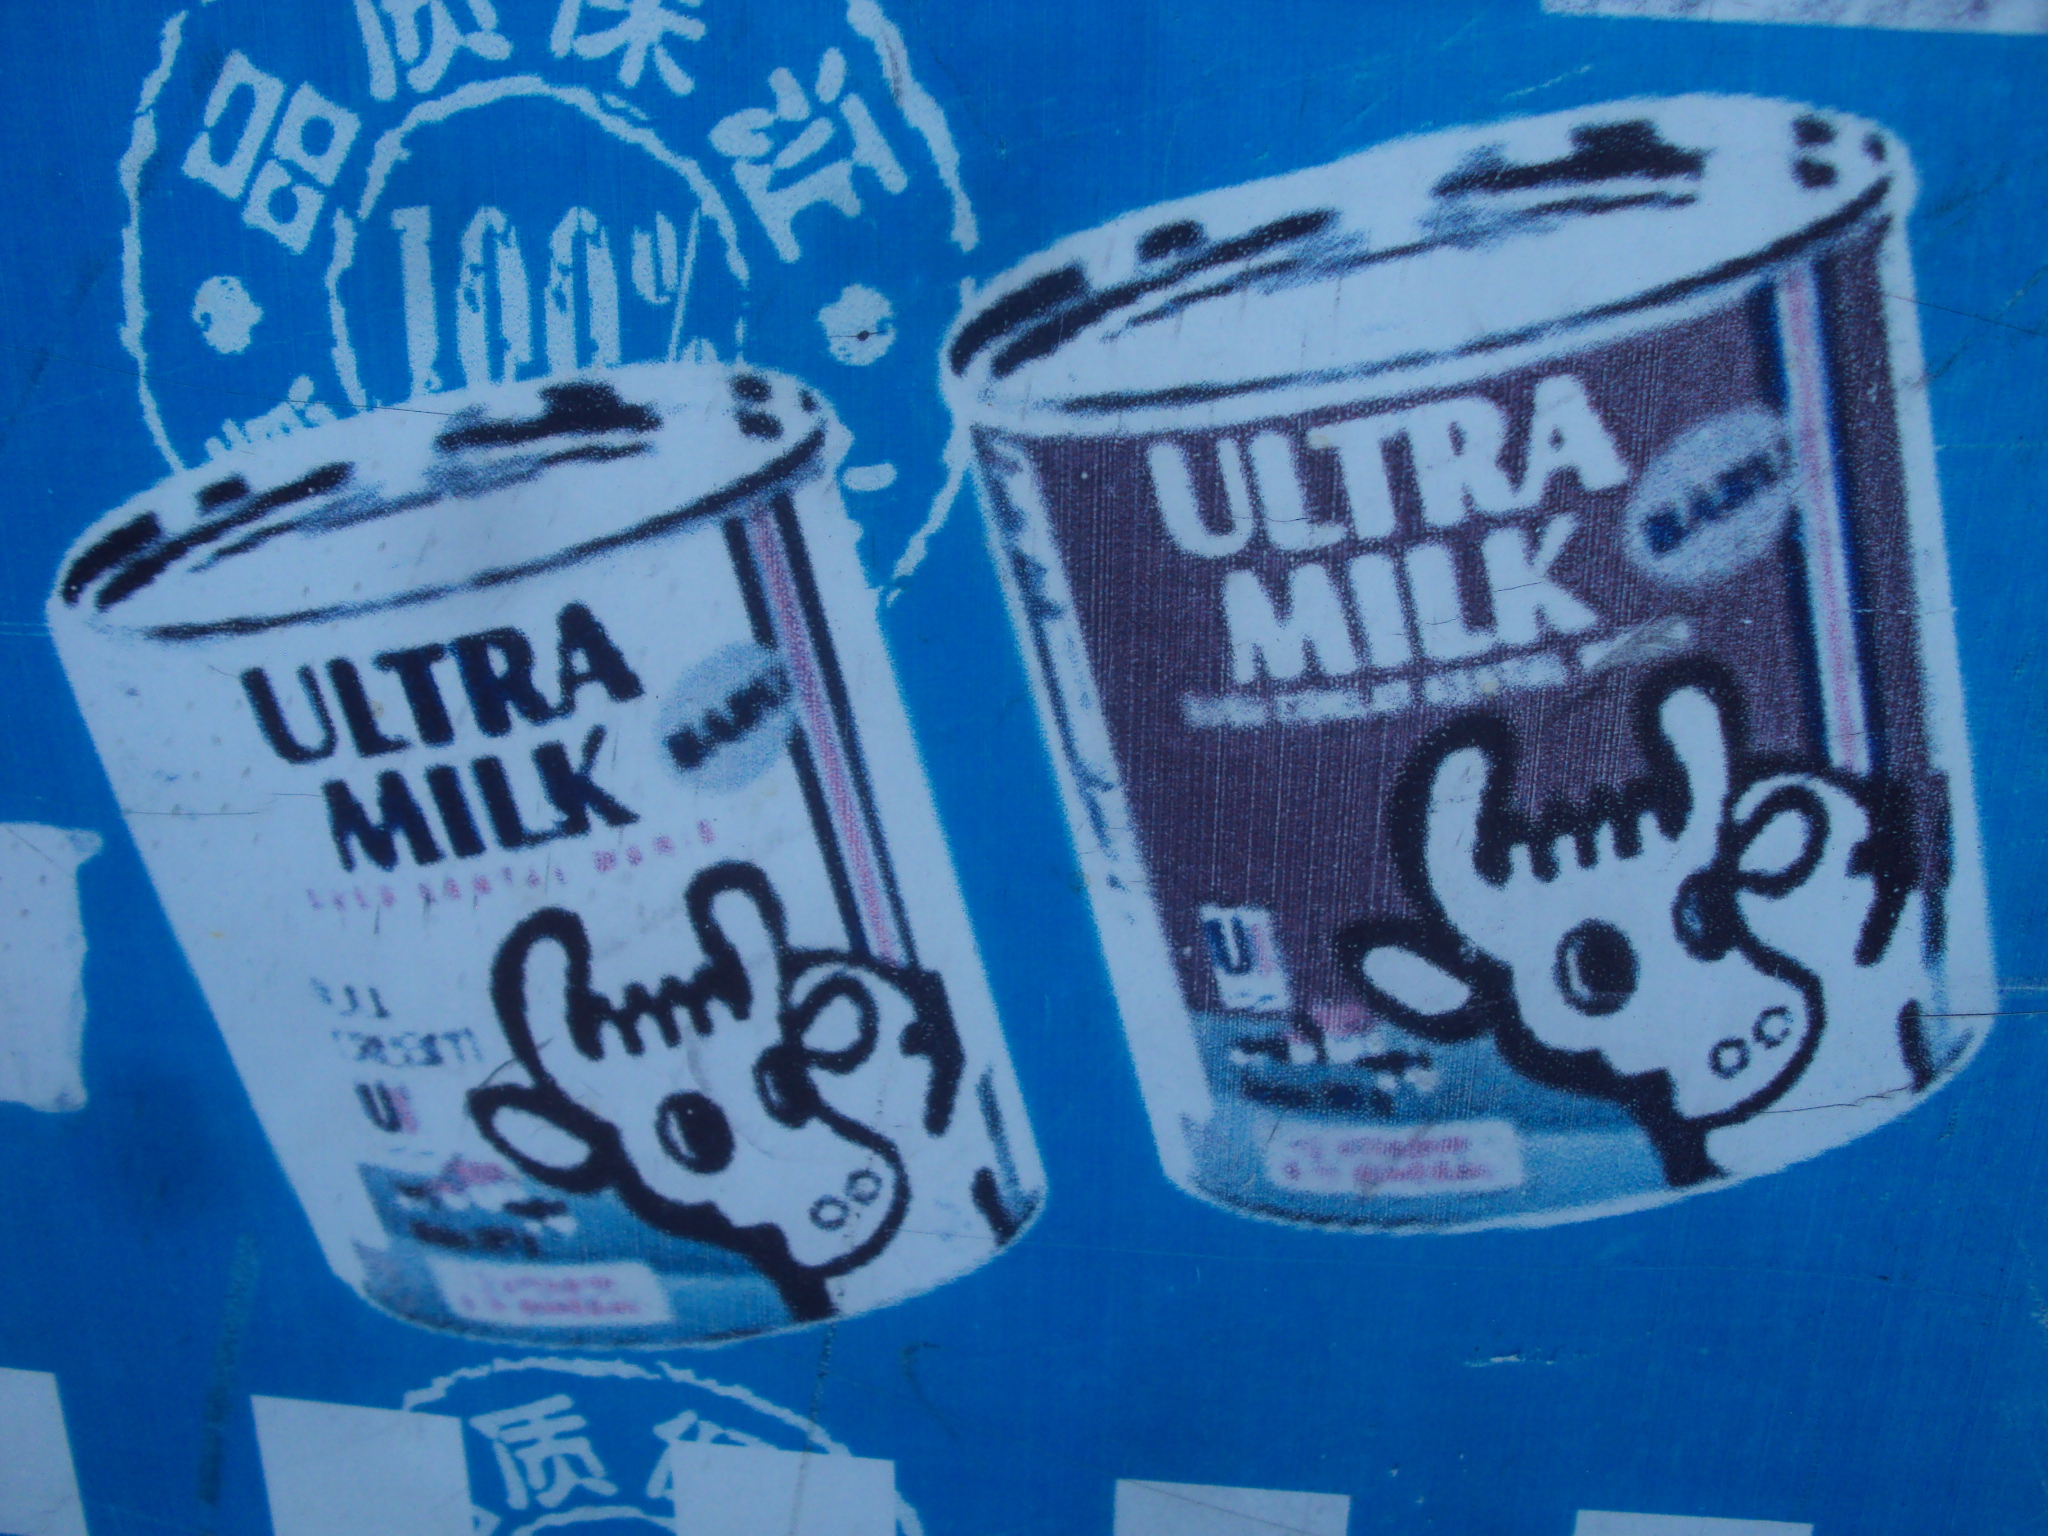
\includegraphics[width=5.19in]{landscape.jpg}

\vspace{0.25in}
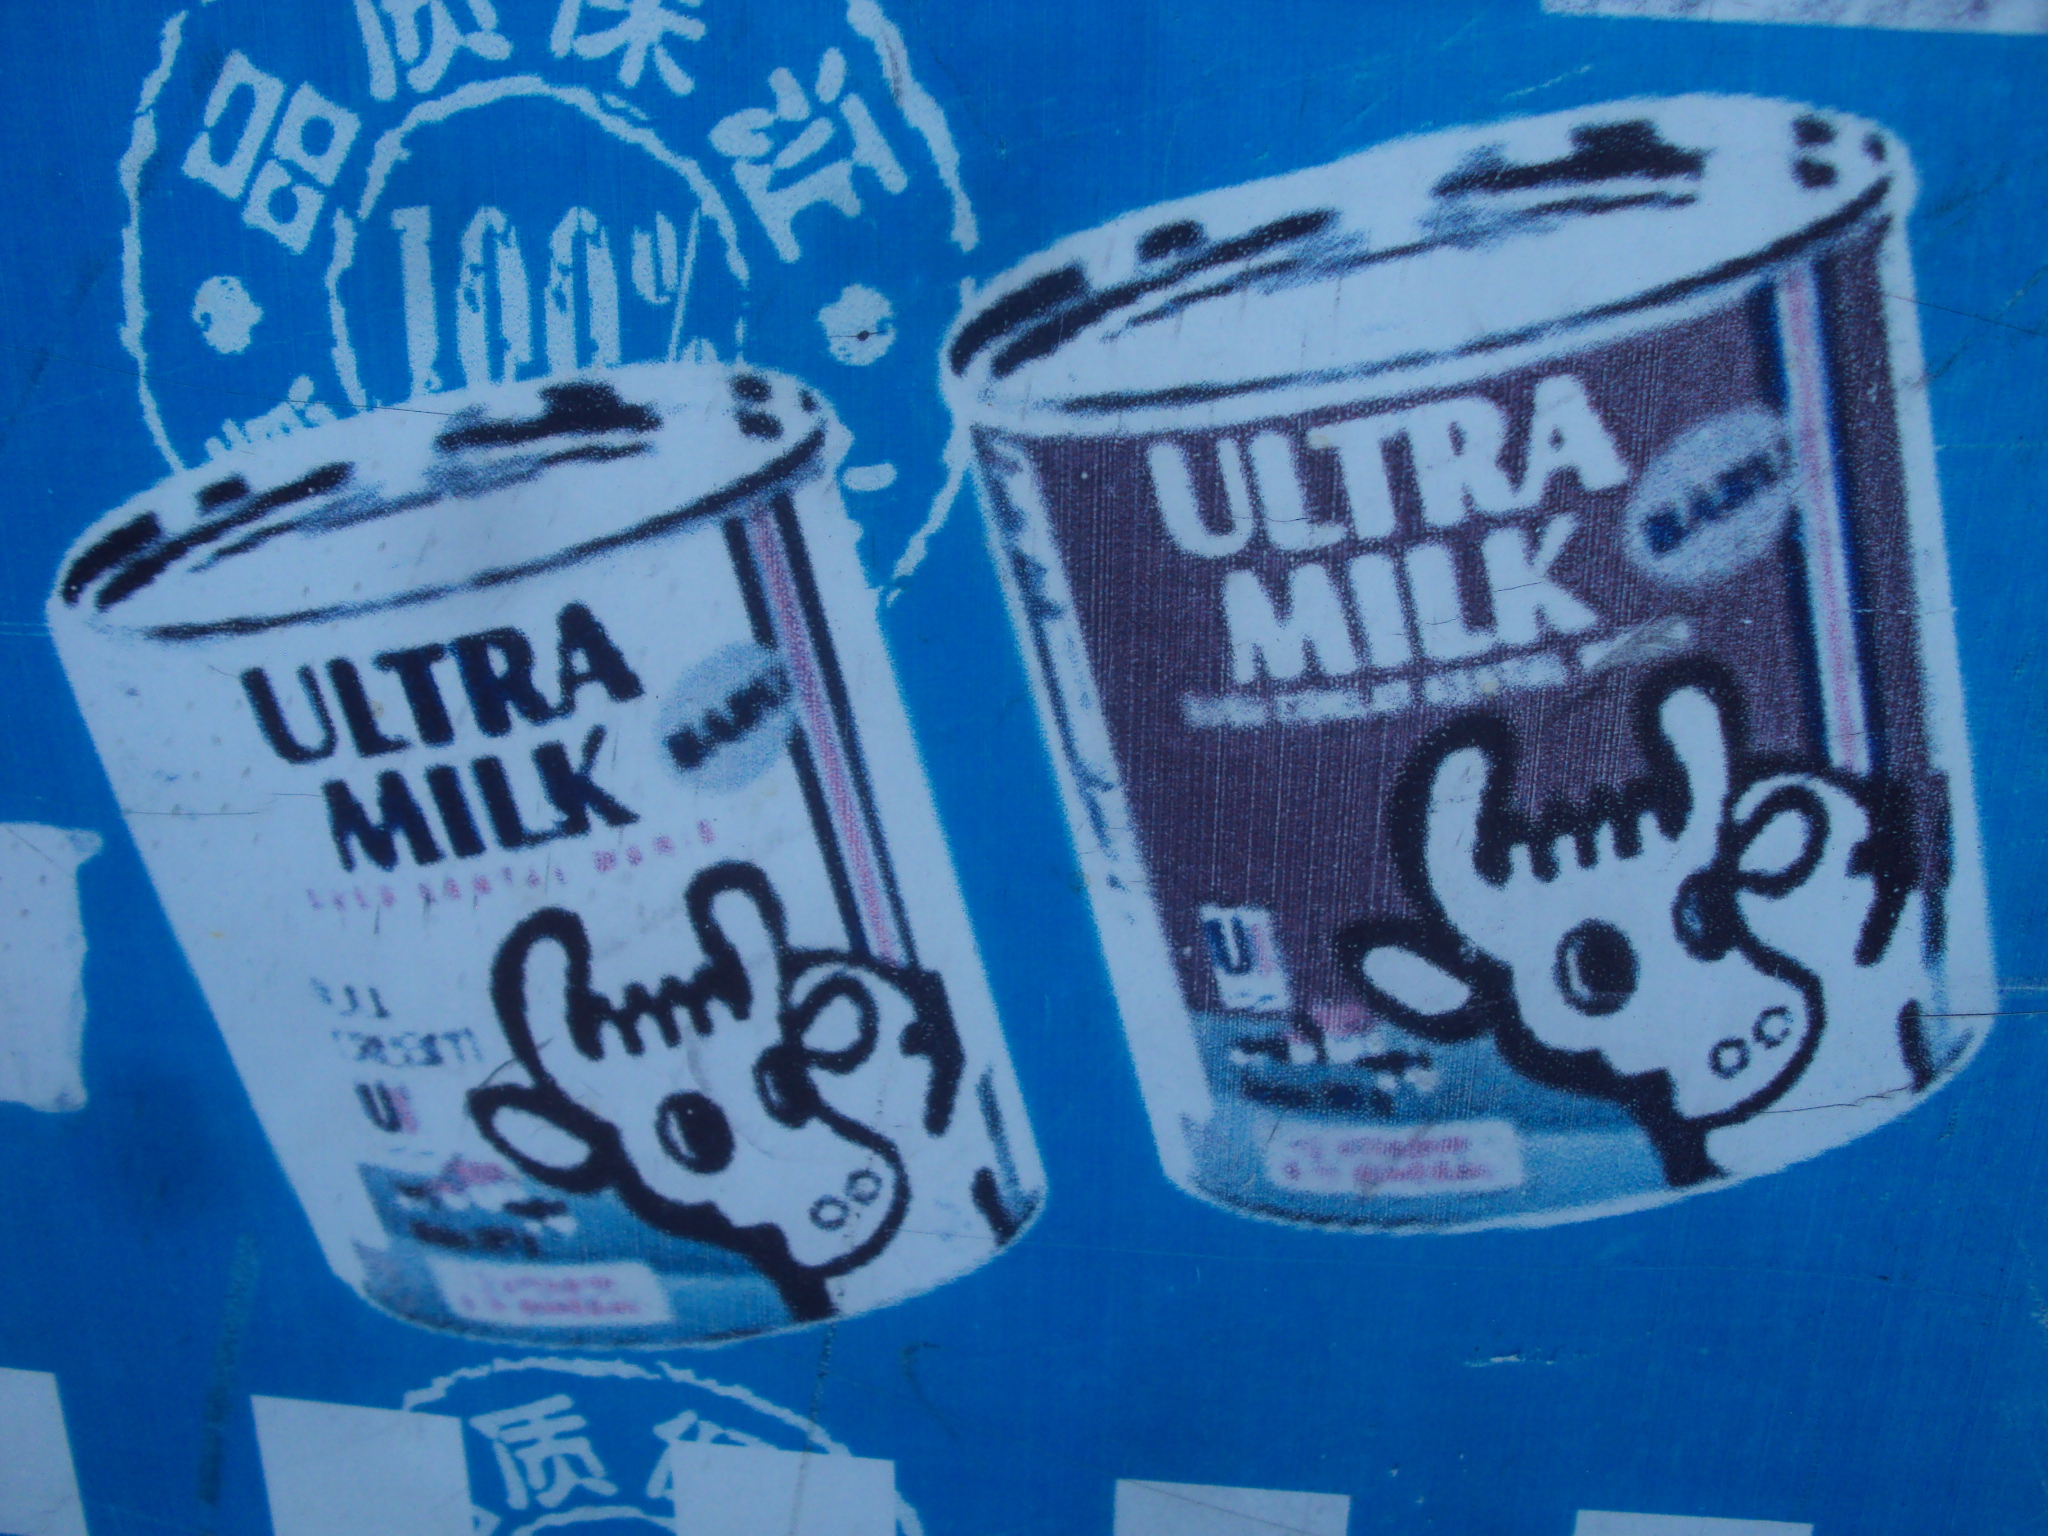
\includegraphics[width=5.19in]{landscape.jpg}

CAPTION L1\\
CAPTION L2\\
\pagebreak

% Layout L
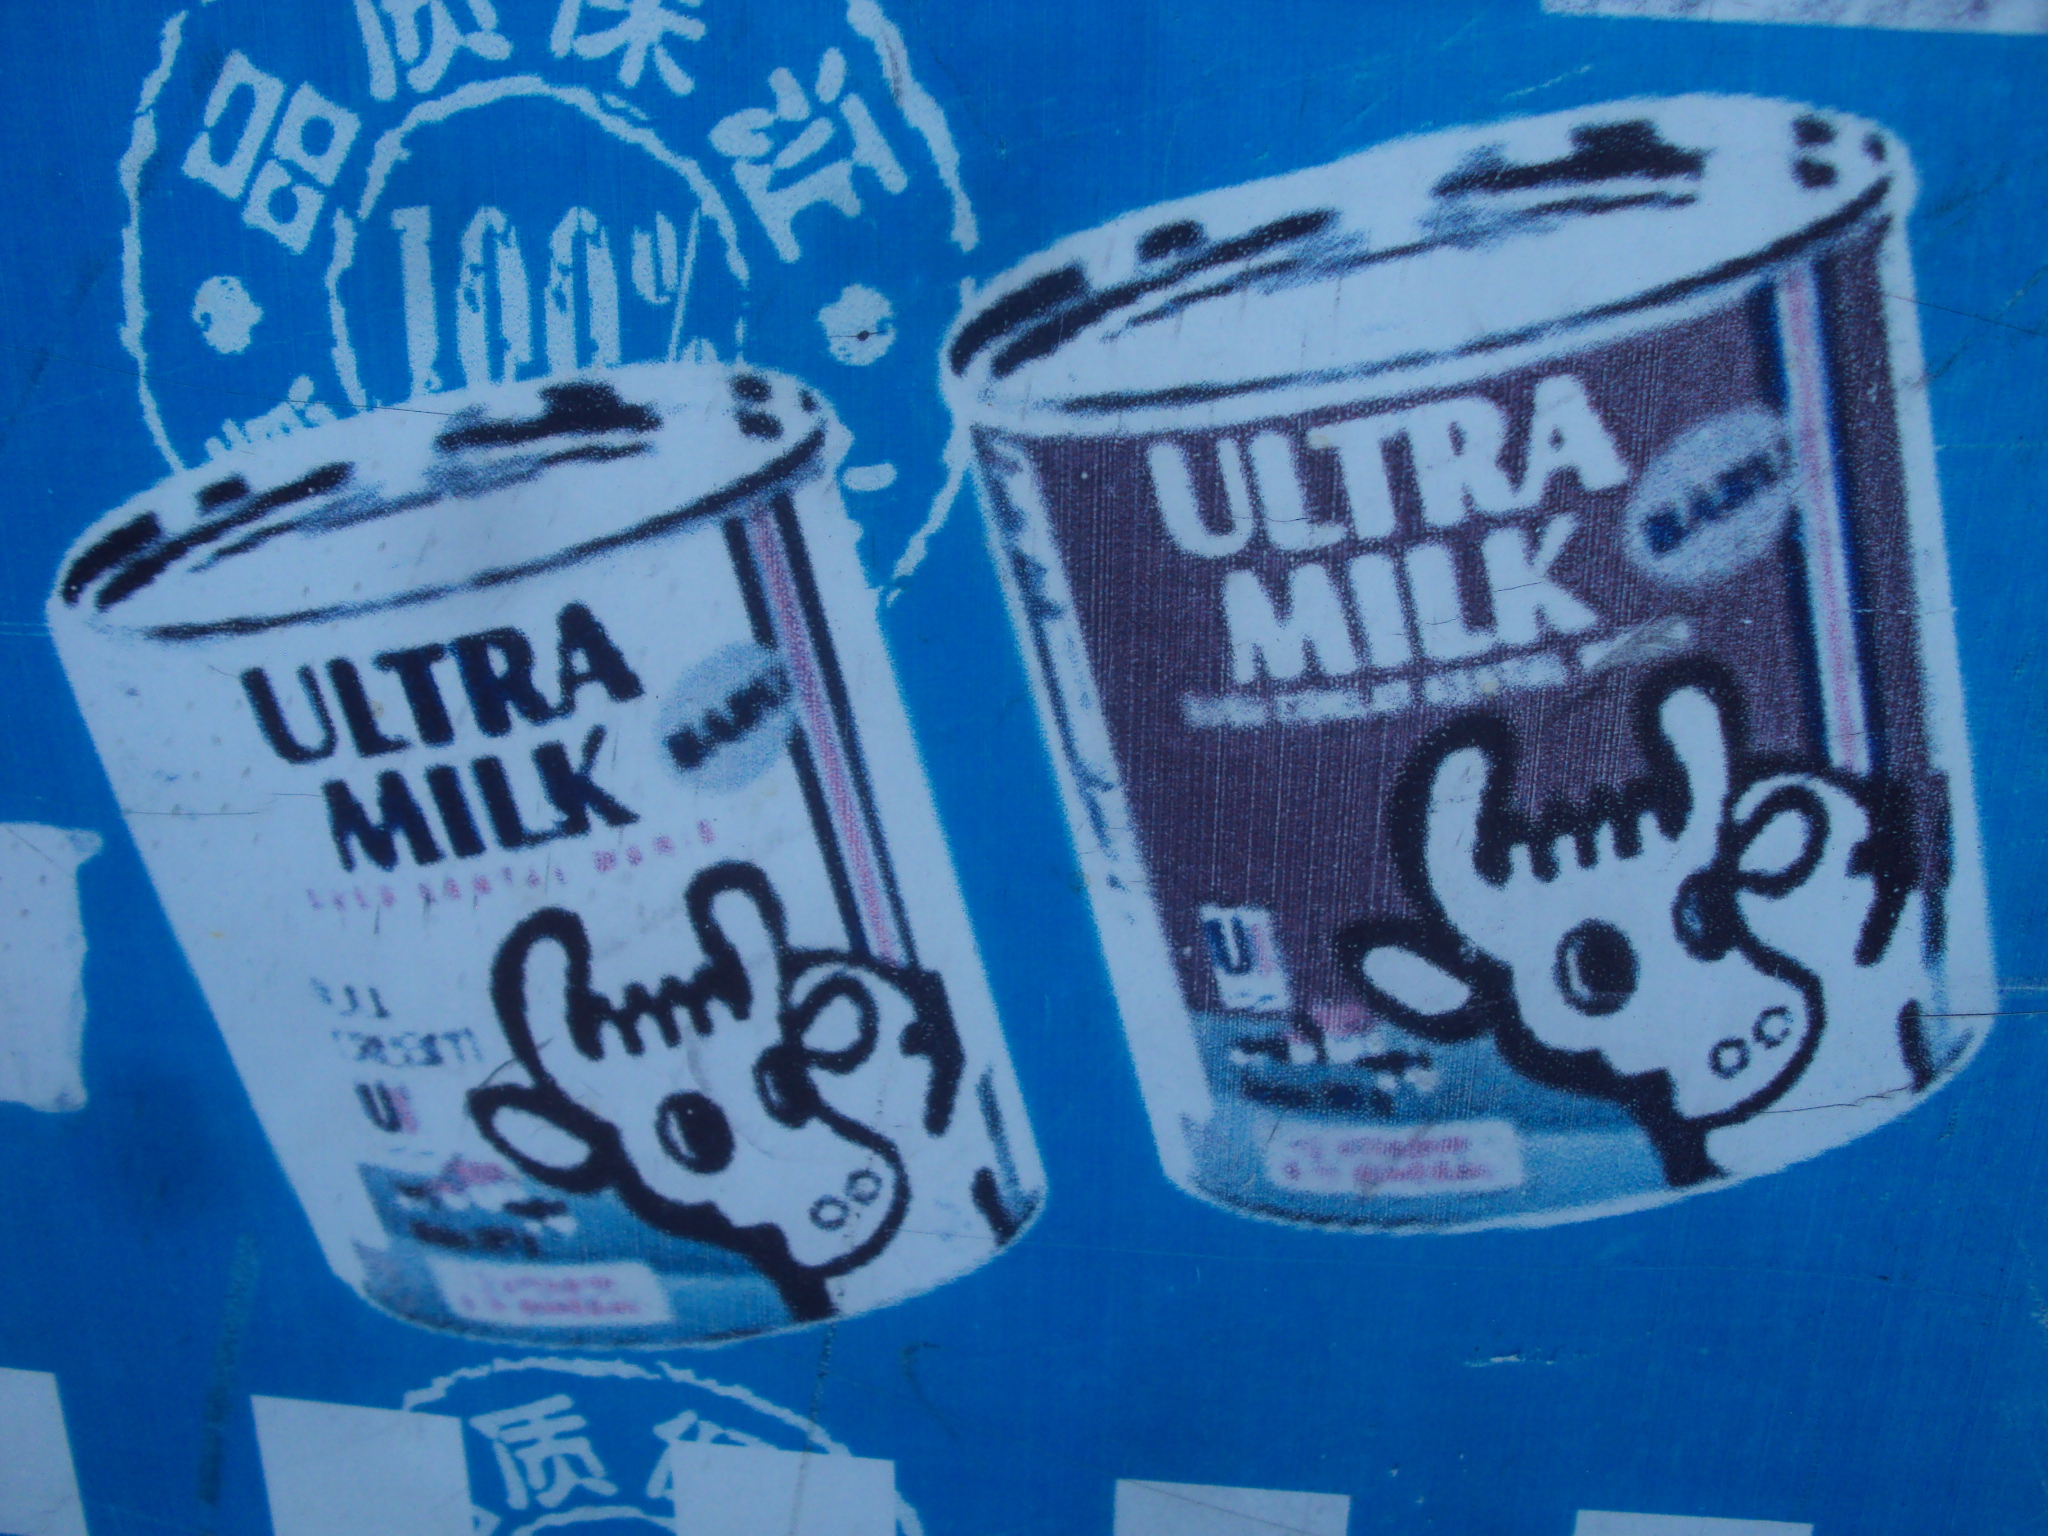
\includegraphics[width=5.19in]{landscape.jpg}

CAPTION L1\\
\pagebreak

% Layout PPPP
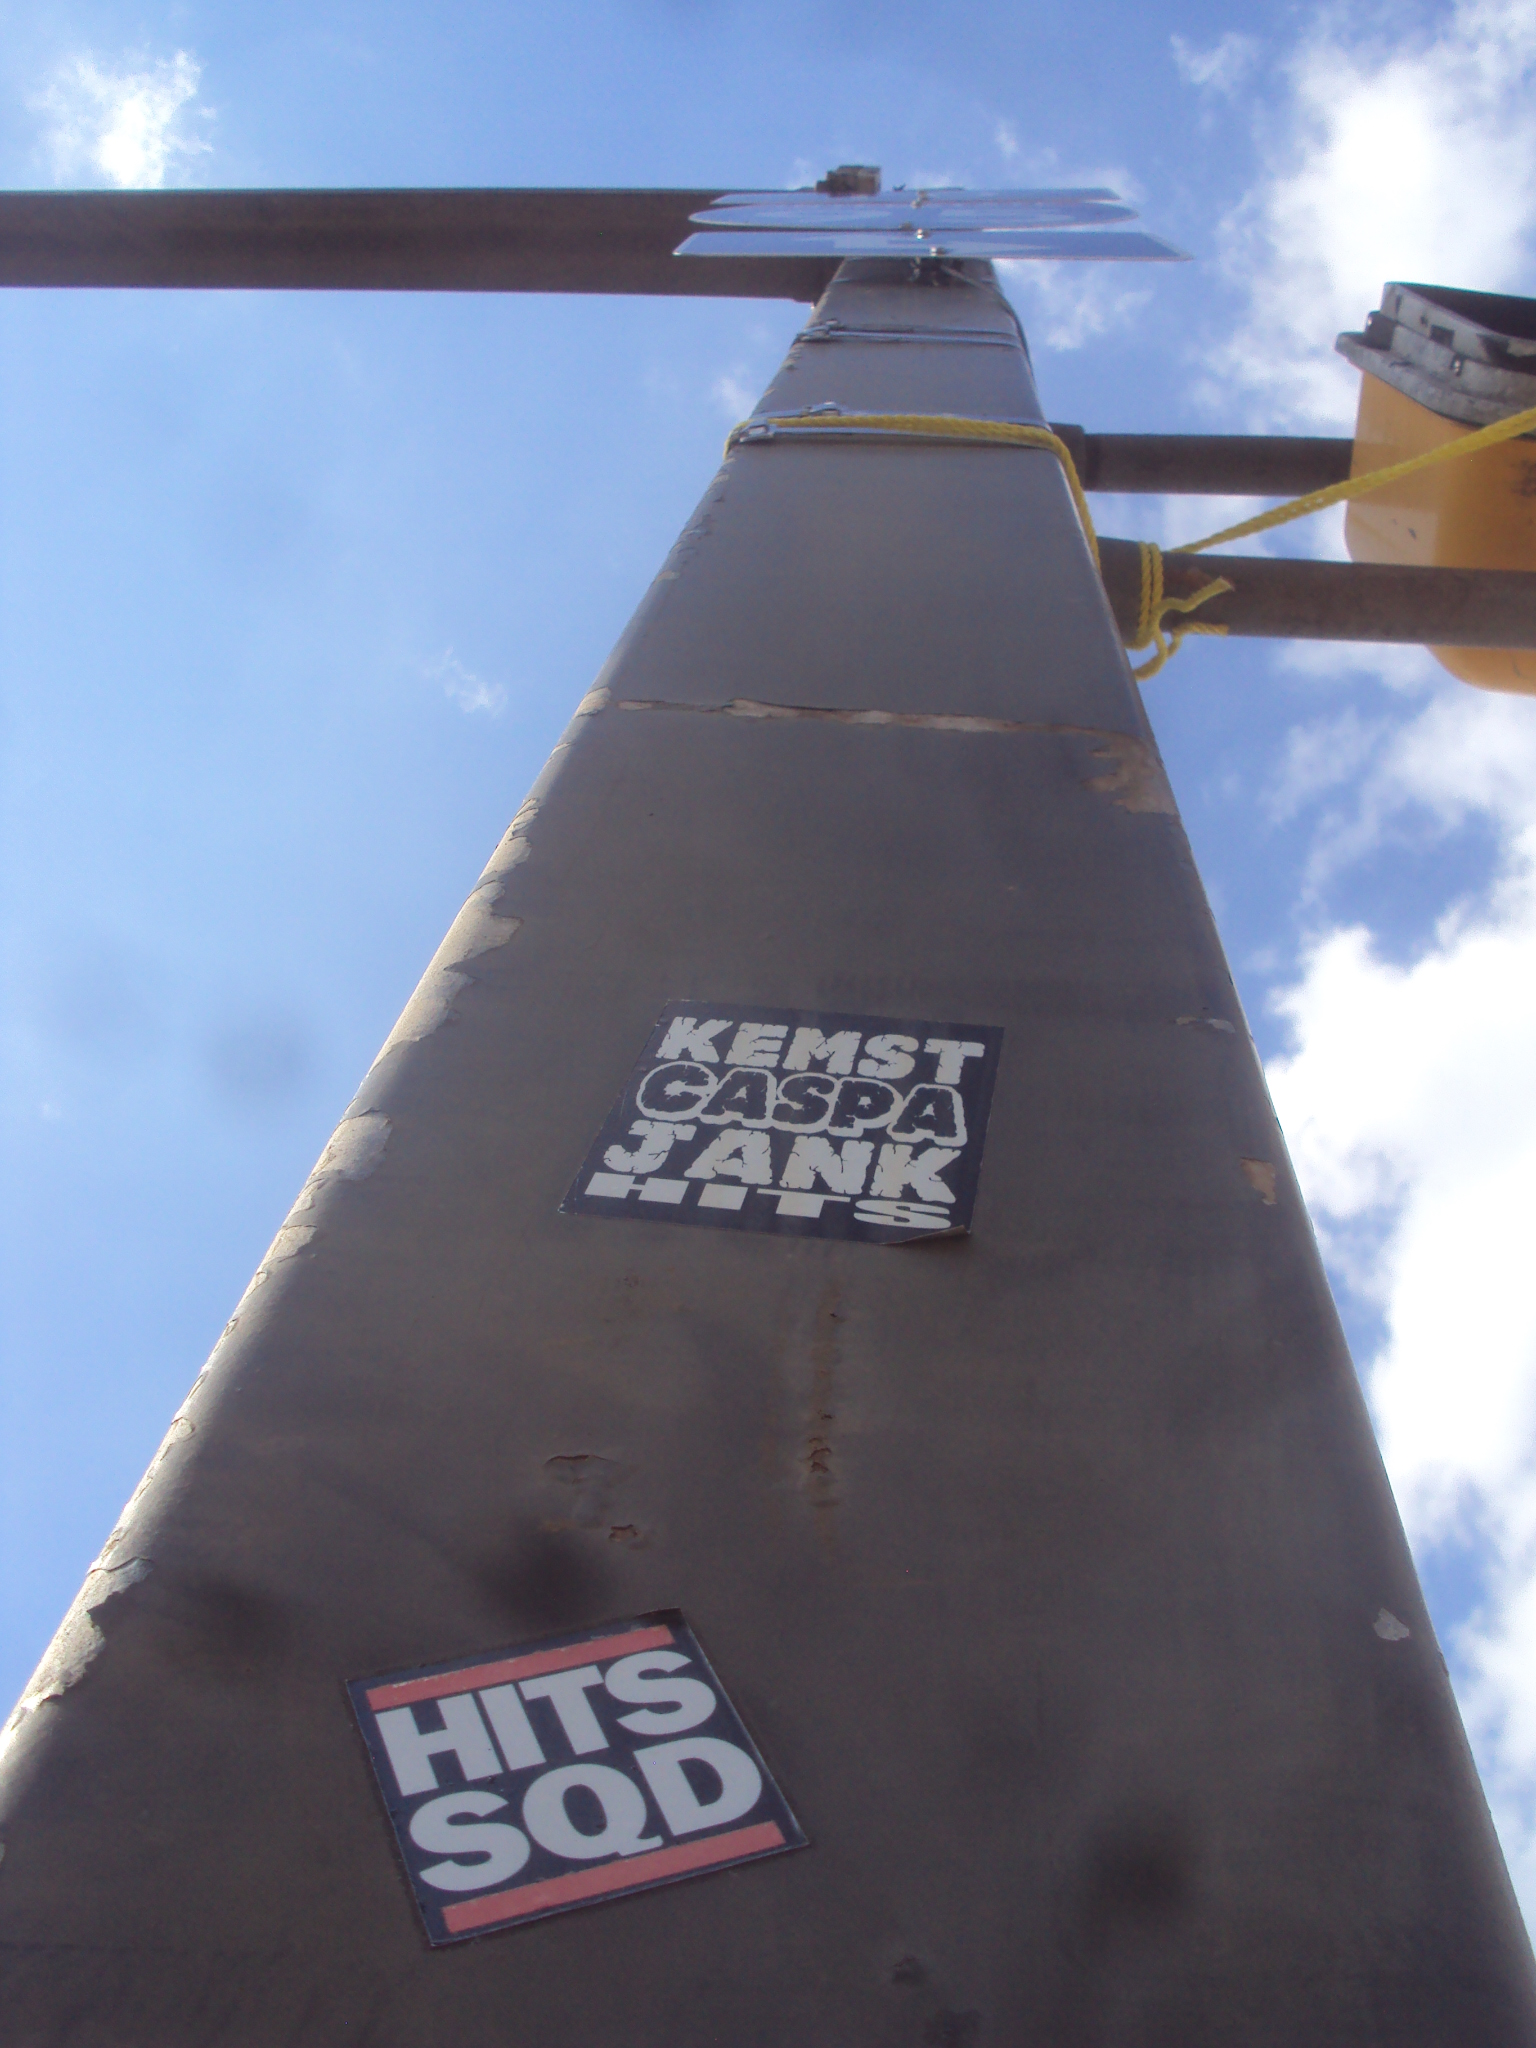
\includegraphics[height=4in]{portrait.jpg}
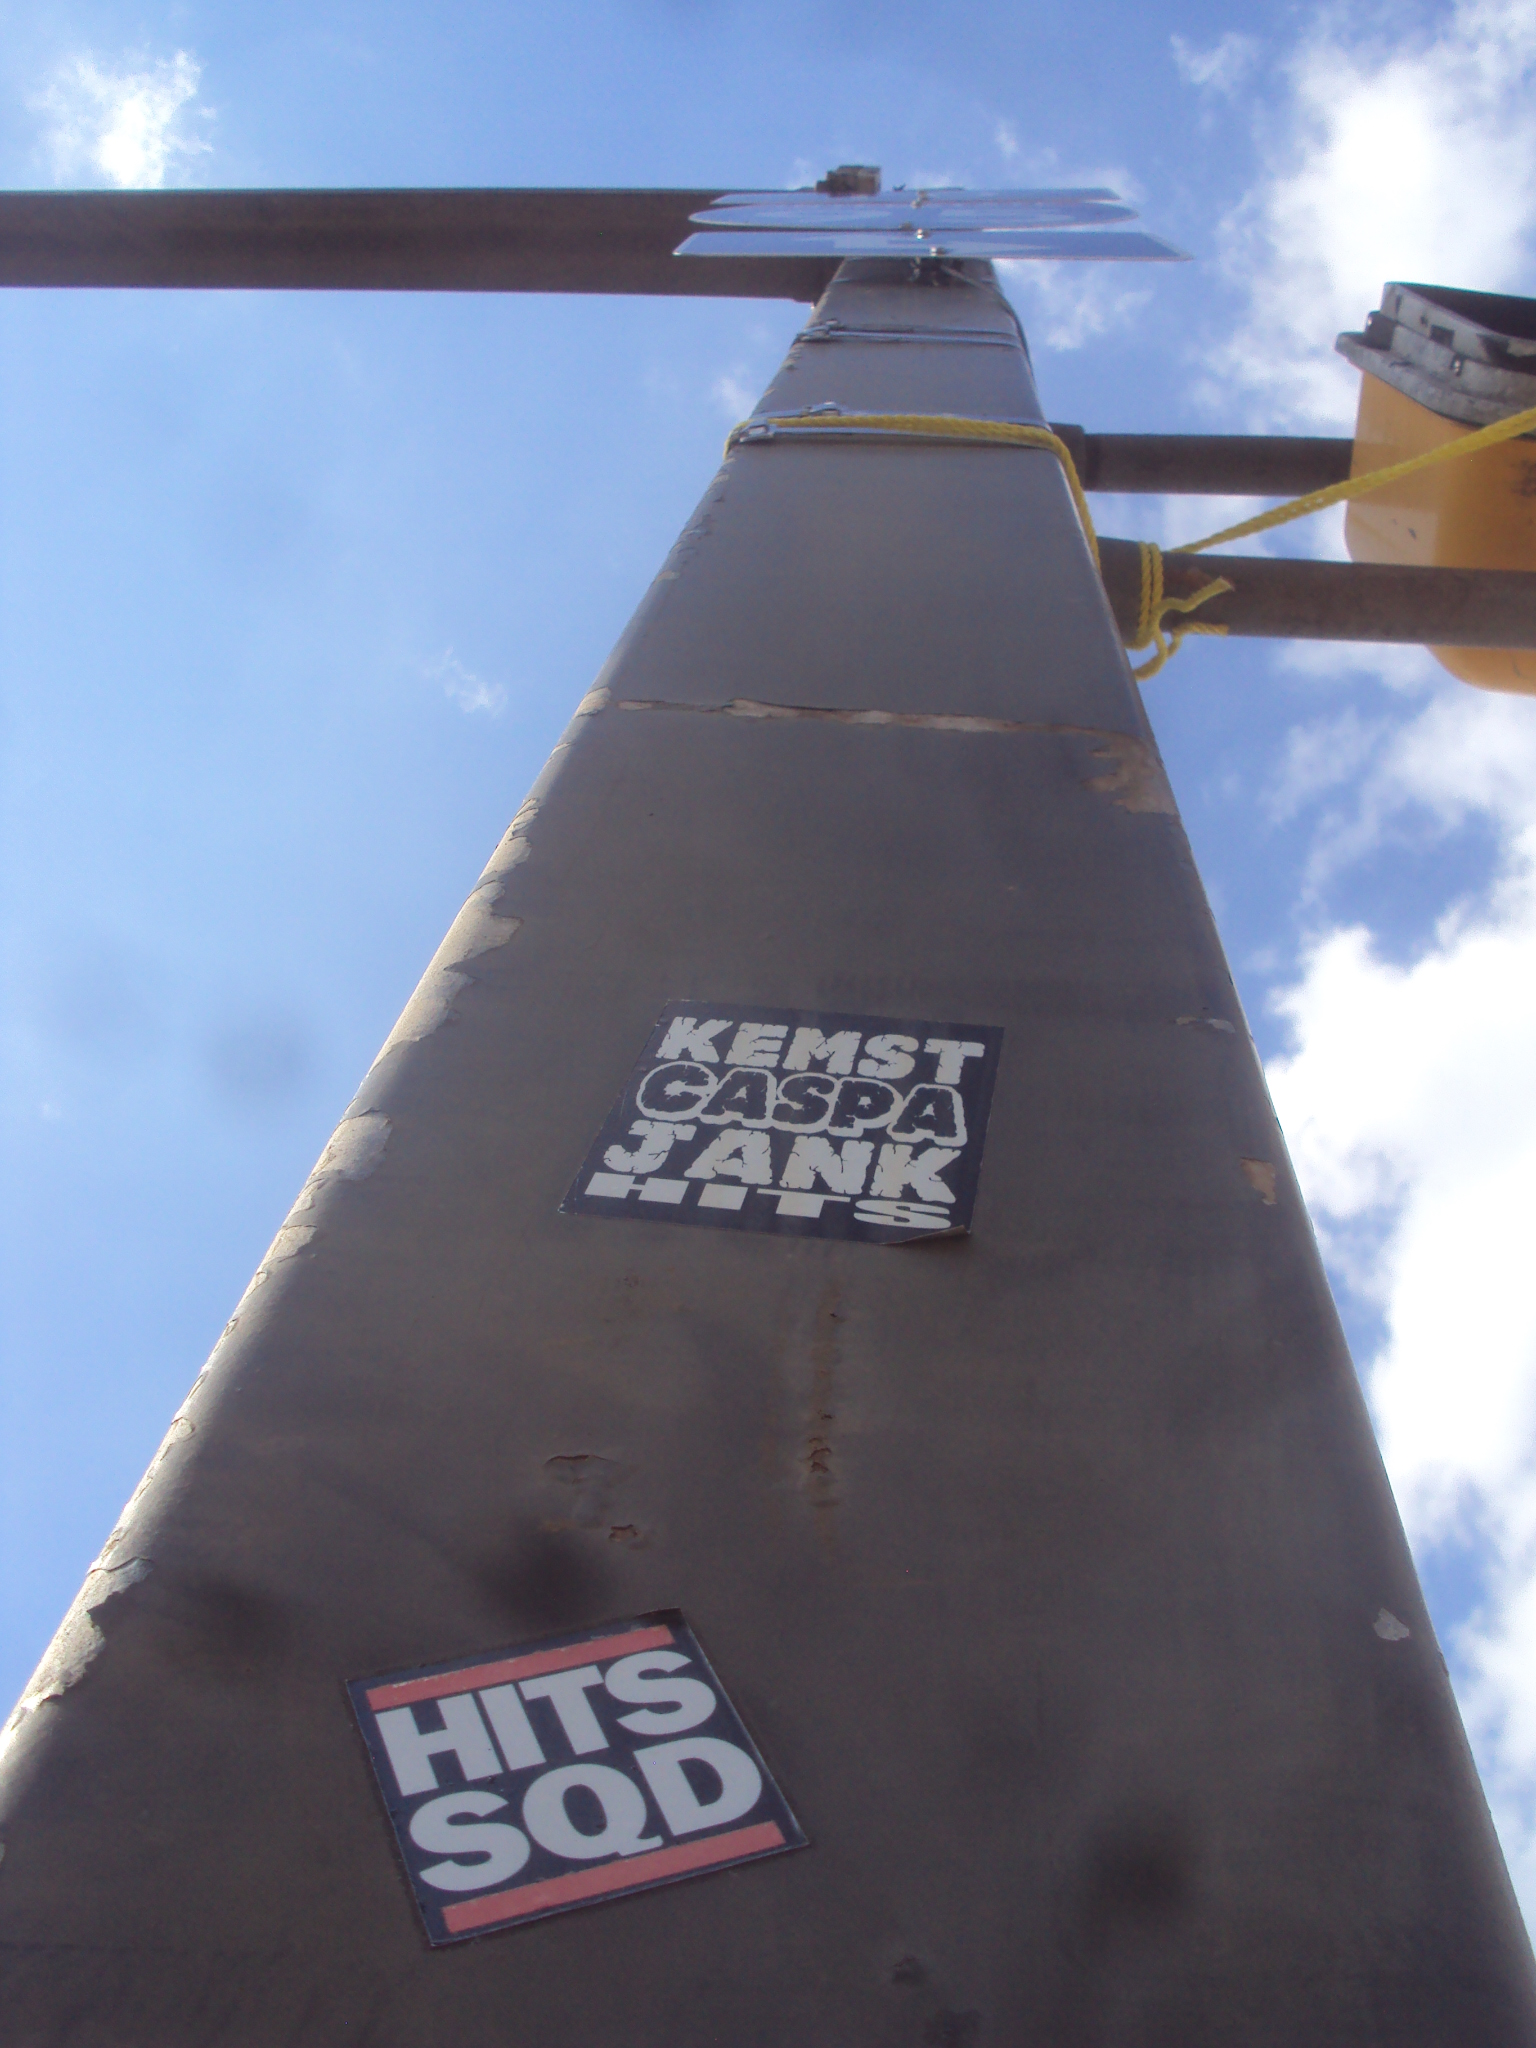
\includegraphics[height=4in]{portrait.jpg}

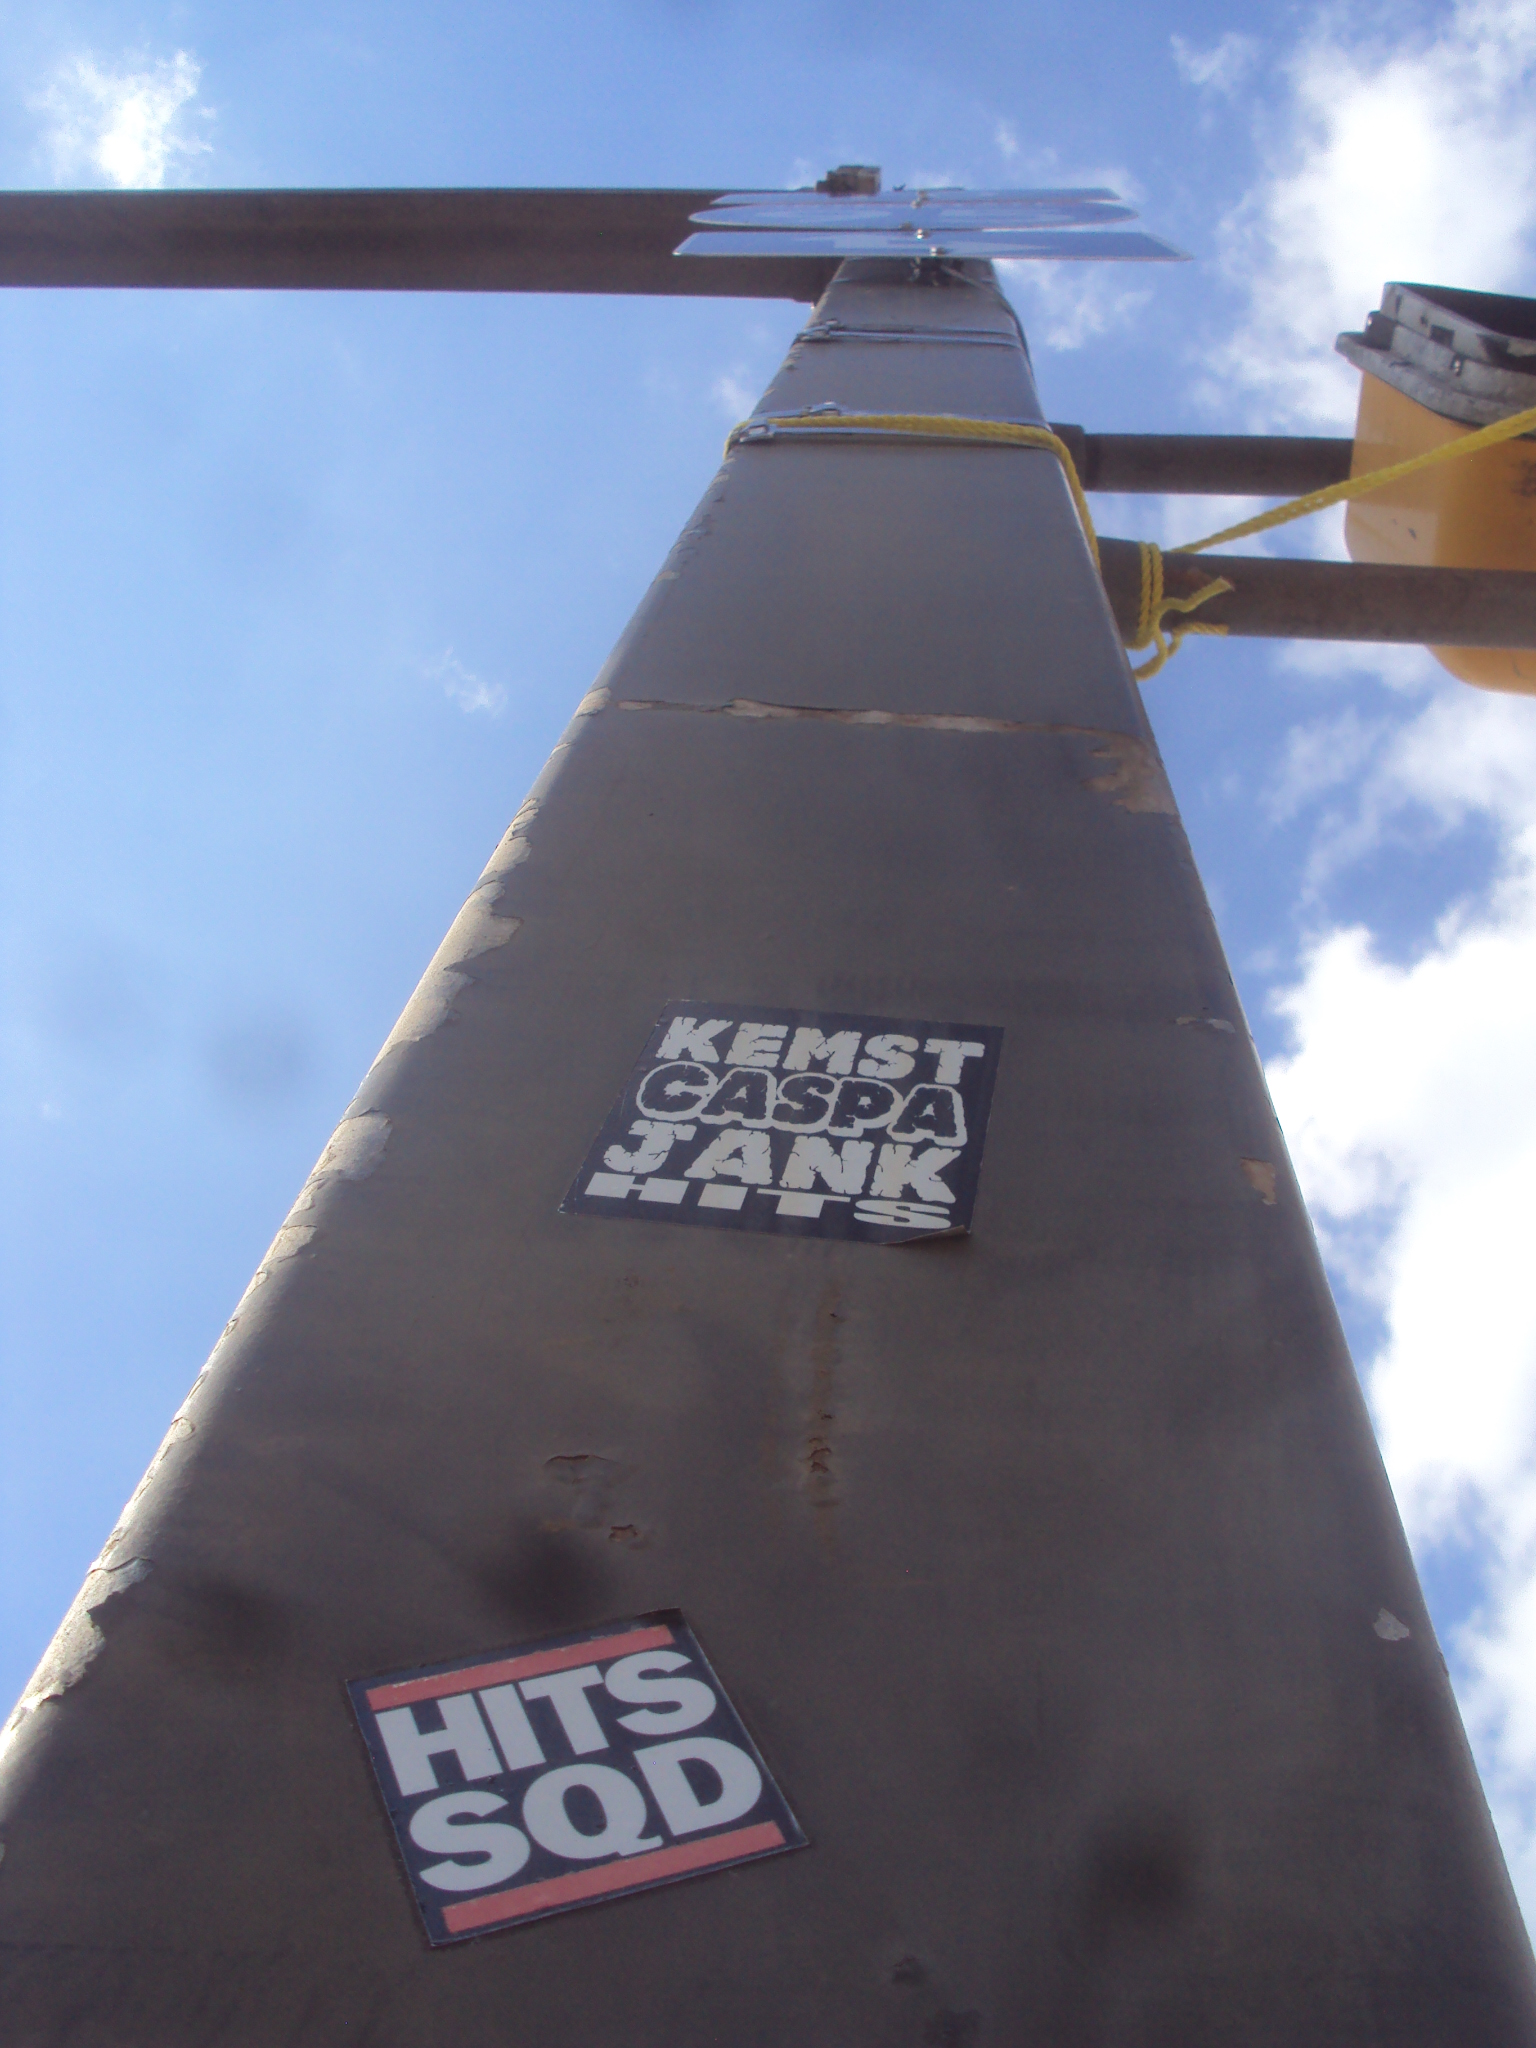
\includegraphics[height=4in]{portrait.jpg}
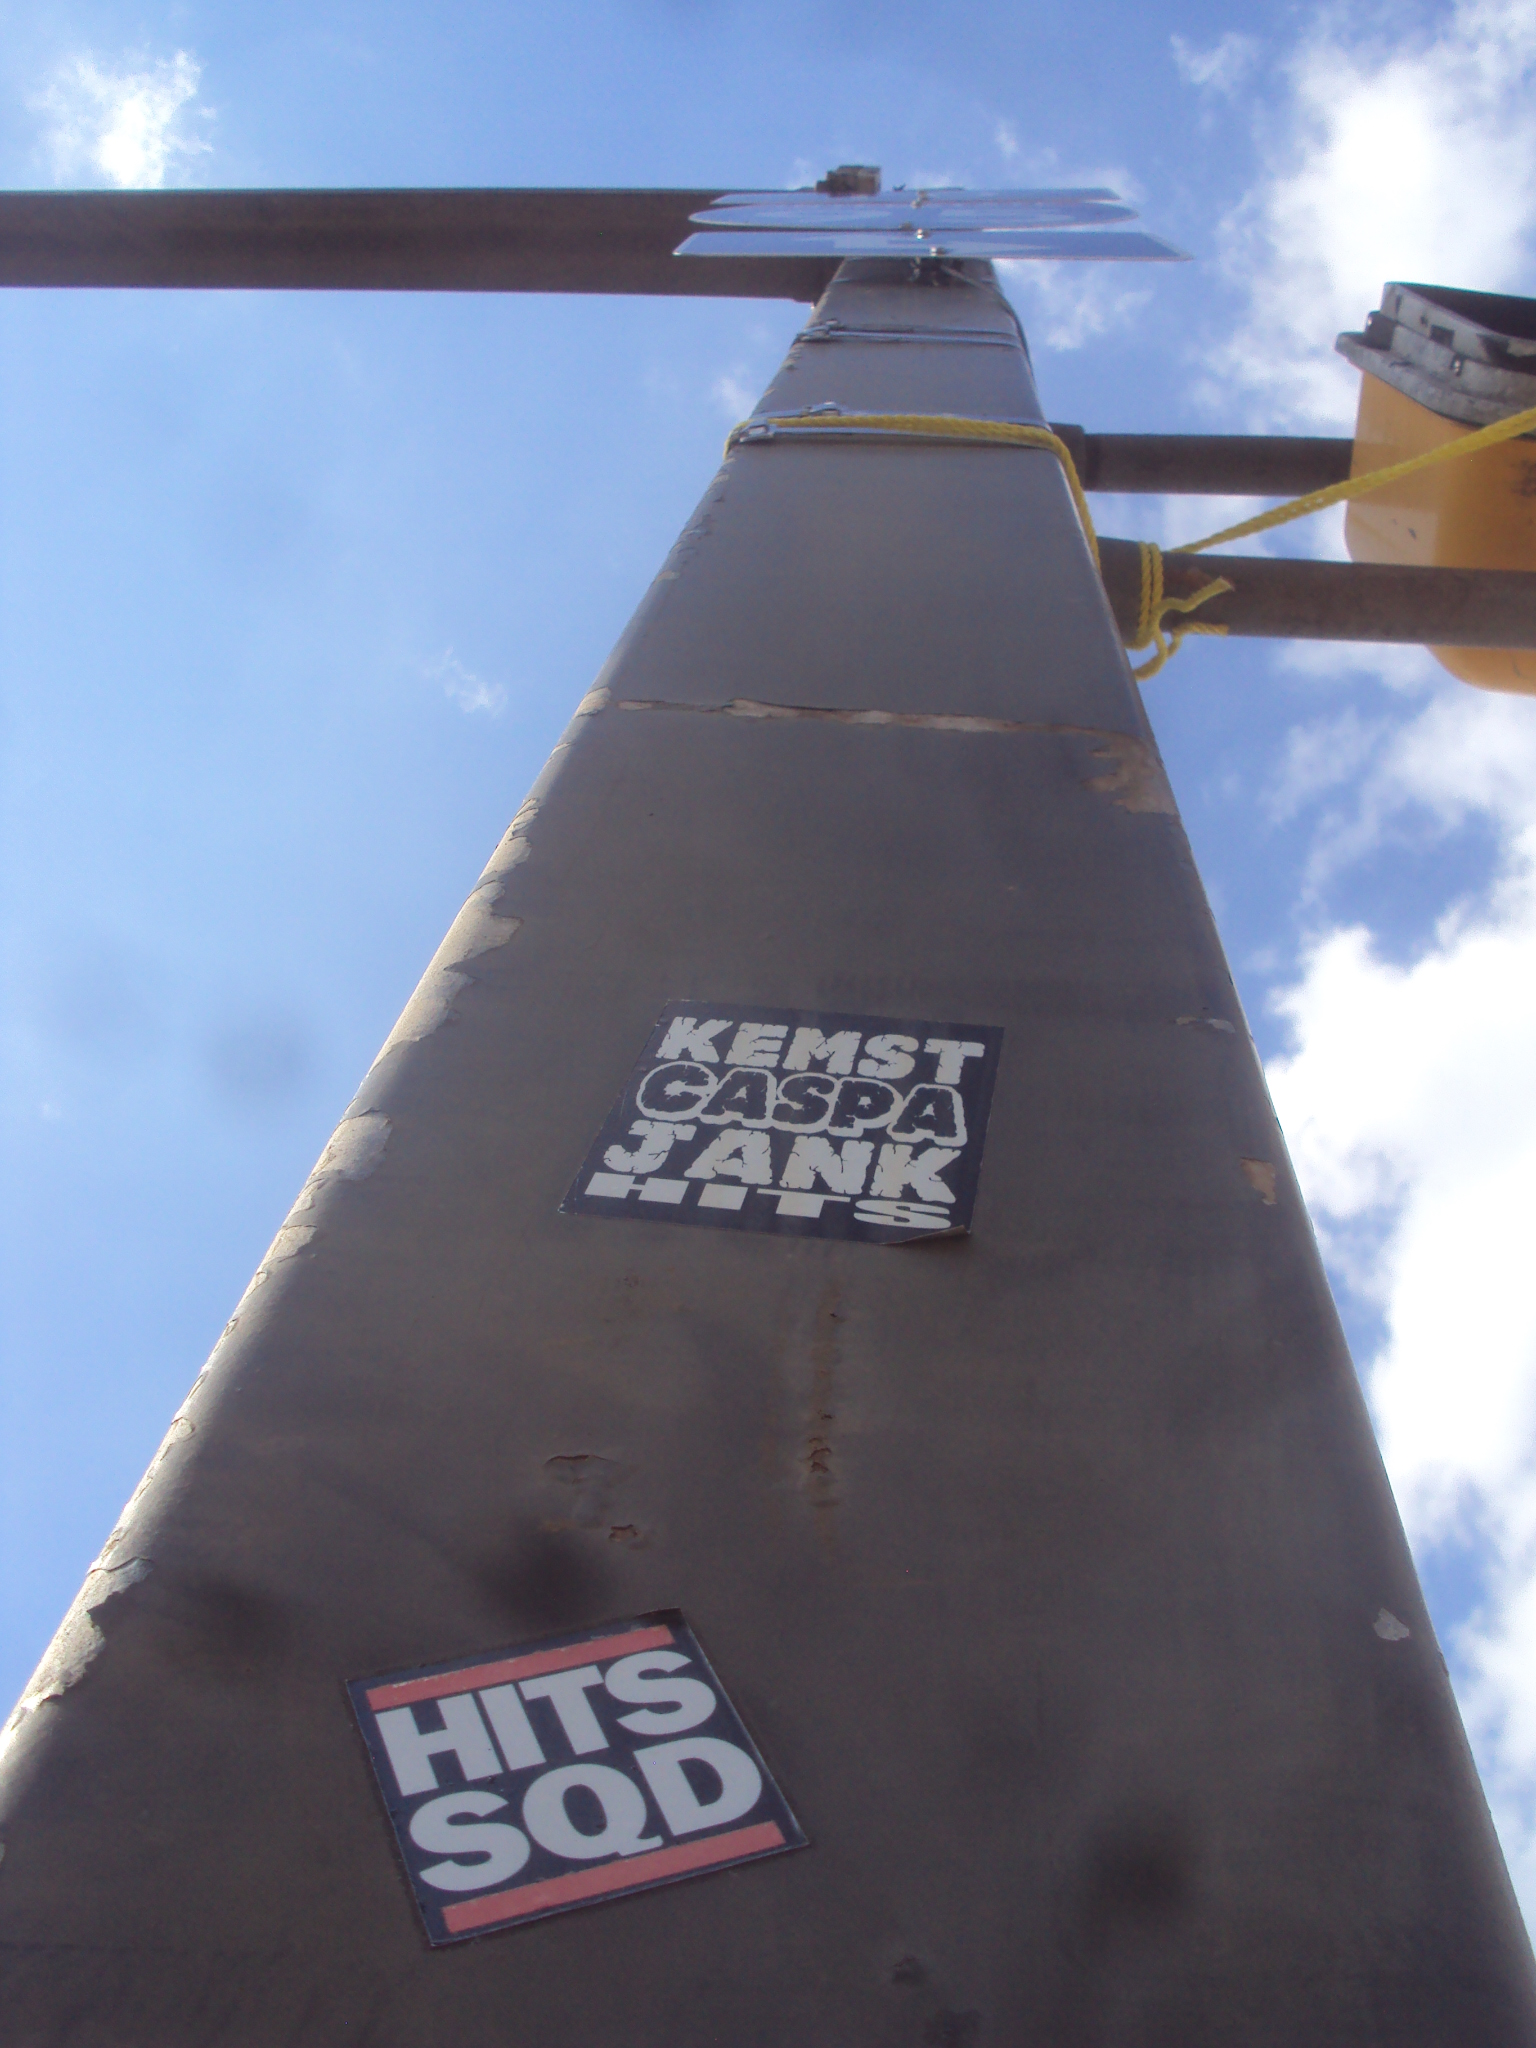
\includegraphics[height=4in]{portrait.jpg}

CAPTION P1\\
CAPTION P2\\
CAPTION P3\\
CAPTION P4\\
\pagebreak

% Layout PPP
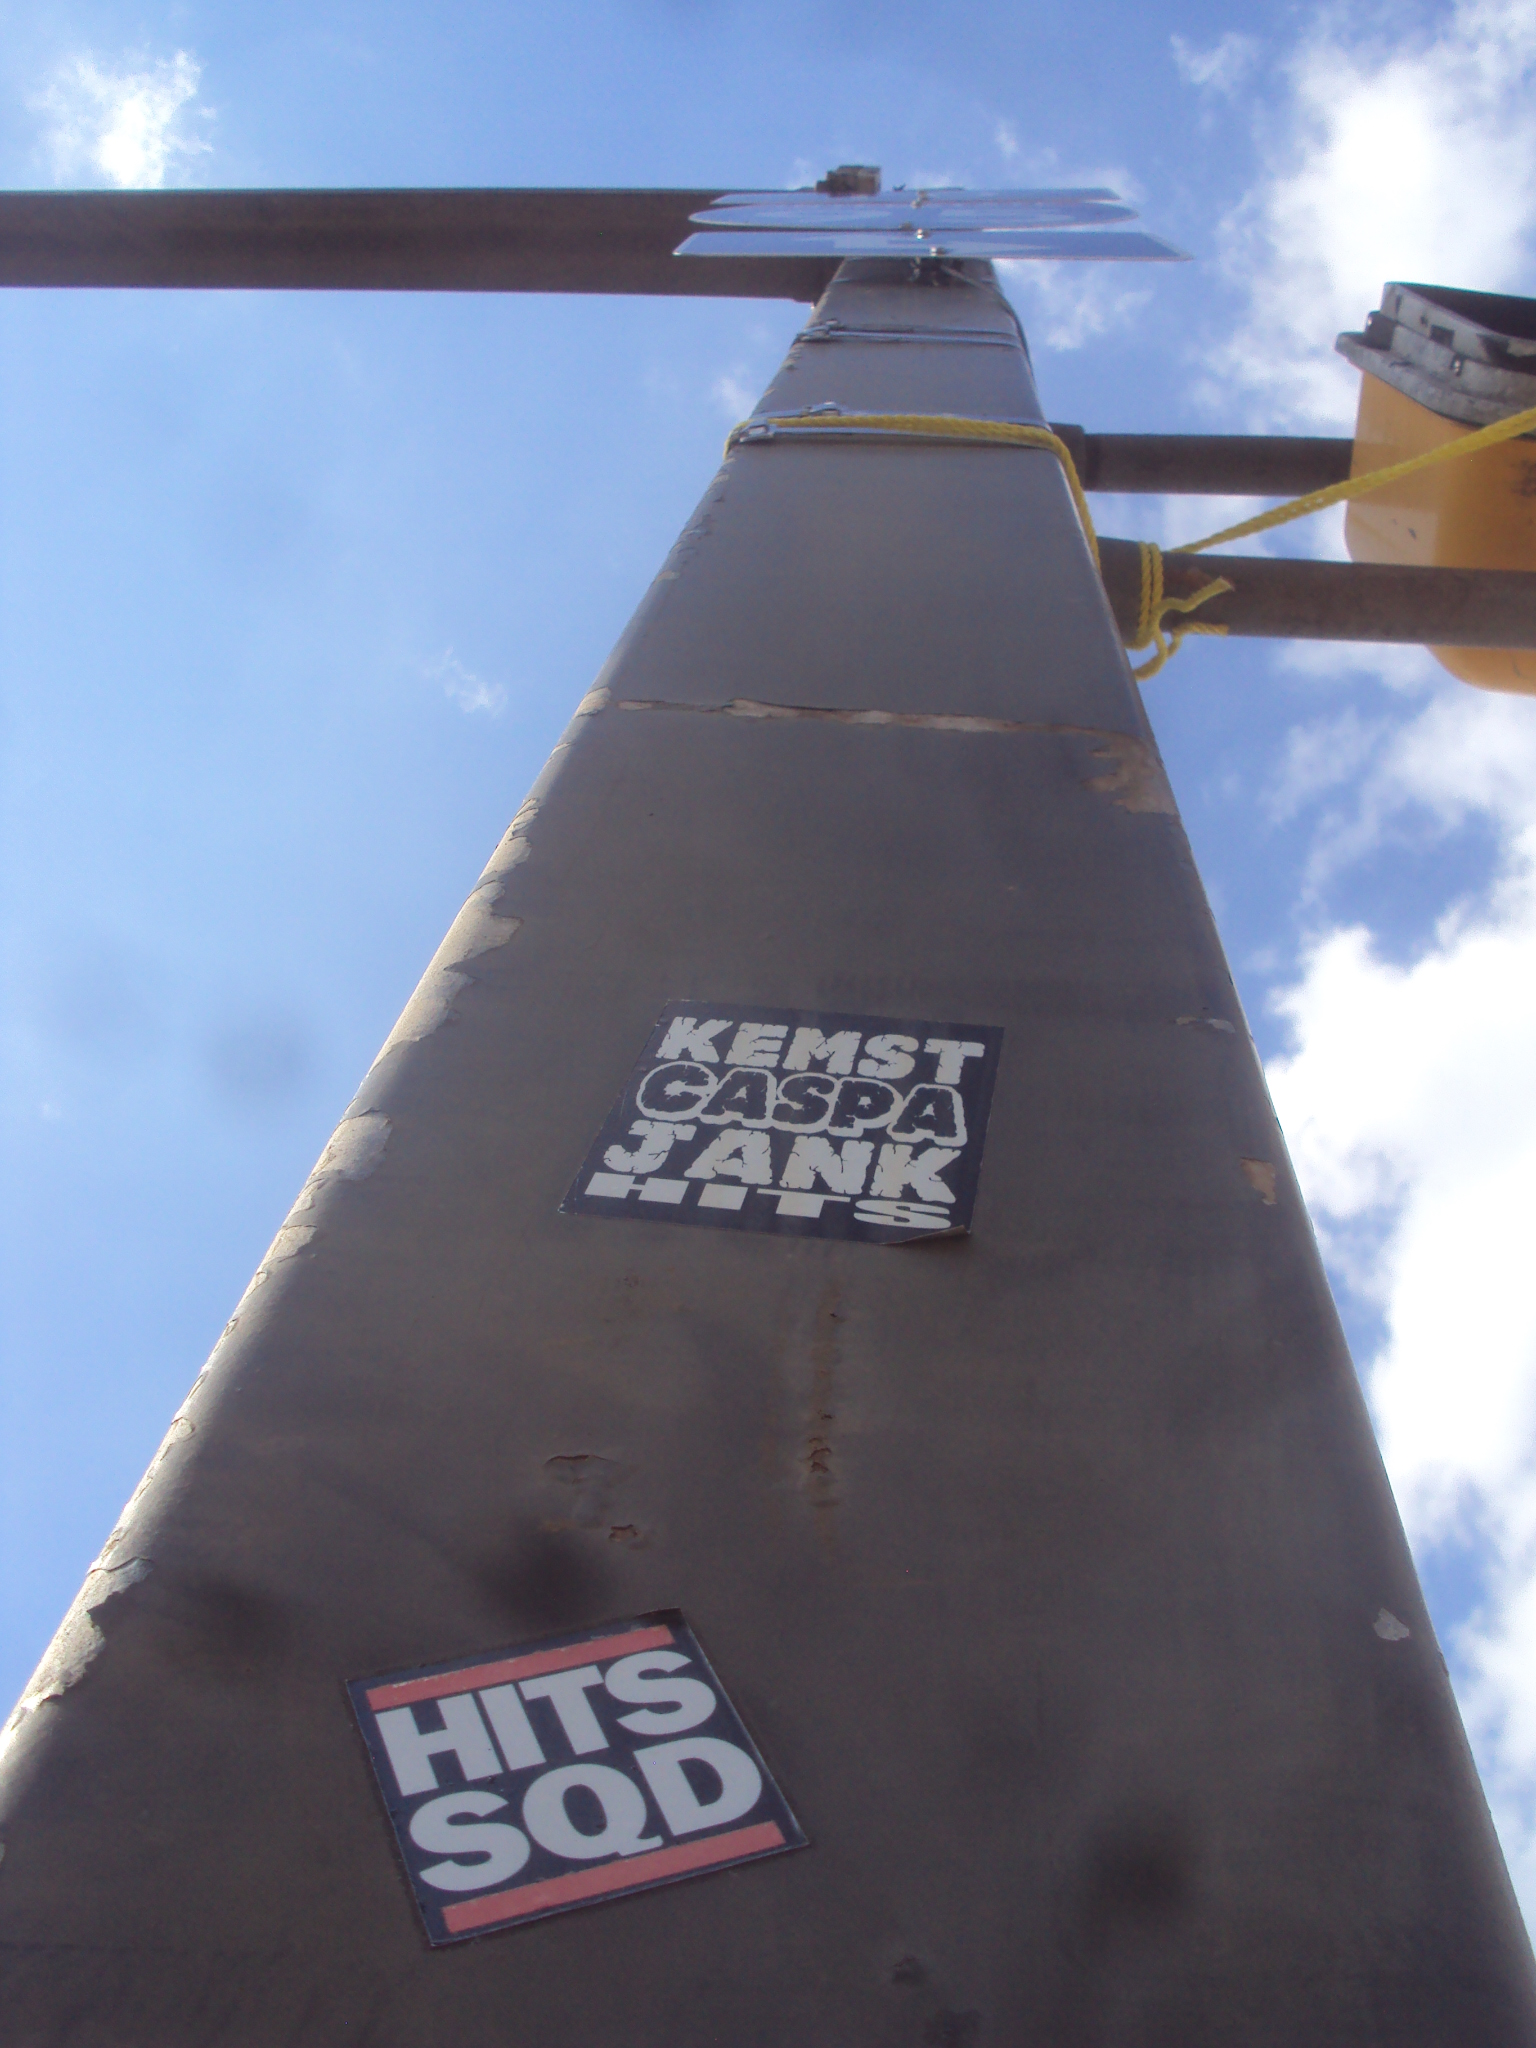
\includegraphics[height=4in]{portrait.jpg}
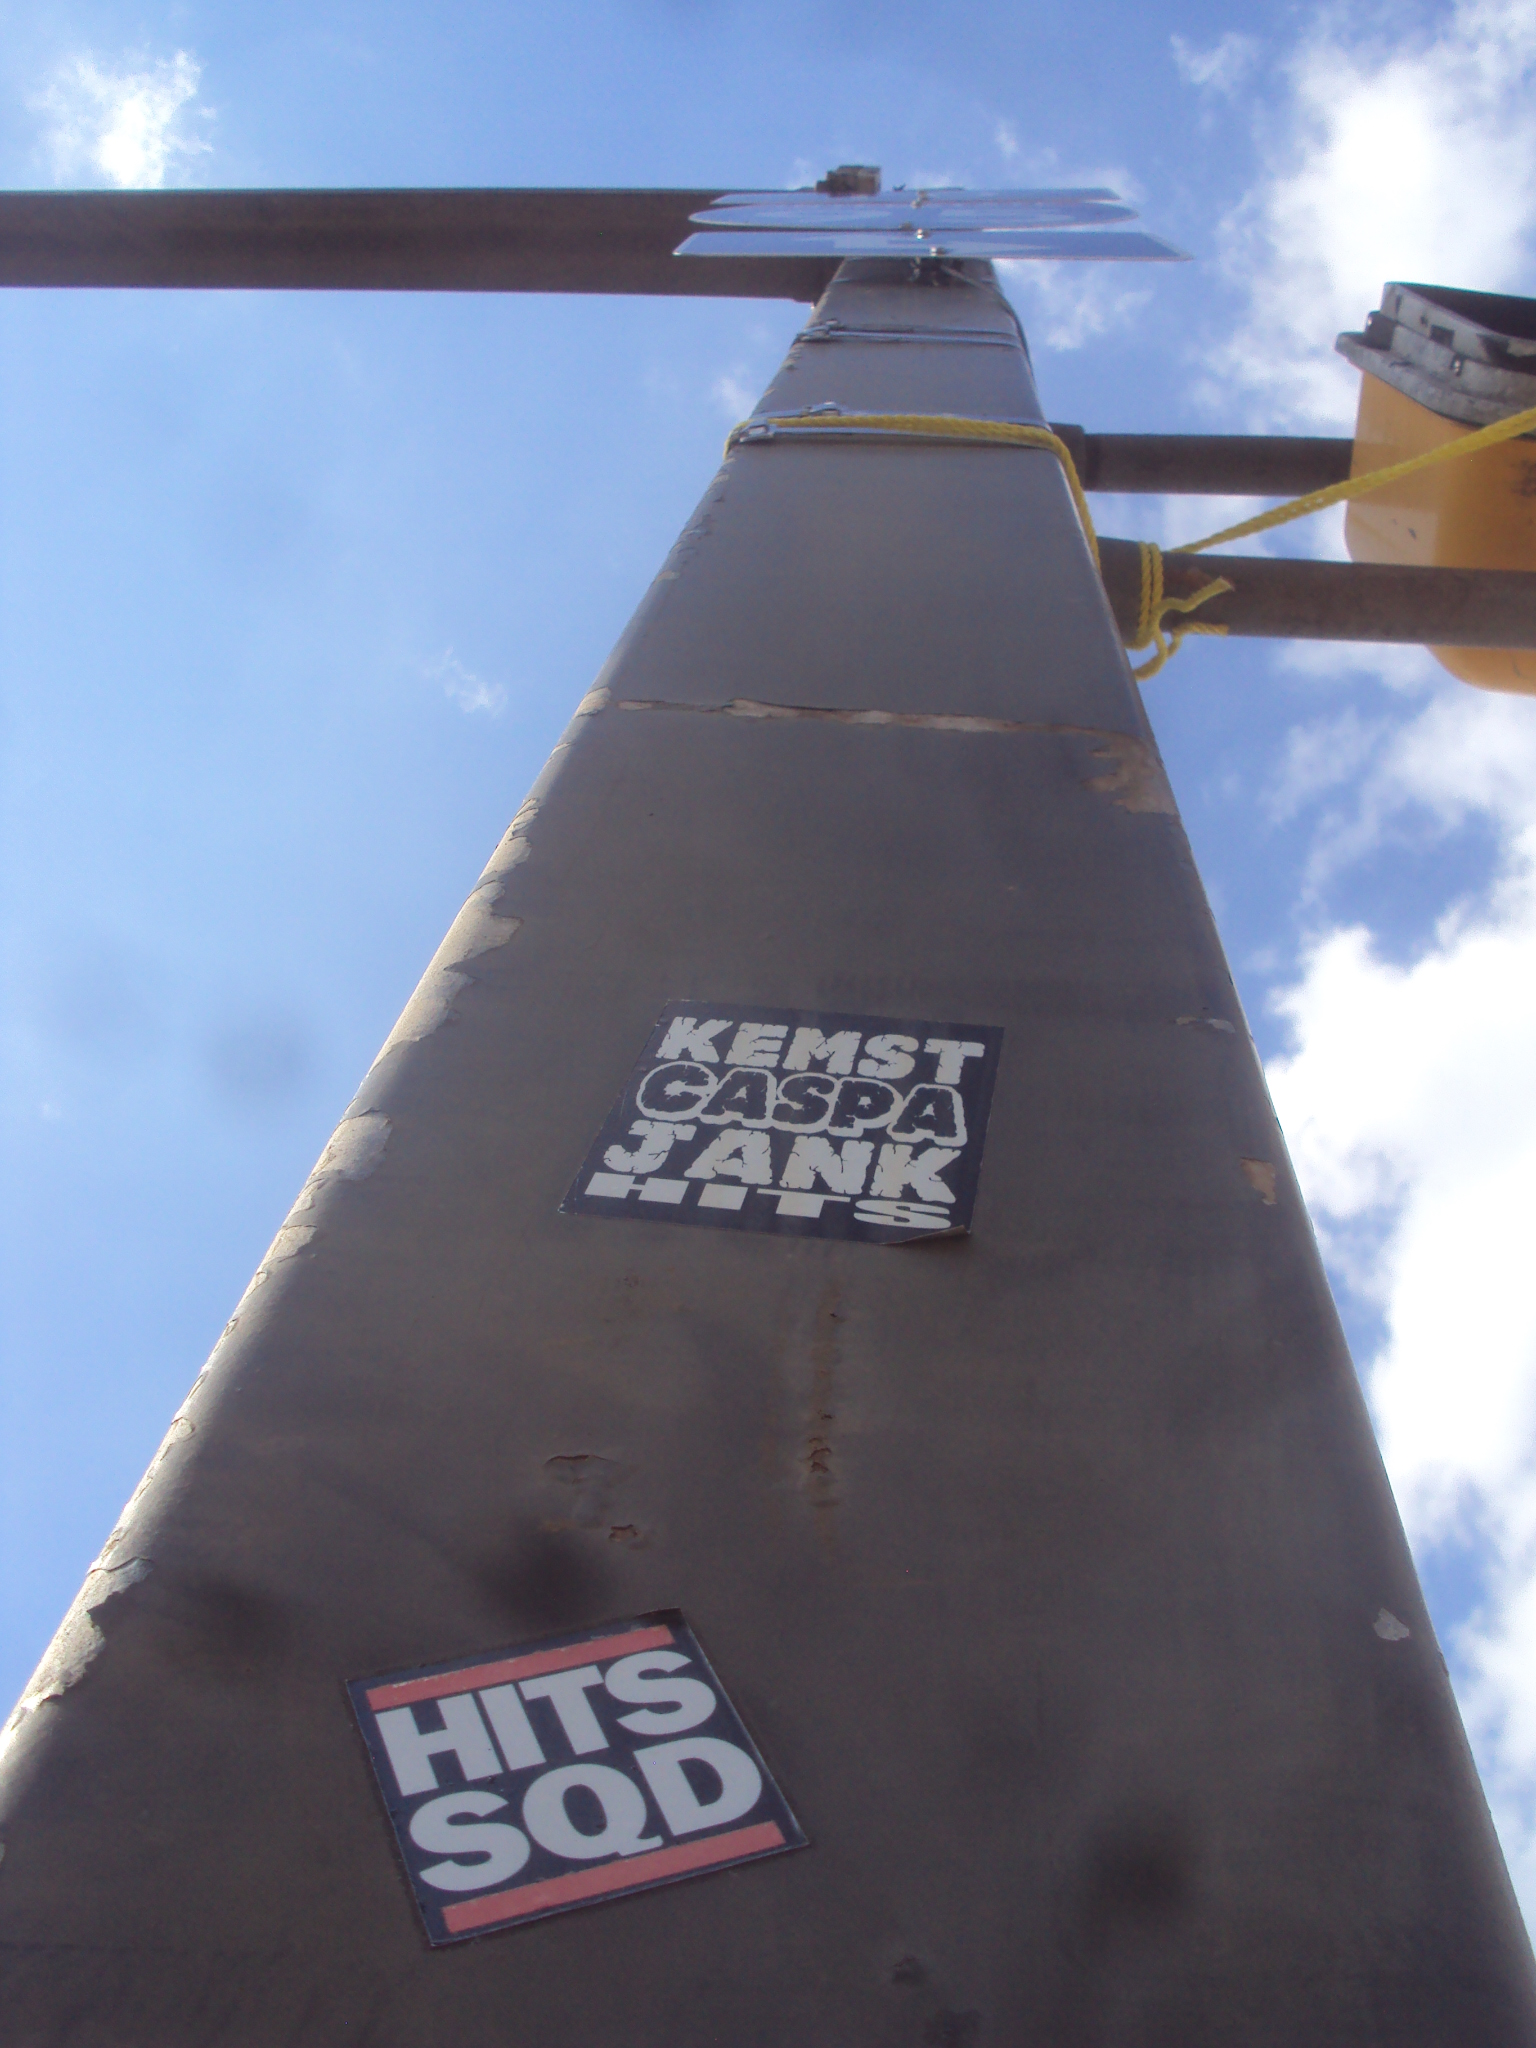
\includegraphics[height=4in]{portrait.jpg}

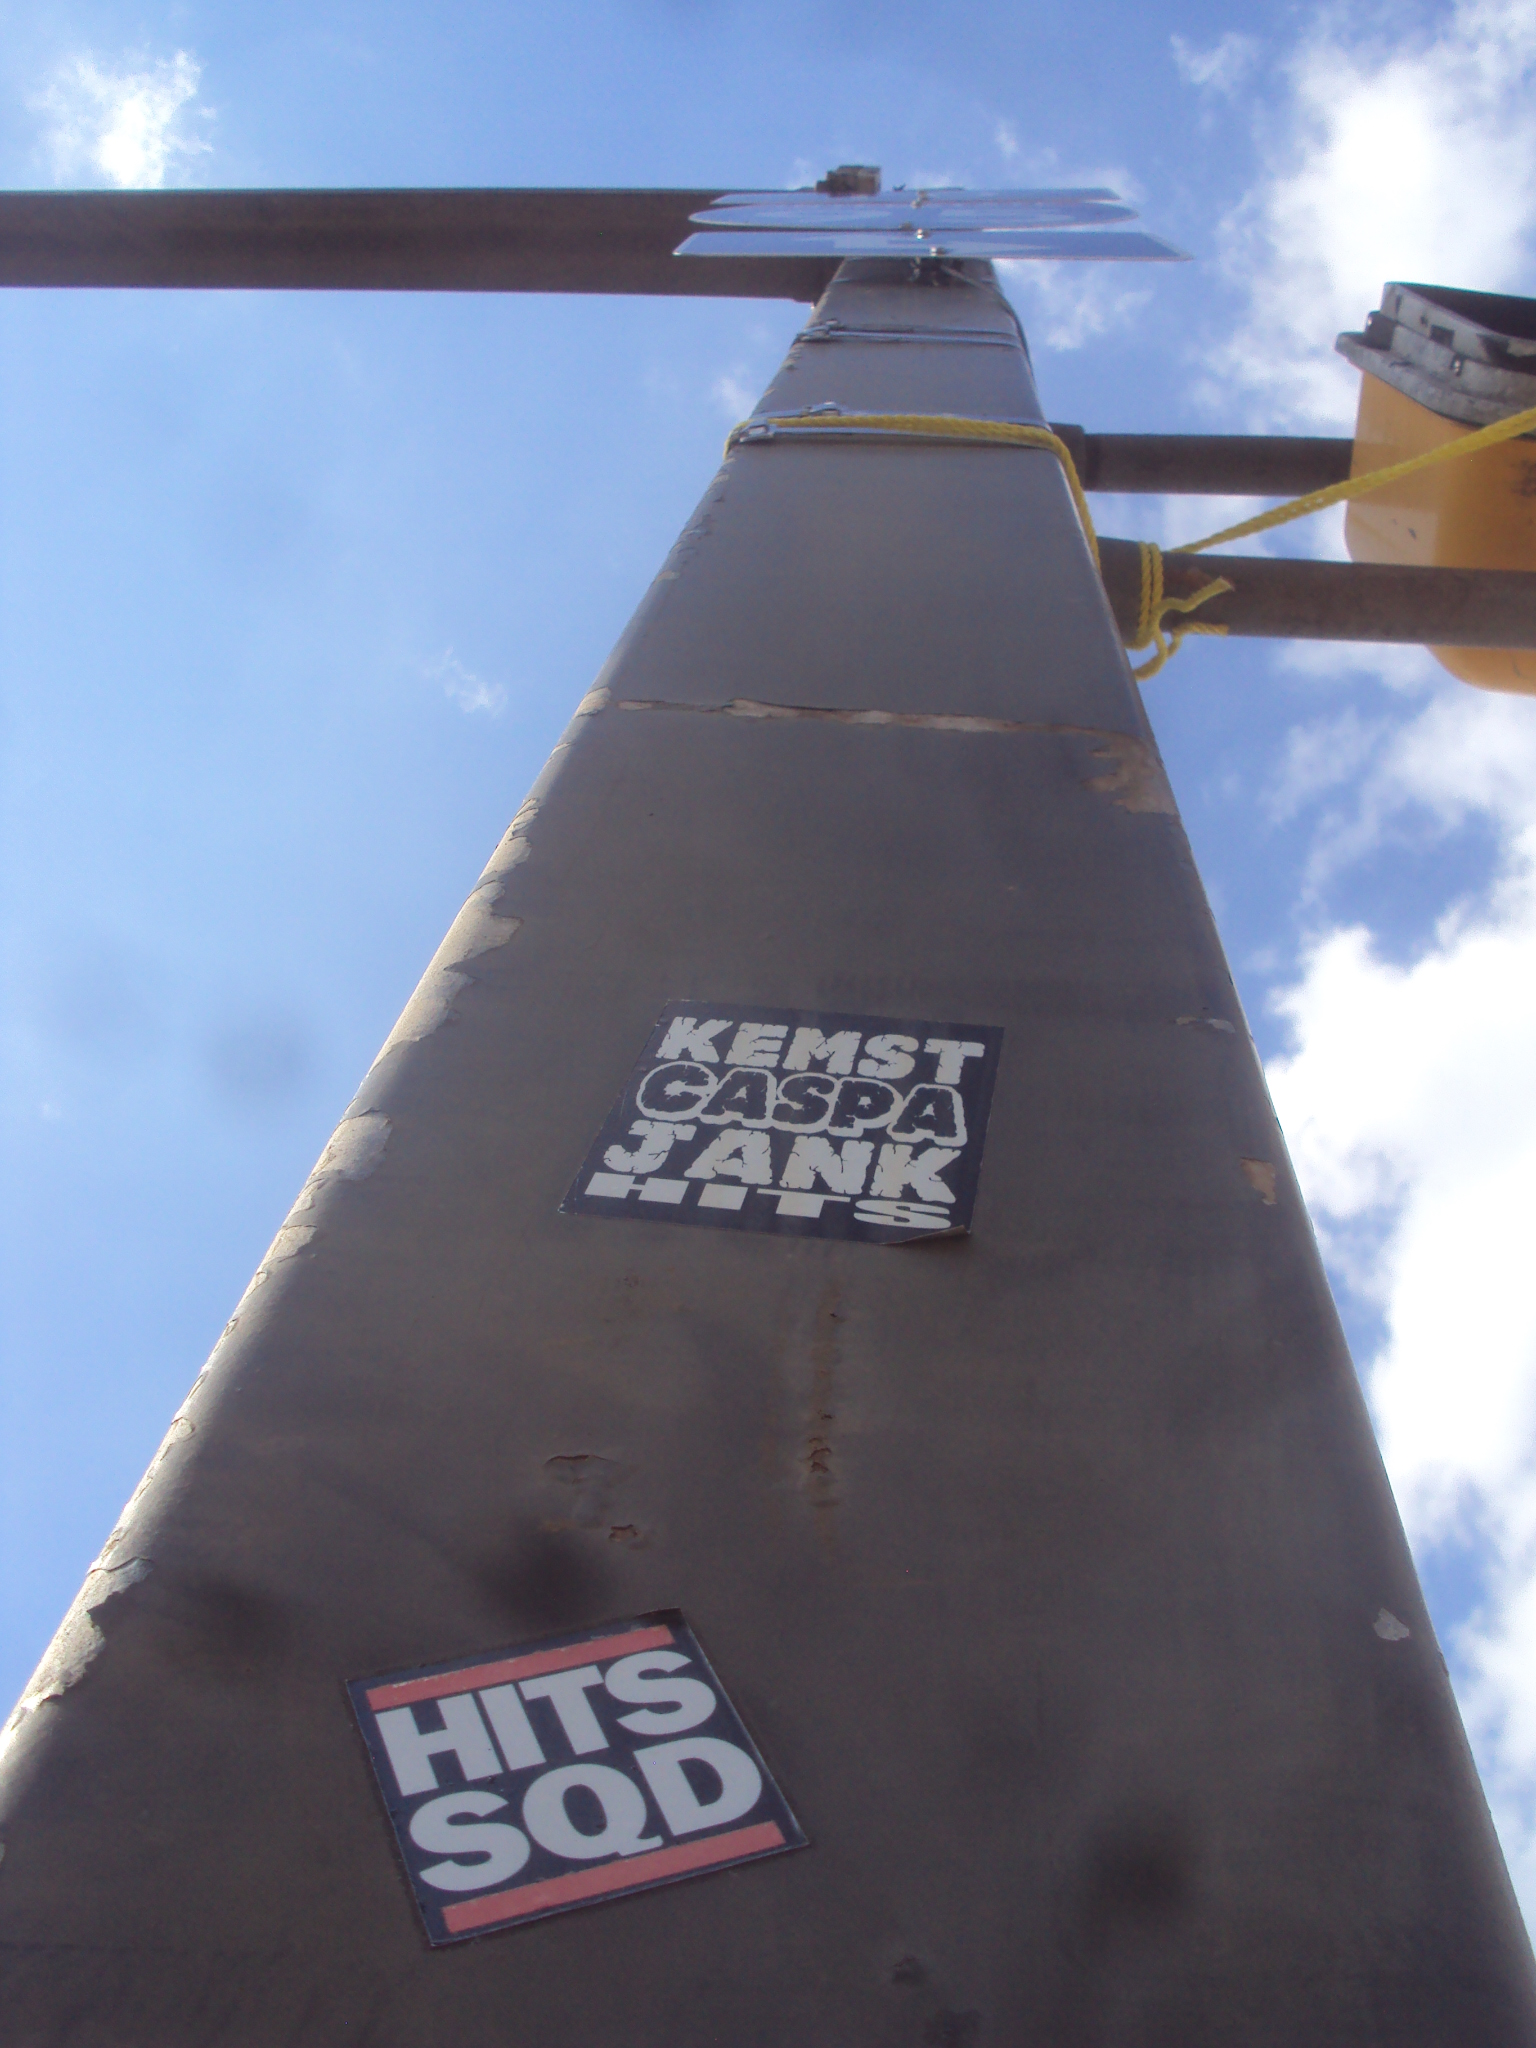
\includegraphics[height=4in]{portrait.jpg}

CAPTION P1\\
CAPTION P2\\
CAPTION P3\\
\pagebreak

% Layout PP
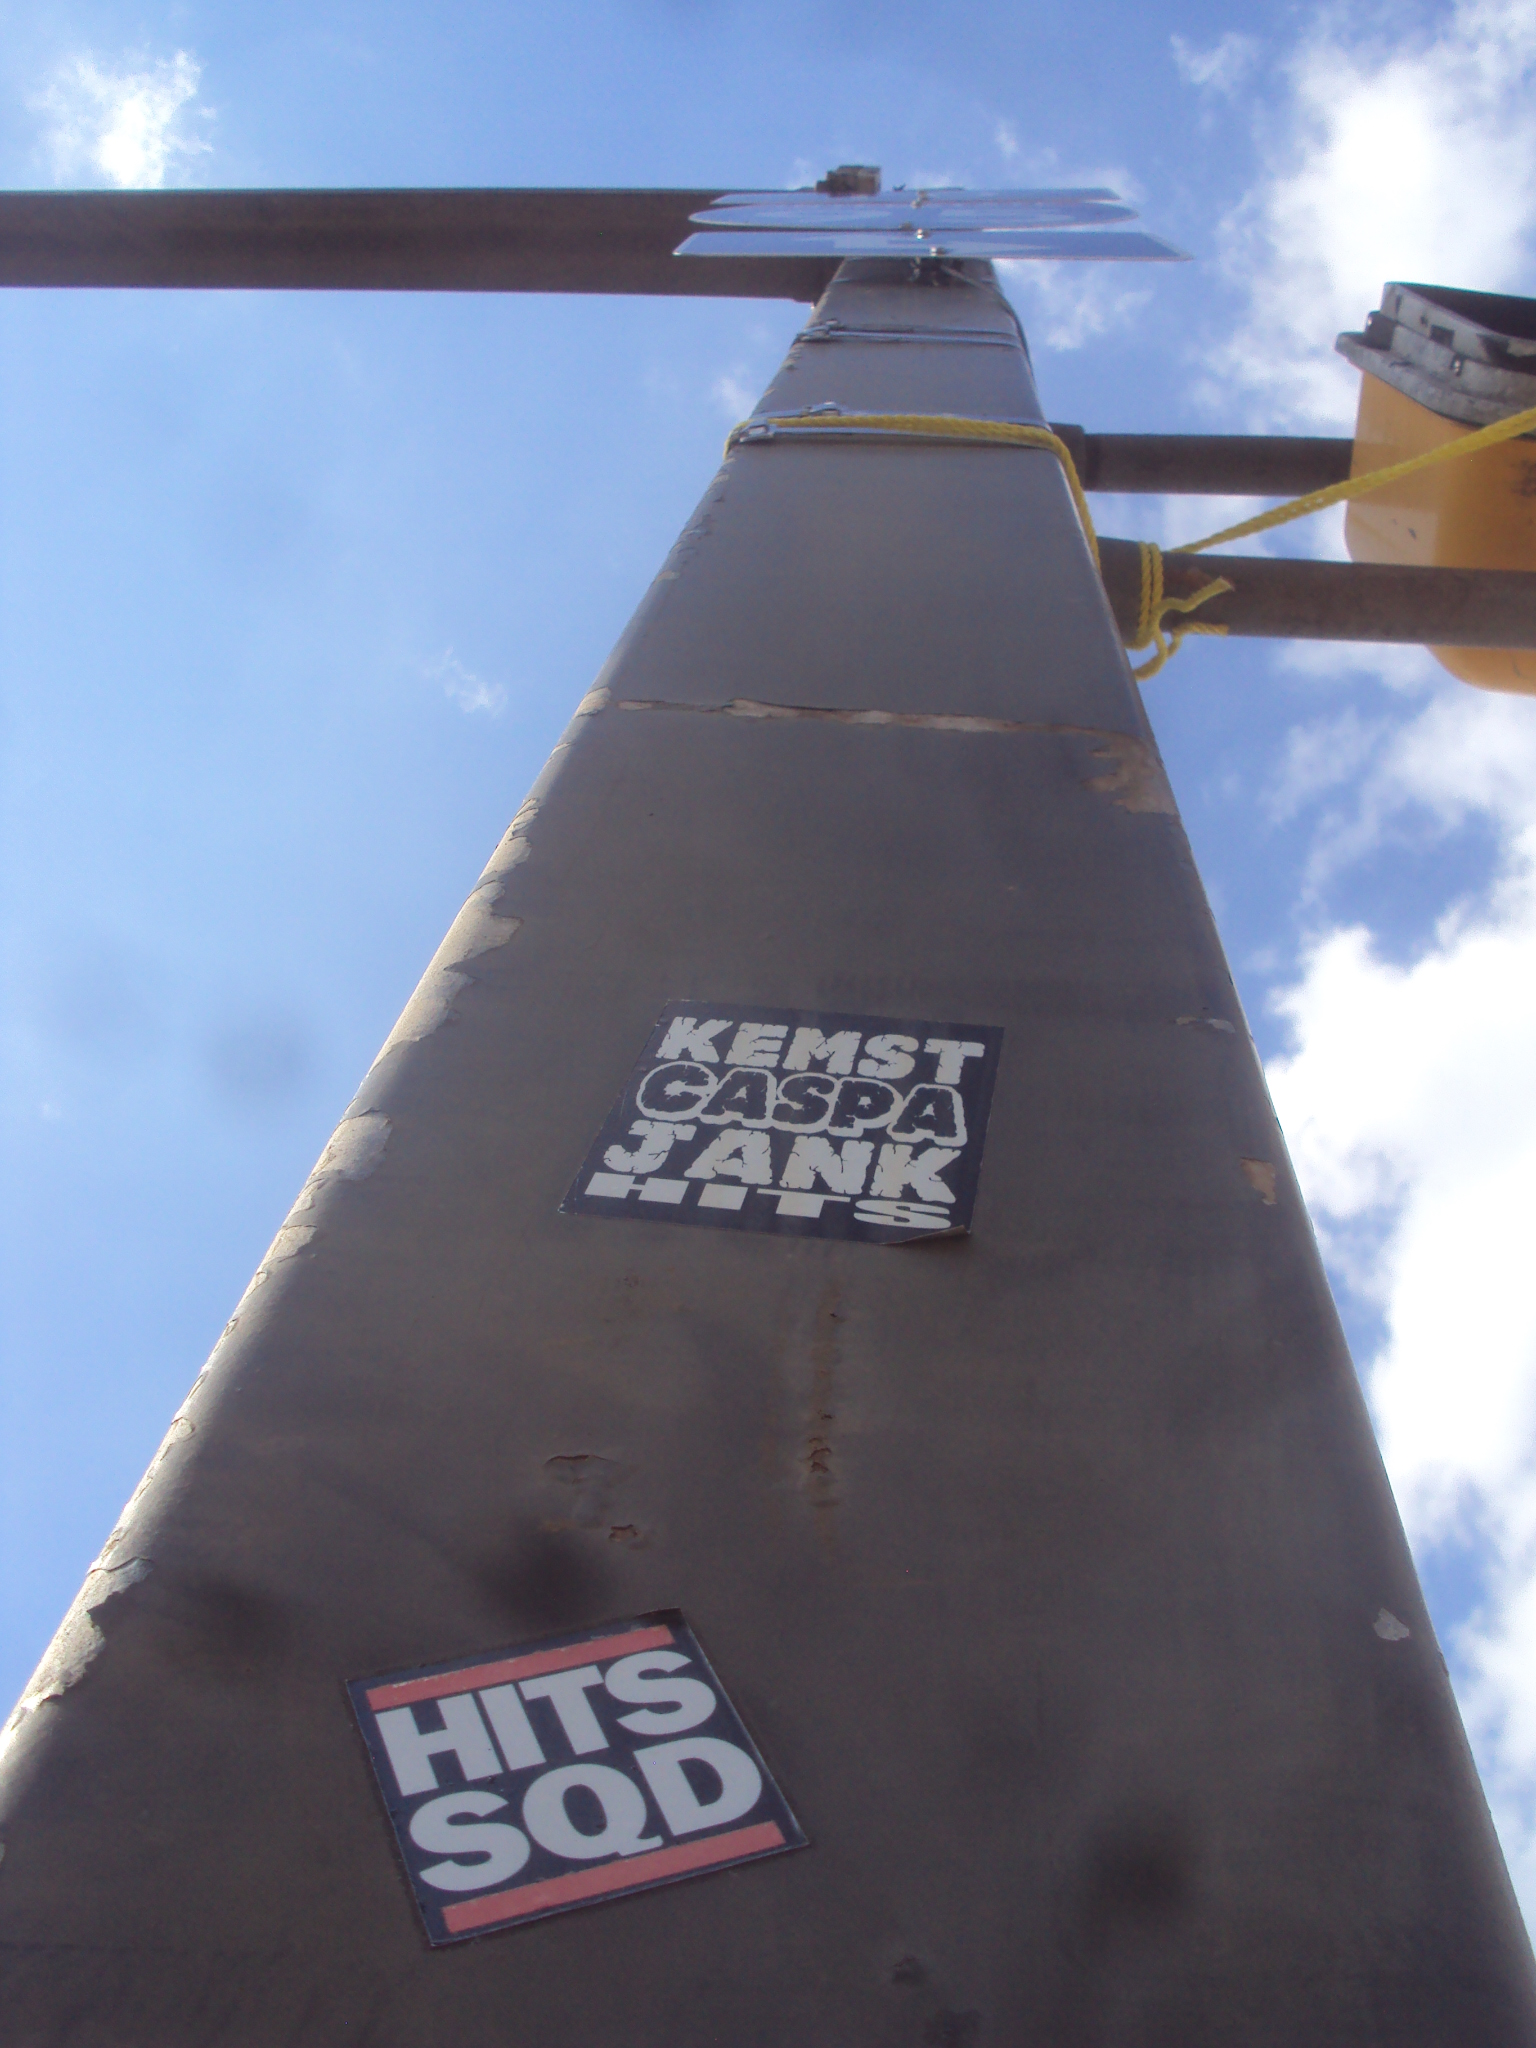
\includegraphics[height=4in]{portrait.jpg}
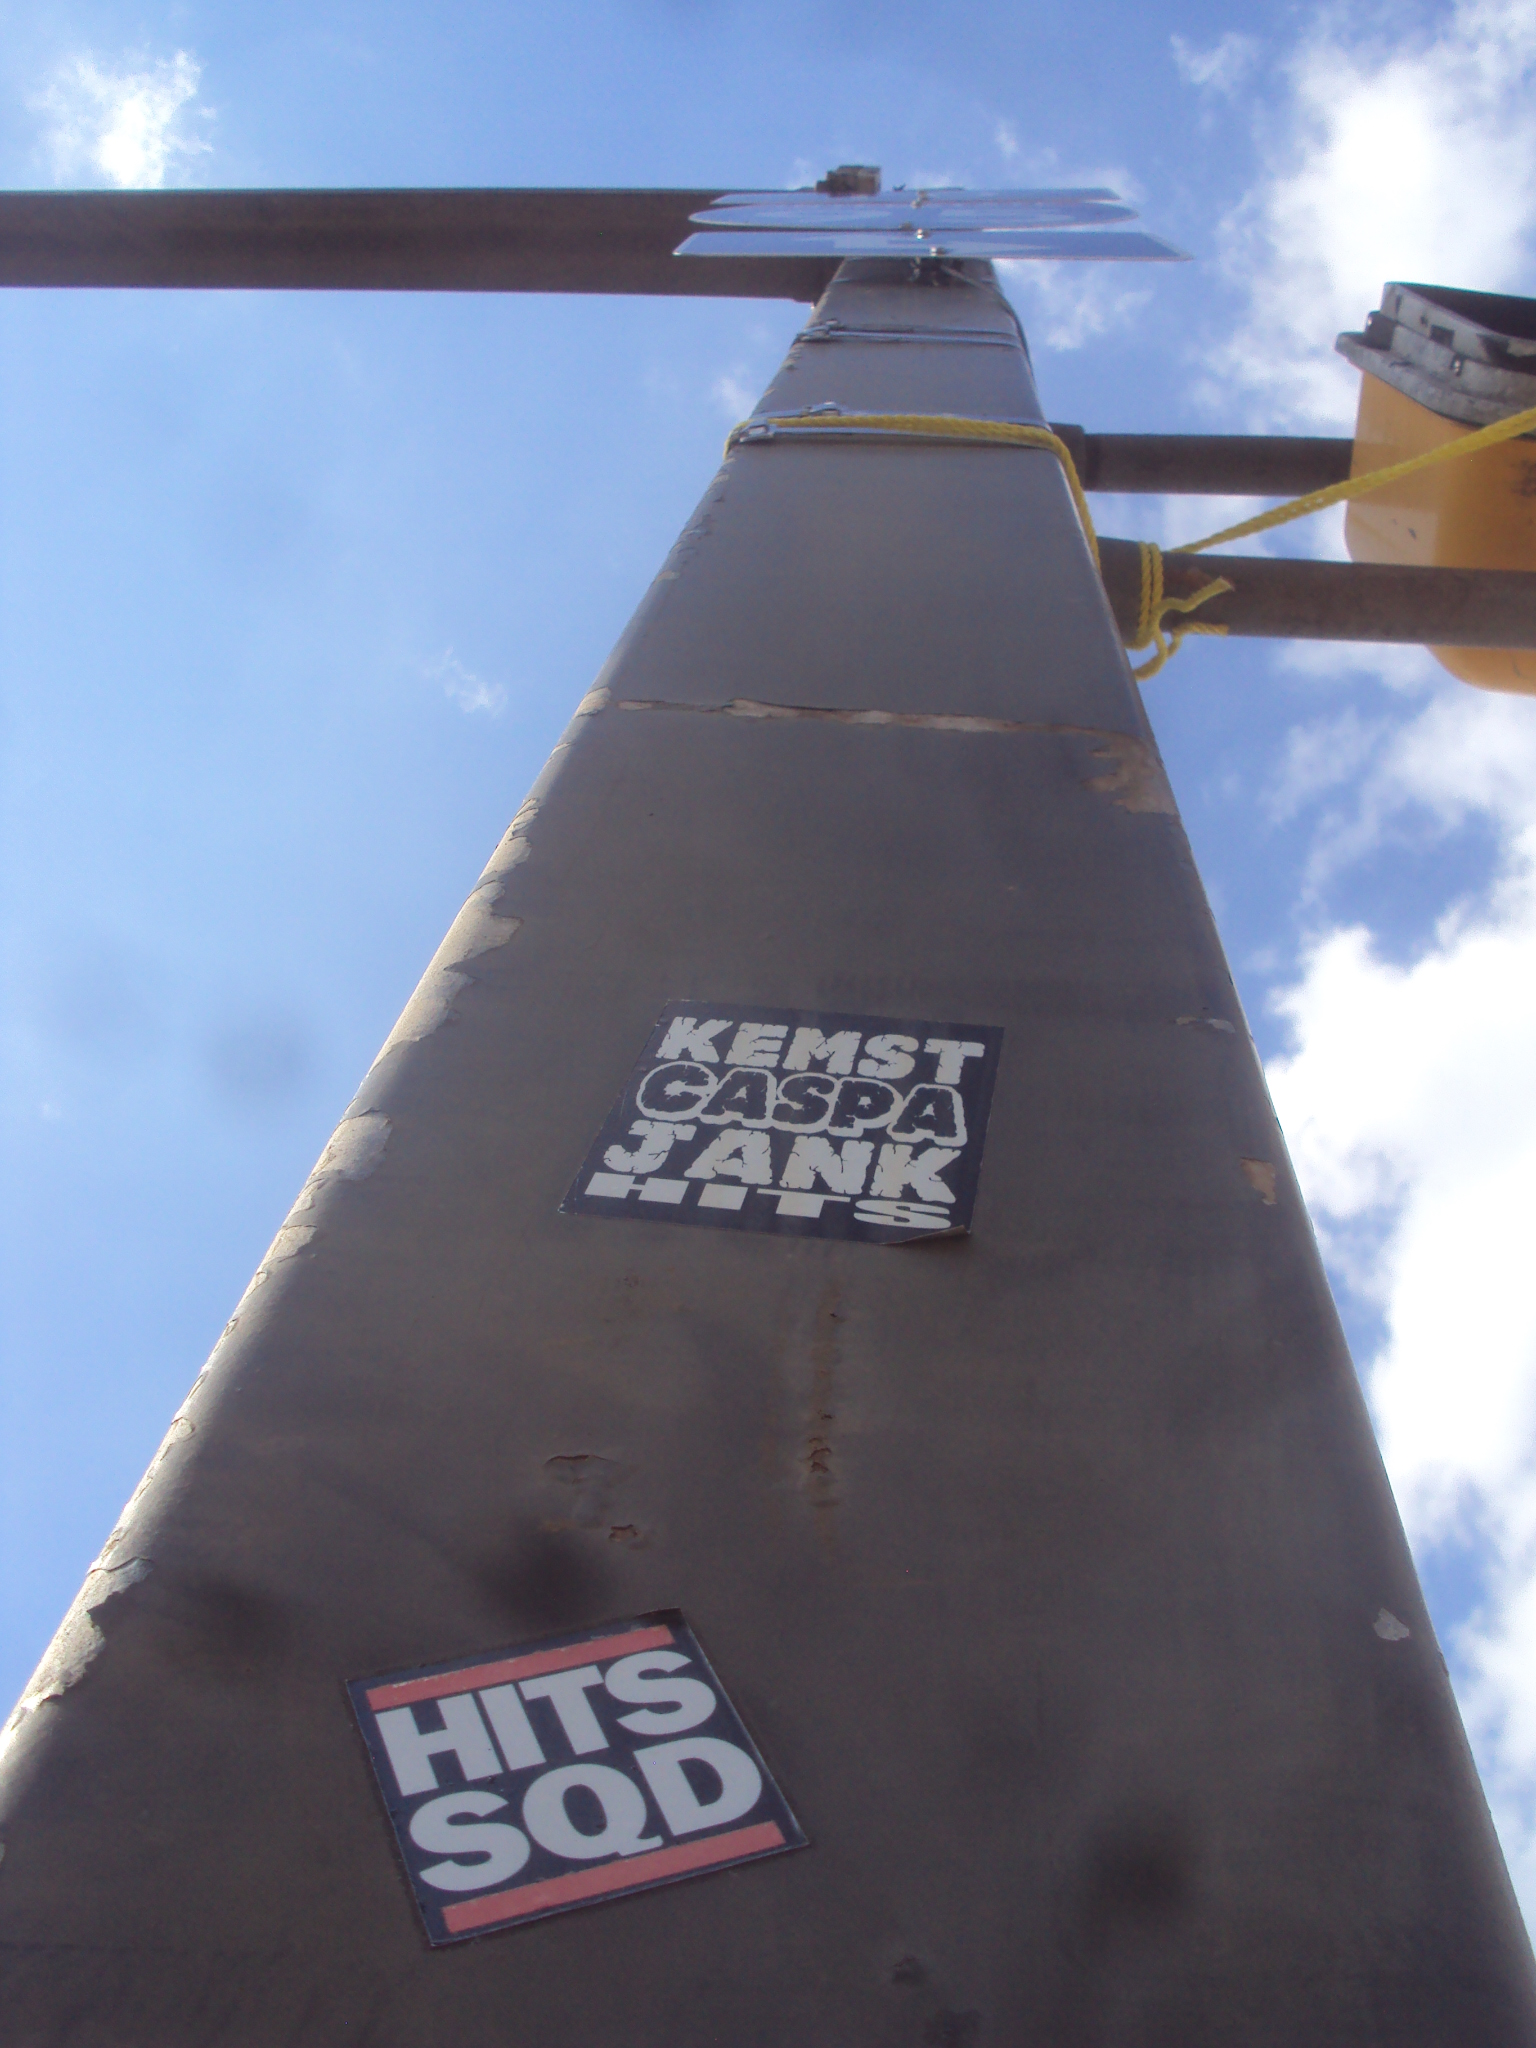
\includegraphics[height=4in]{portrait.jpg}

CAPTION P1\\
CAPTION P2\\
\pagebreak

% Layout P
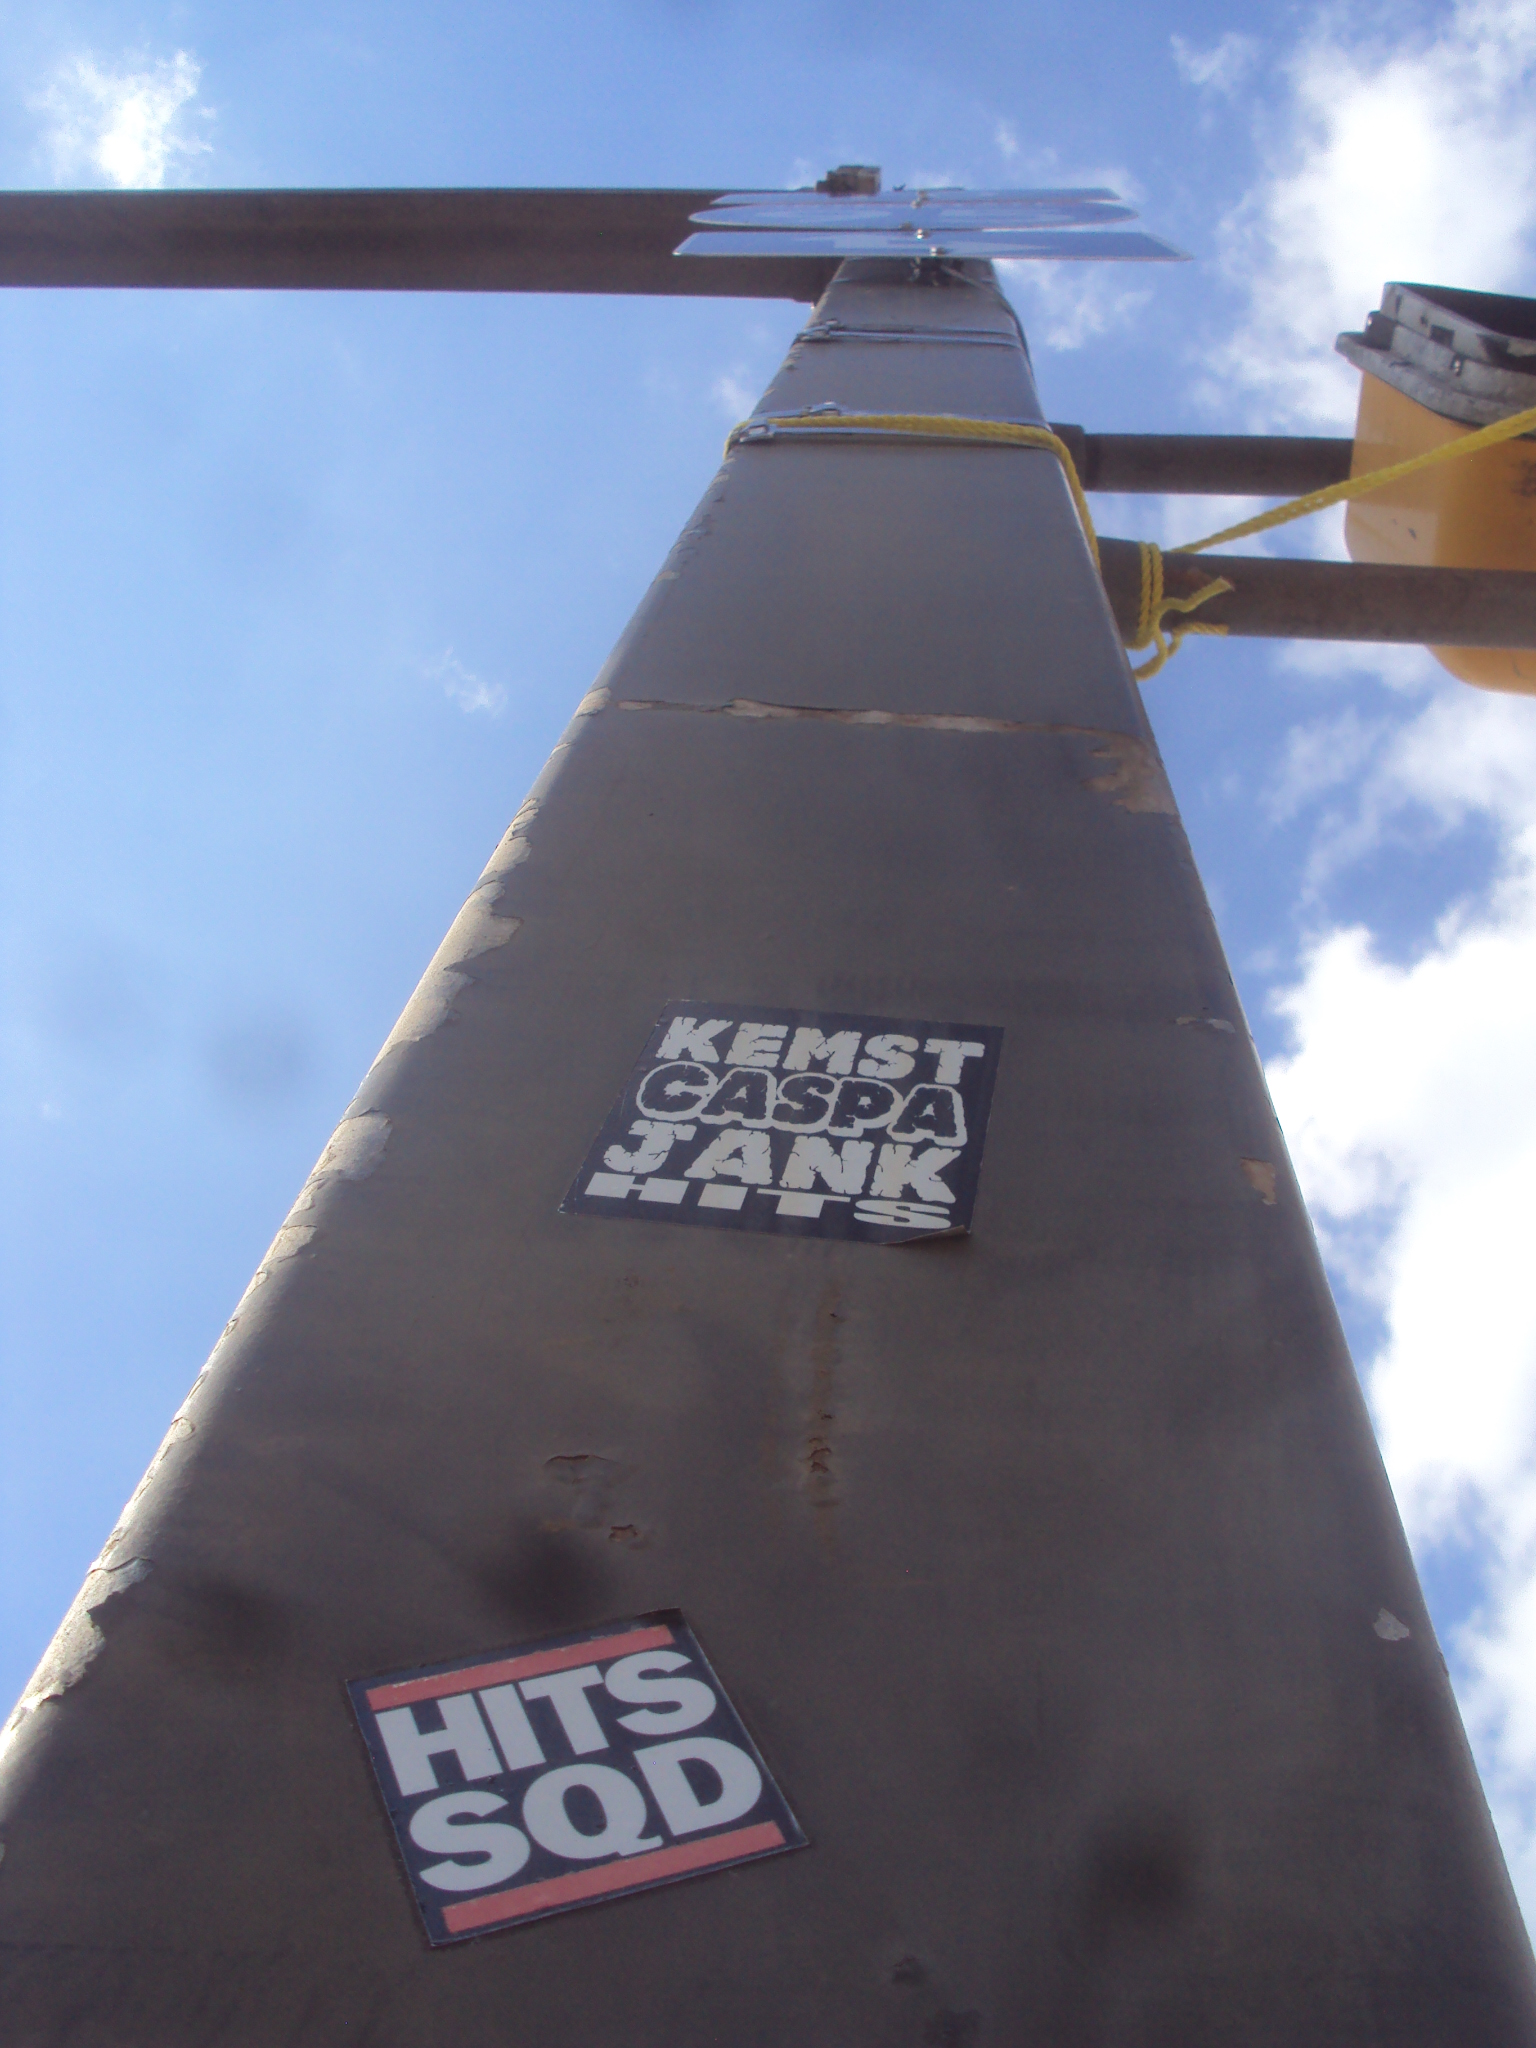
\includegraphics[height=4in]{portrait.jpg}

CAPTION P1\\
\pagebreak

% Layout PPL
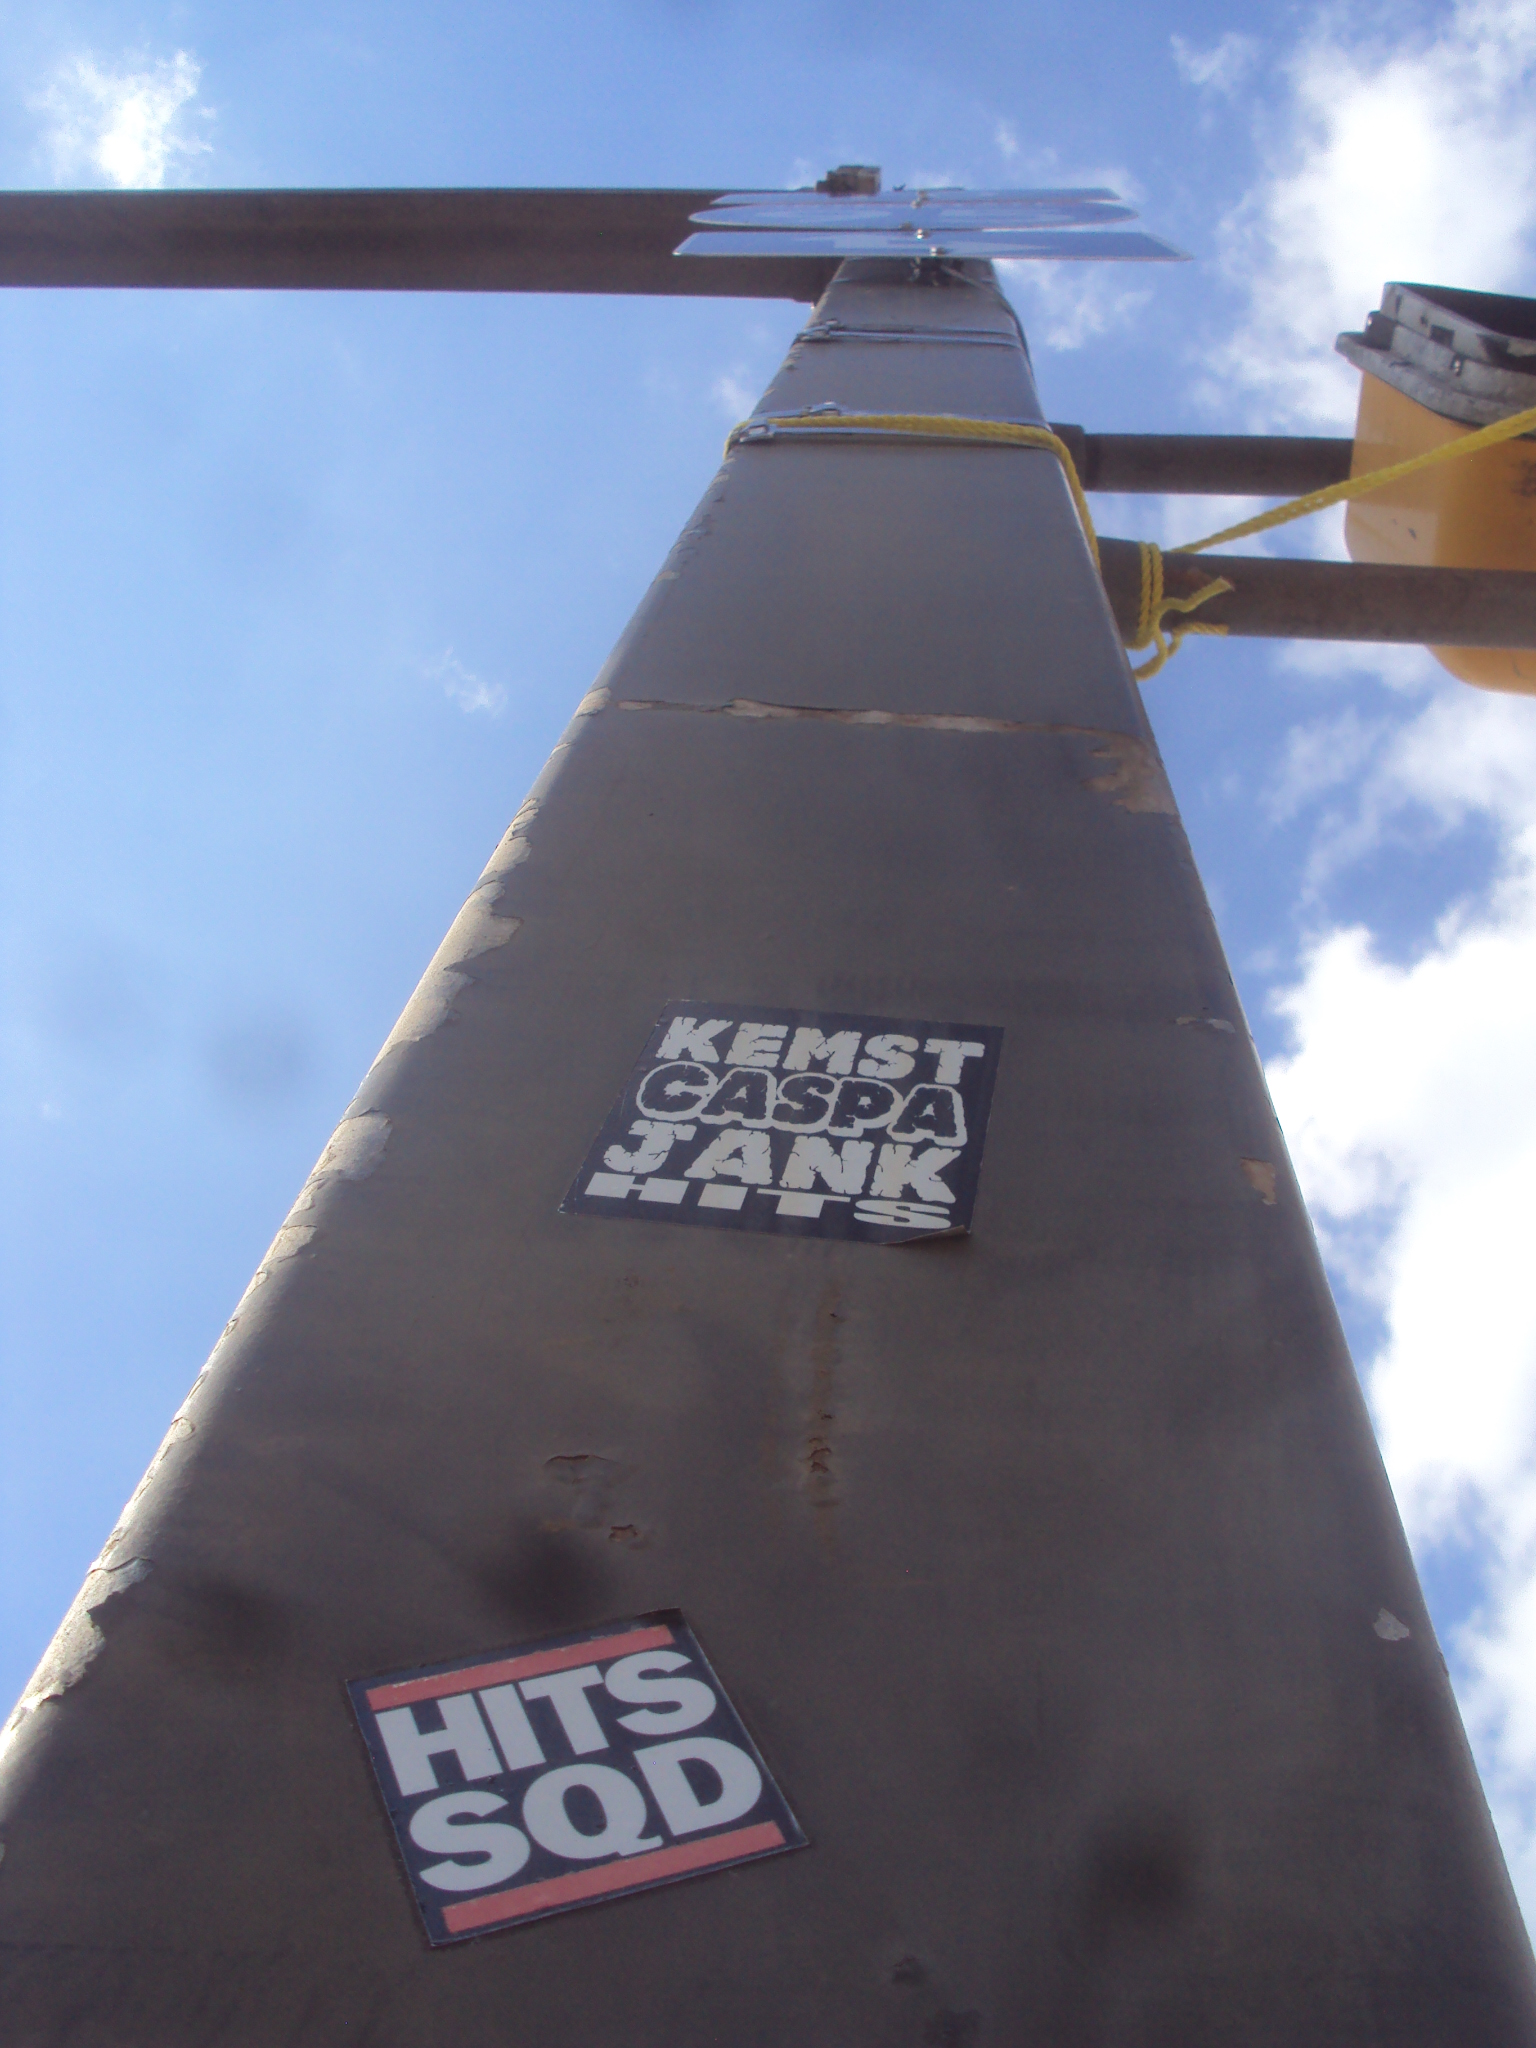
\includegraphics[height=4in]{portrait.jpg}
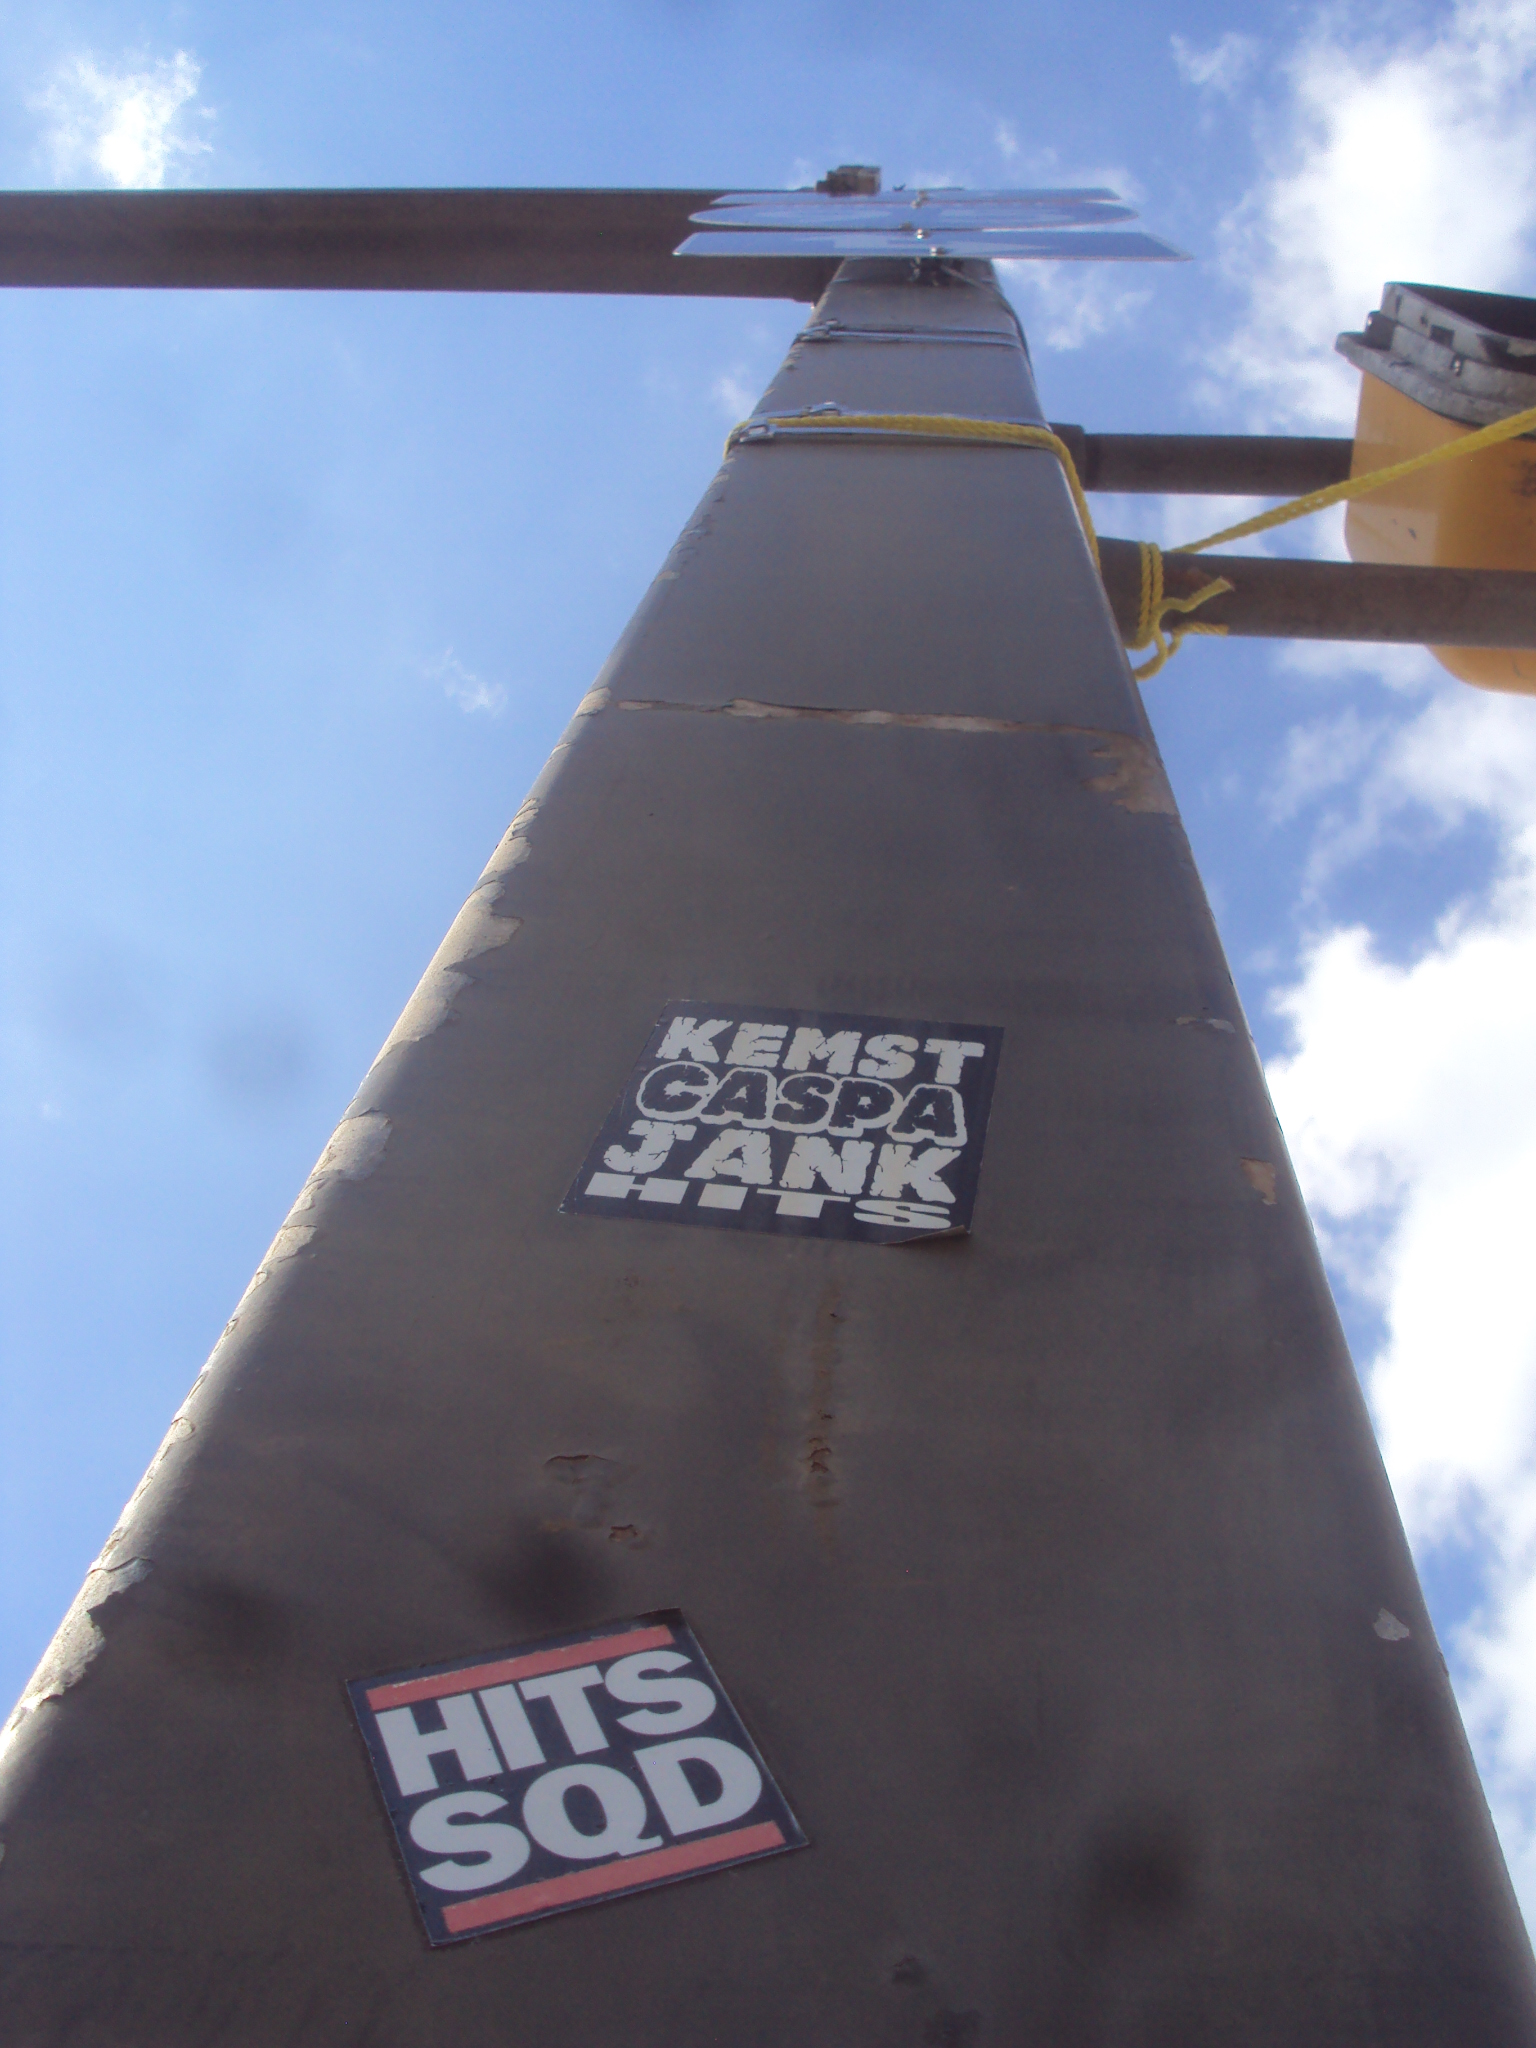
\includegraphics[height=4in]{portrait.jpg}

\vspace{0.25in}
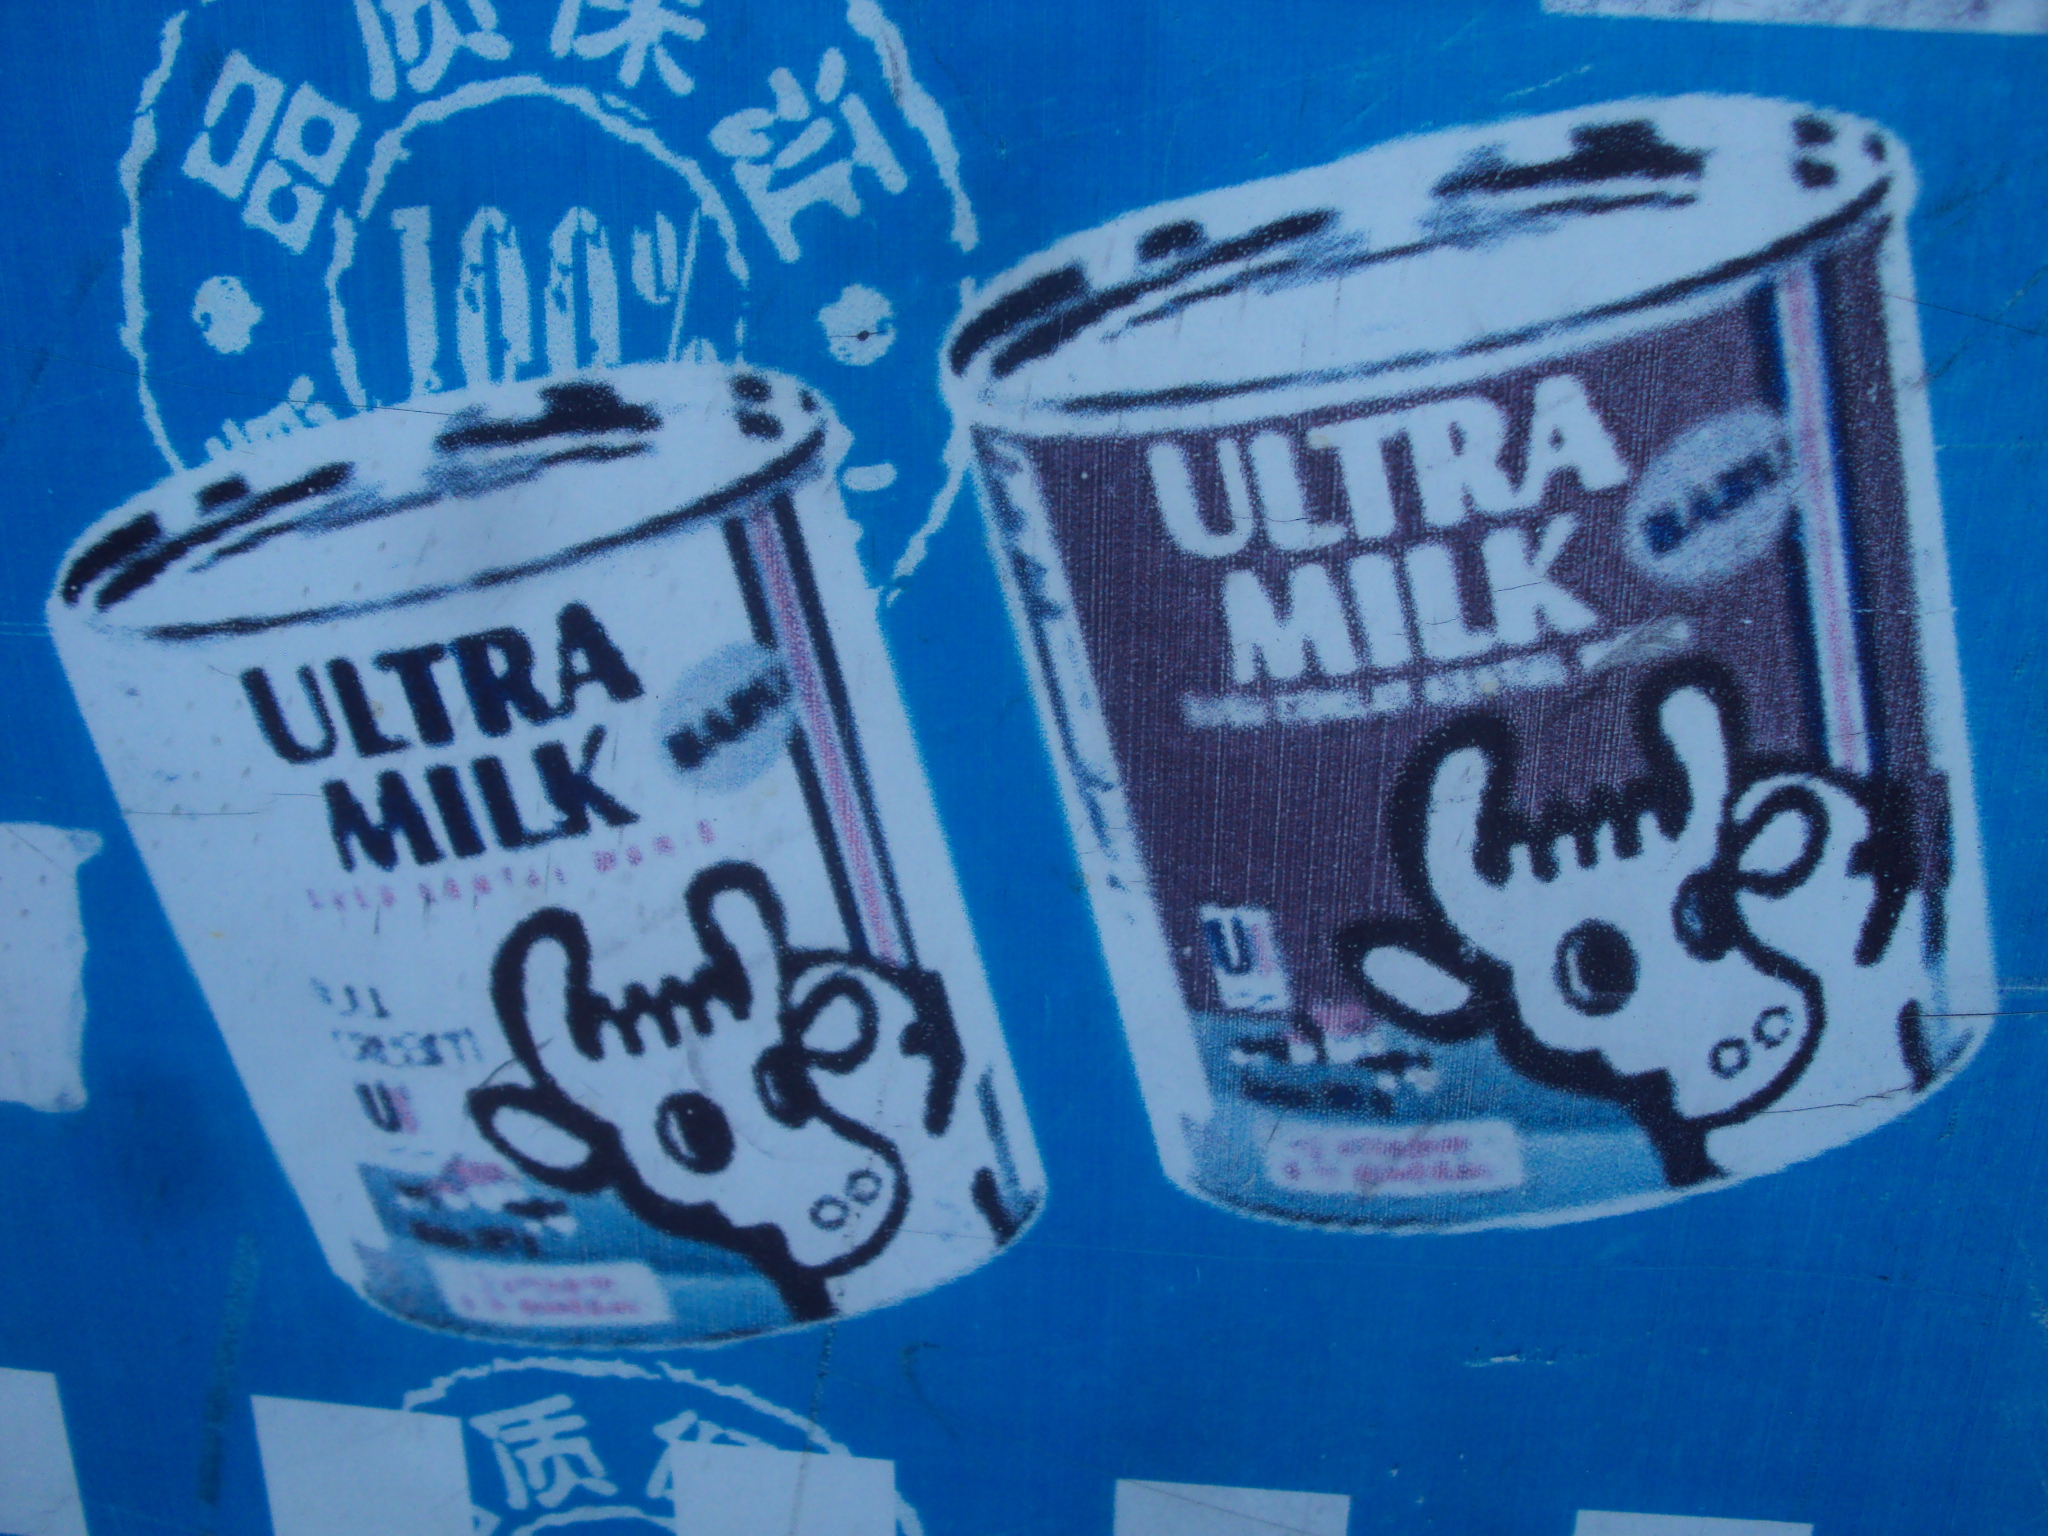
\includegraphics[width=5.19in]{landscape.jpg}

CAPTION P1\\
CAPTION P2\\
CAPTION L1\\
\pagebreak

% Layout LPP
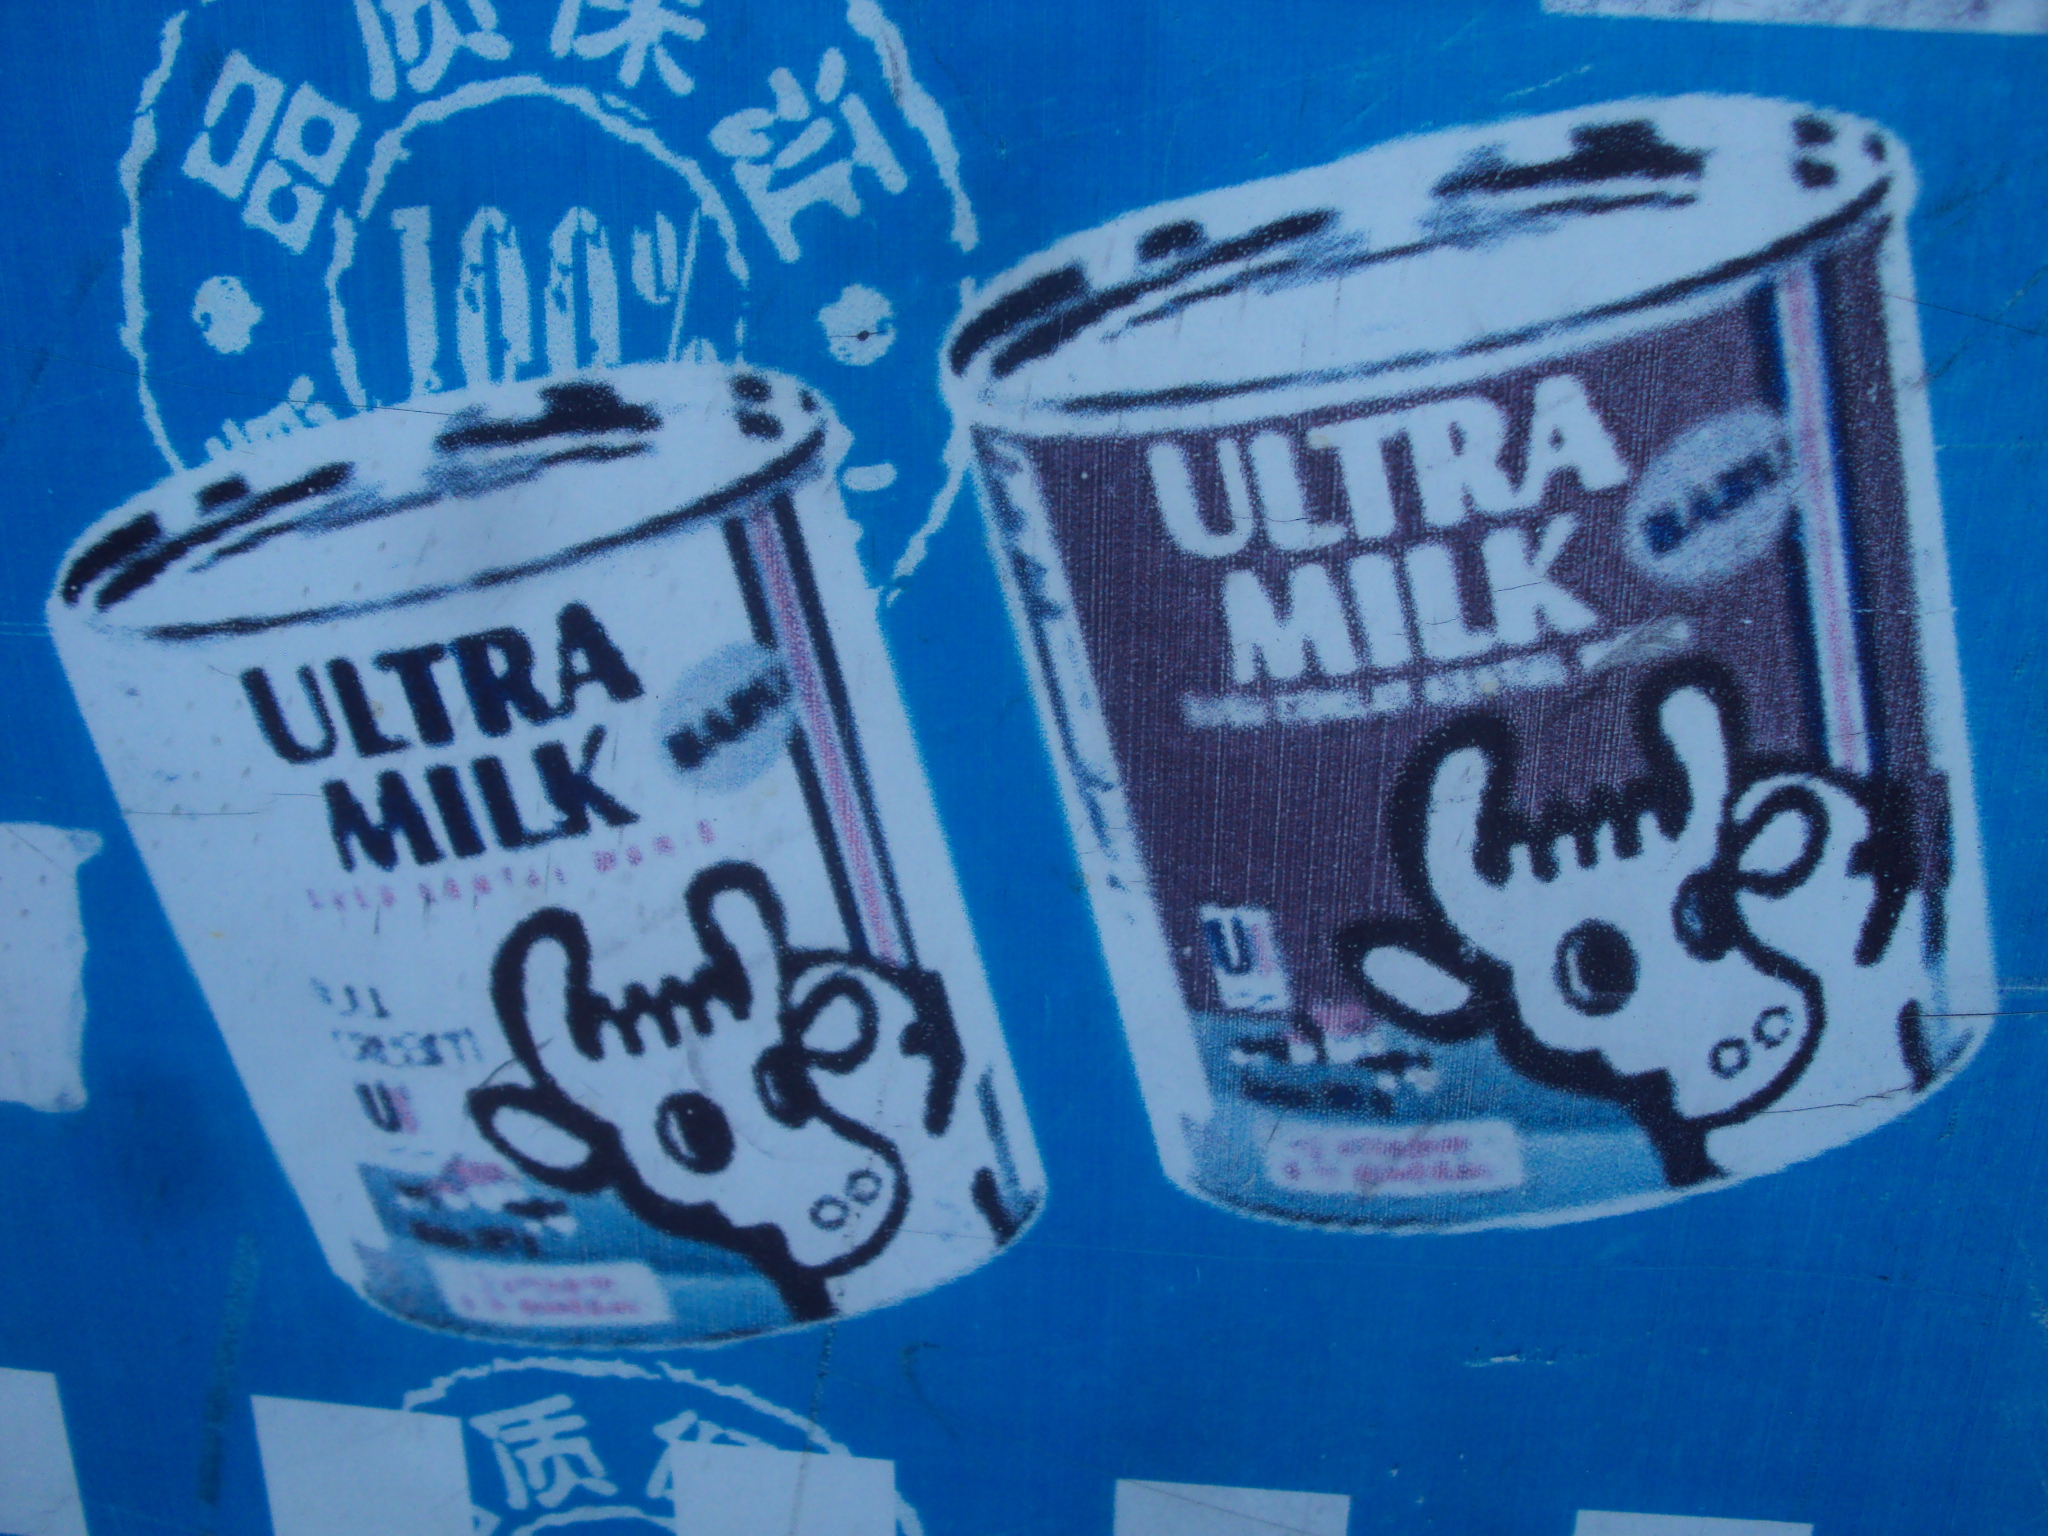
\includegraphics[width=5.19in]{landscape.jpg}

\vspace{0.25in}
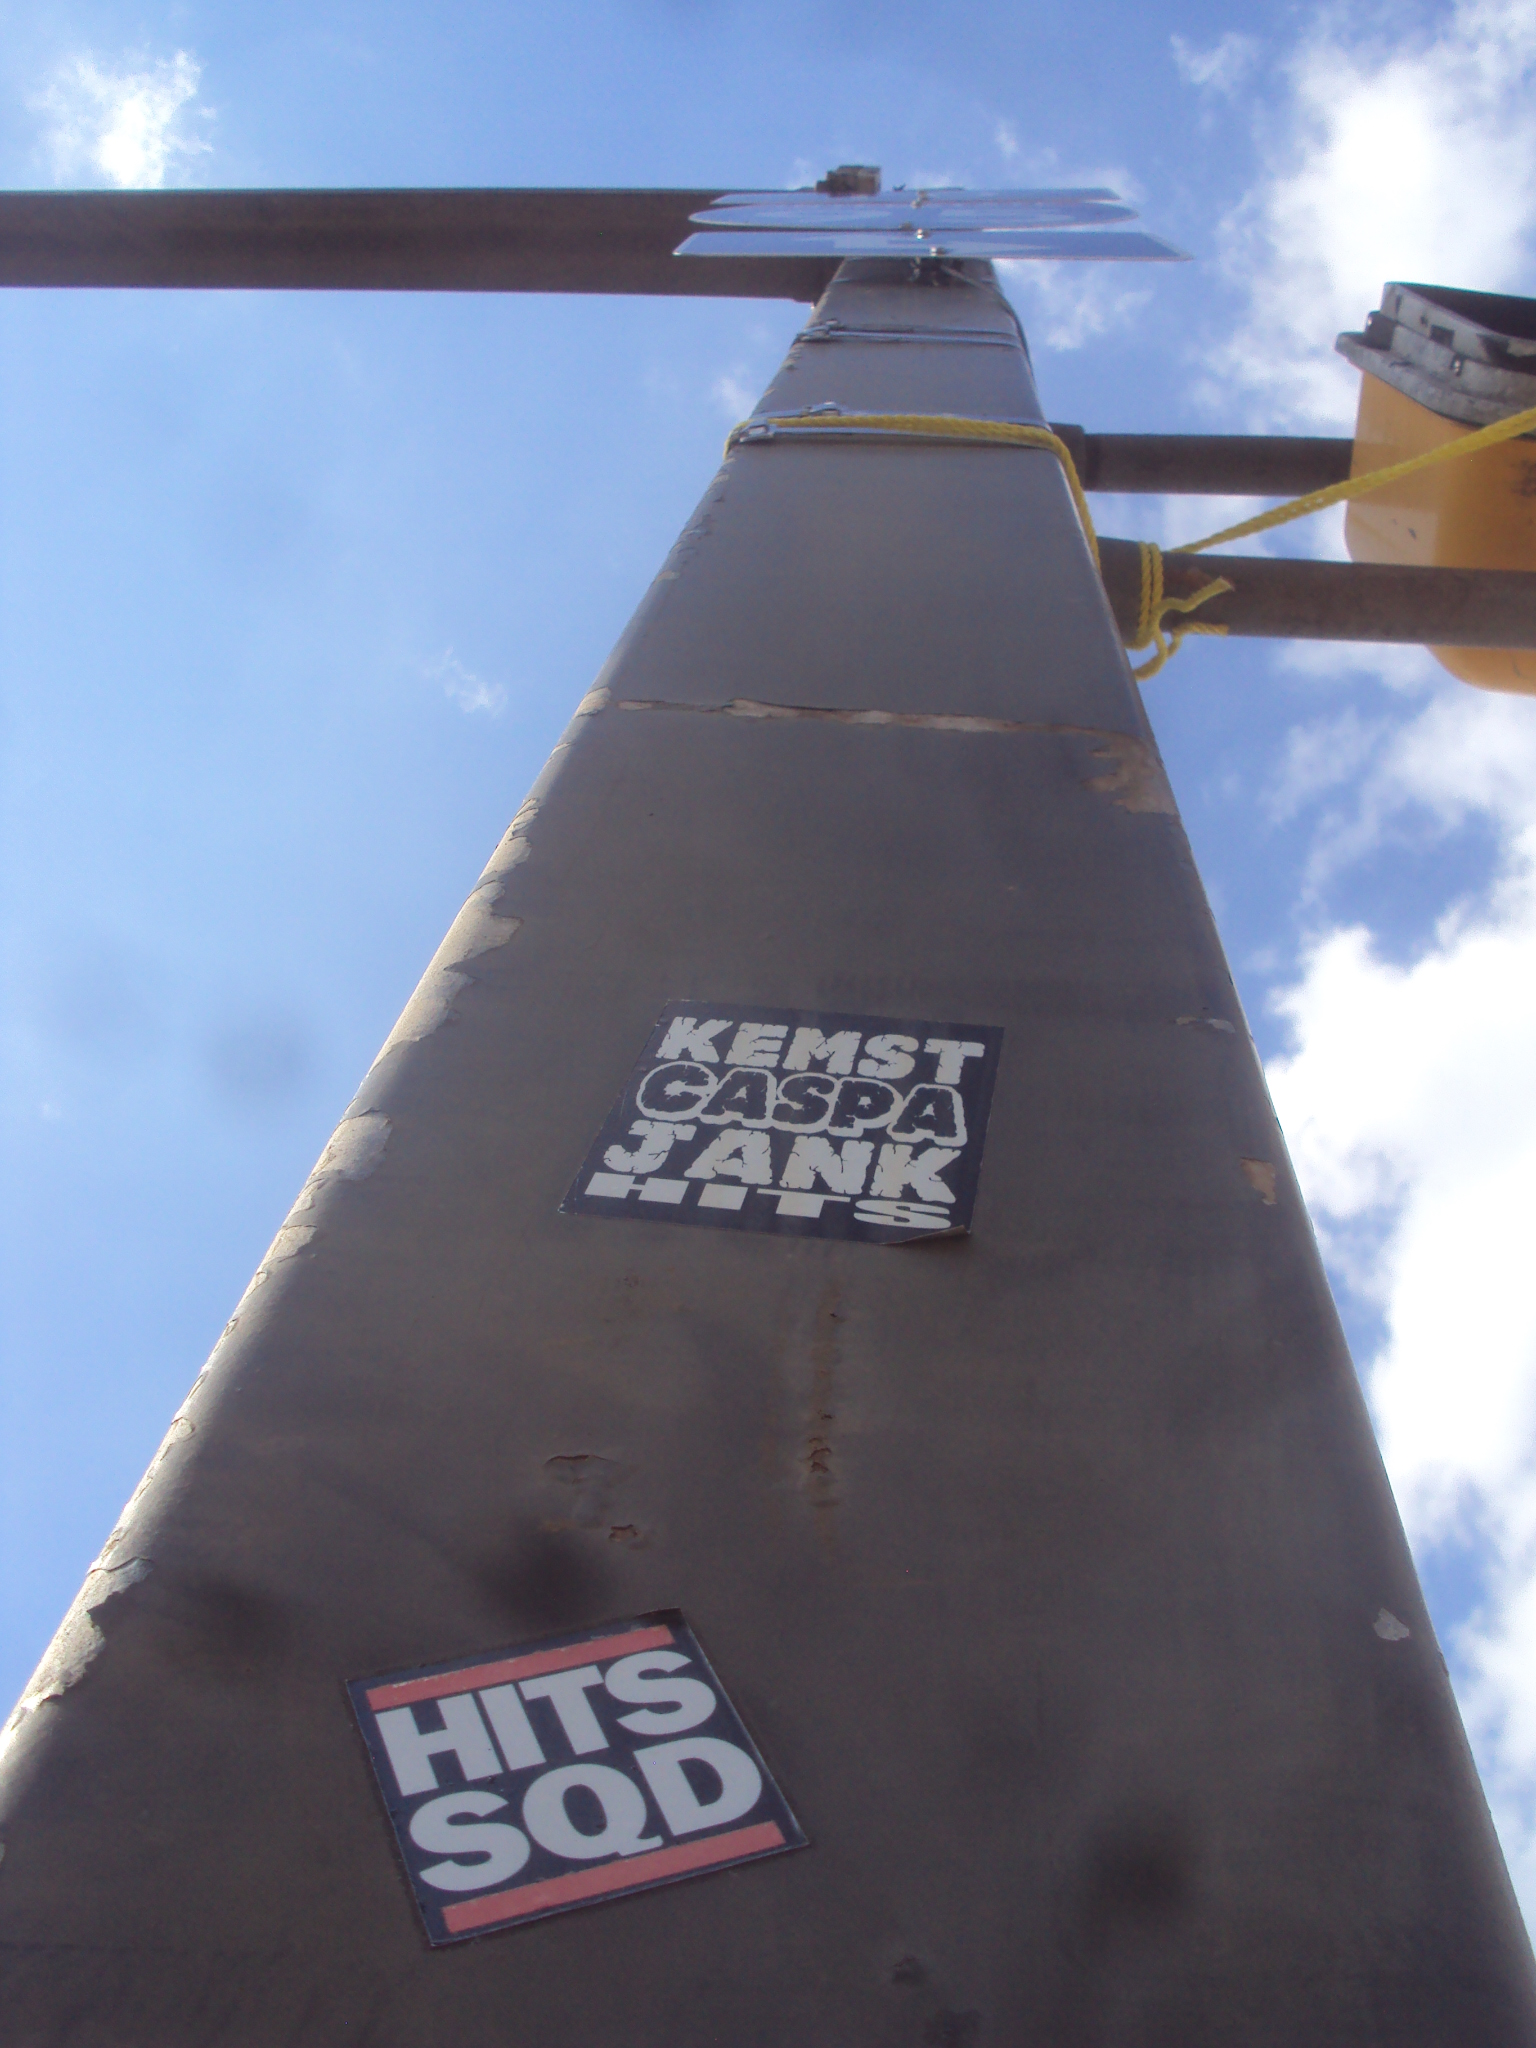
\includegraphics[height=4in]{portrait.jpg}
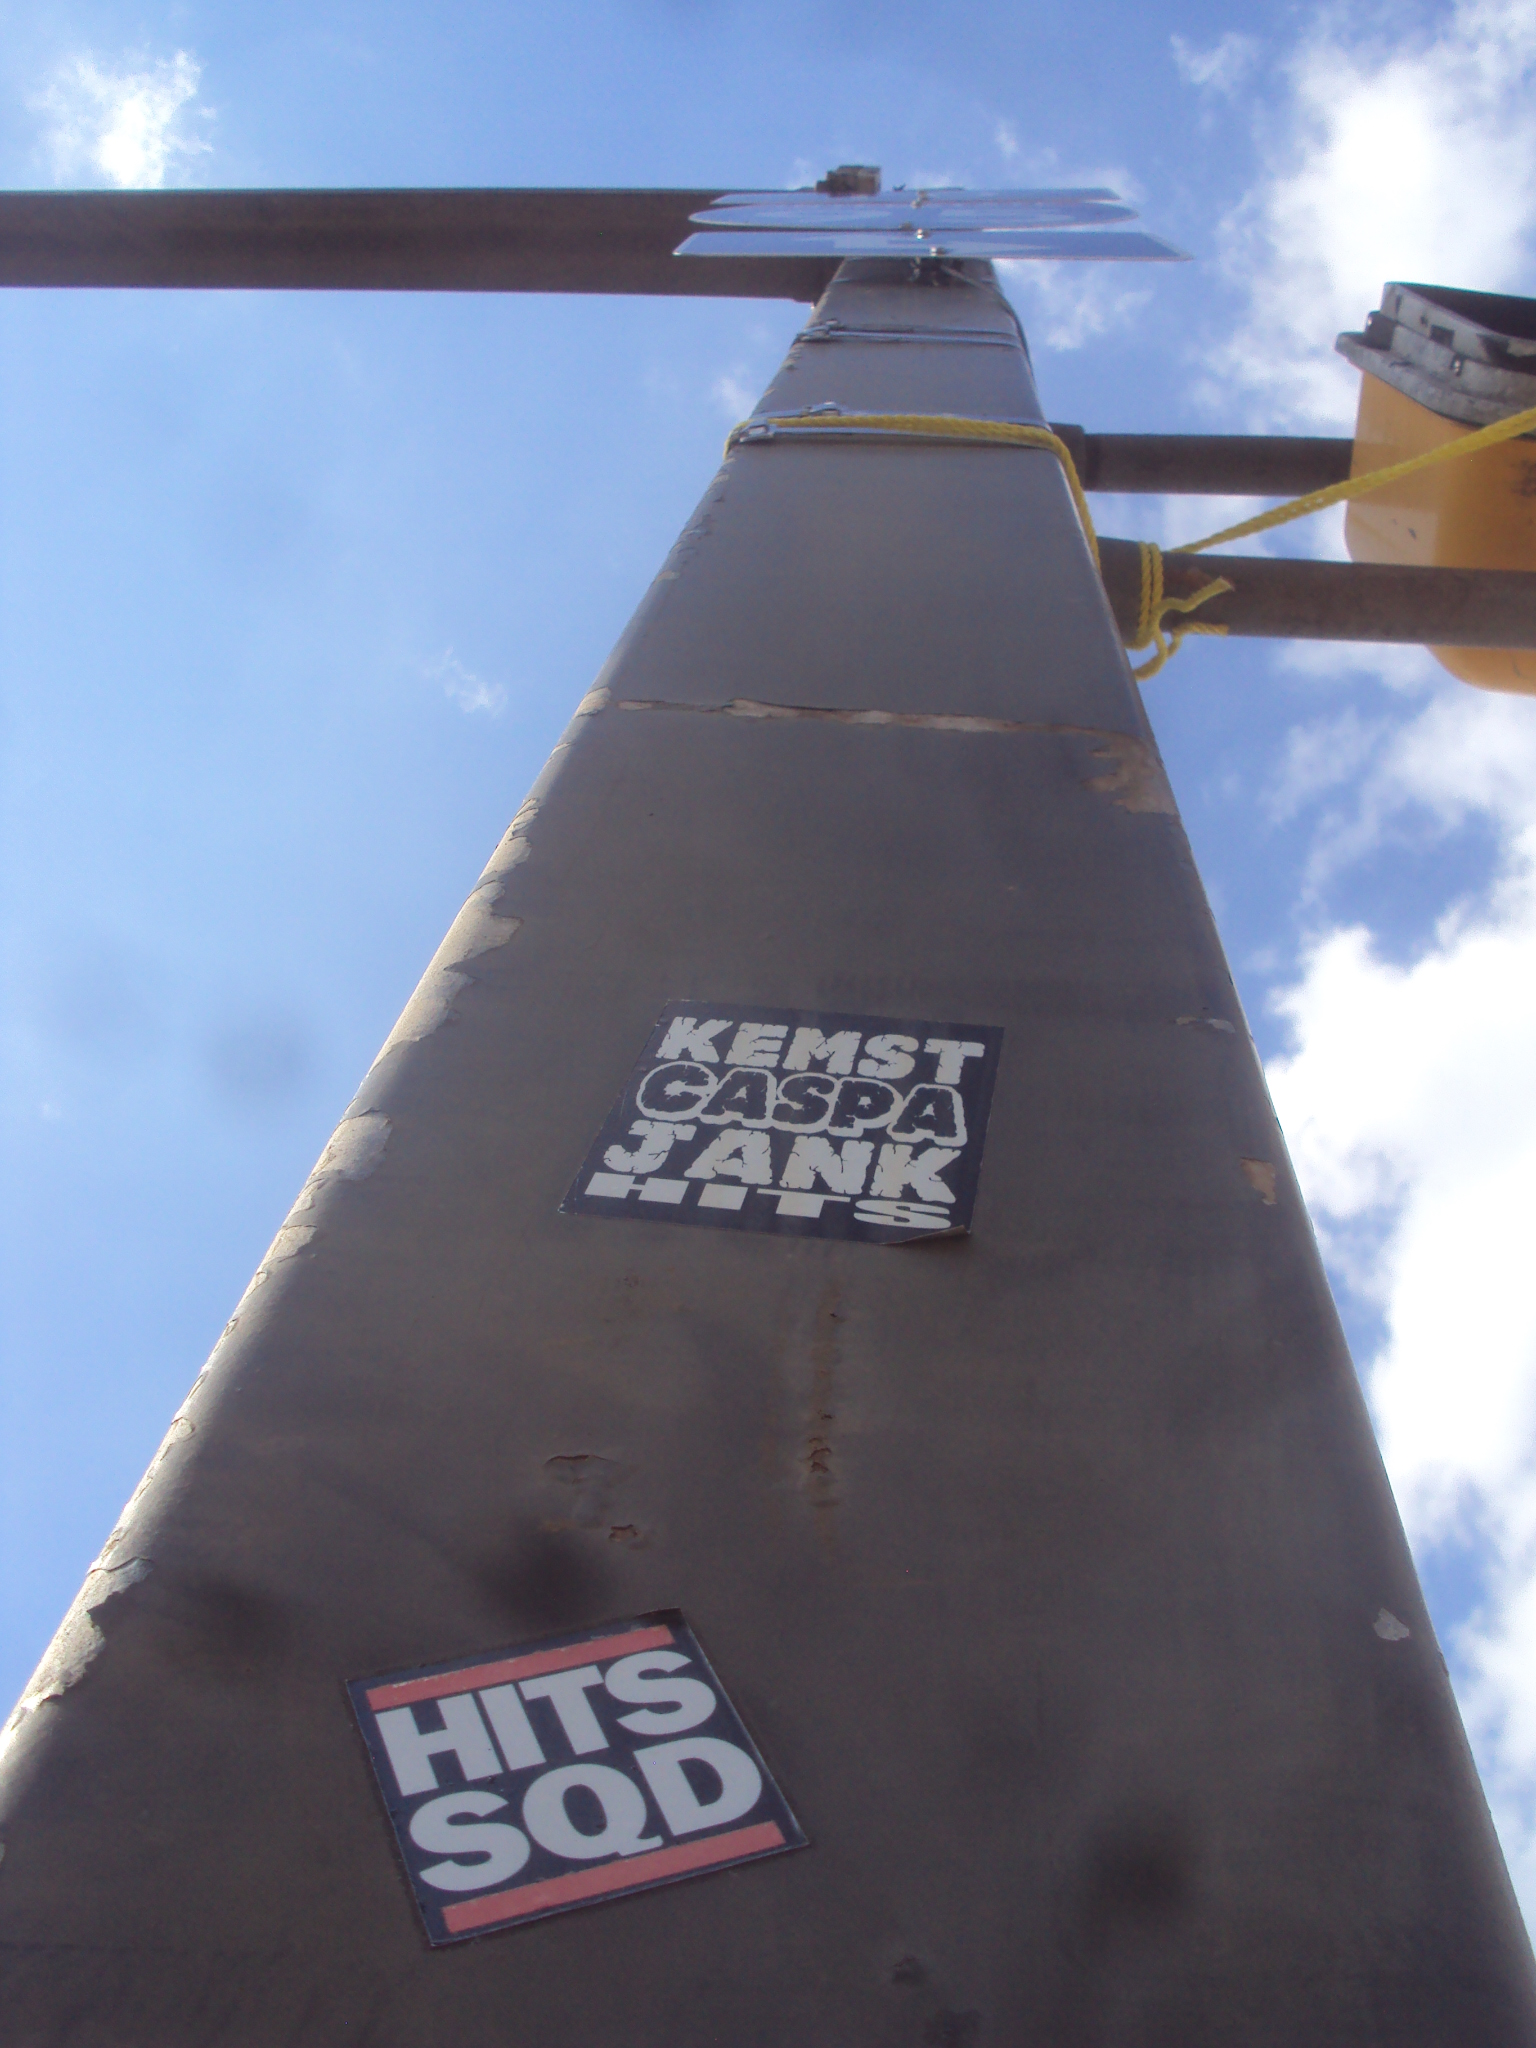
\includegraphics[height=4in]{portrait.jpg}

CAPTION L1\\
CAPTION P1\\
CAPTION P2\\
\pagebreak

% Layout PL
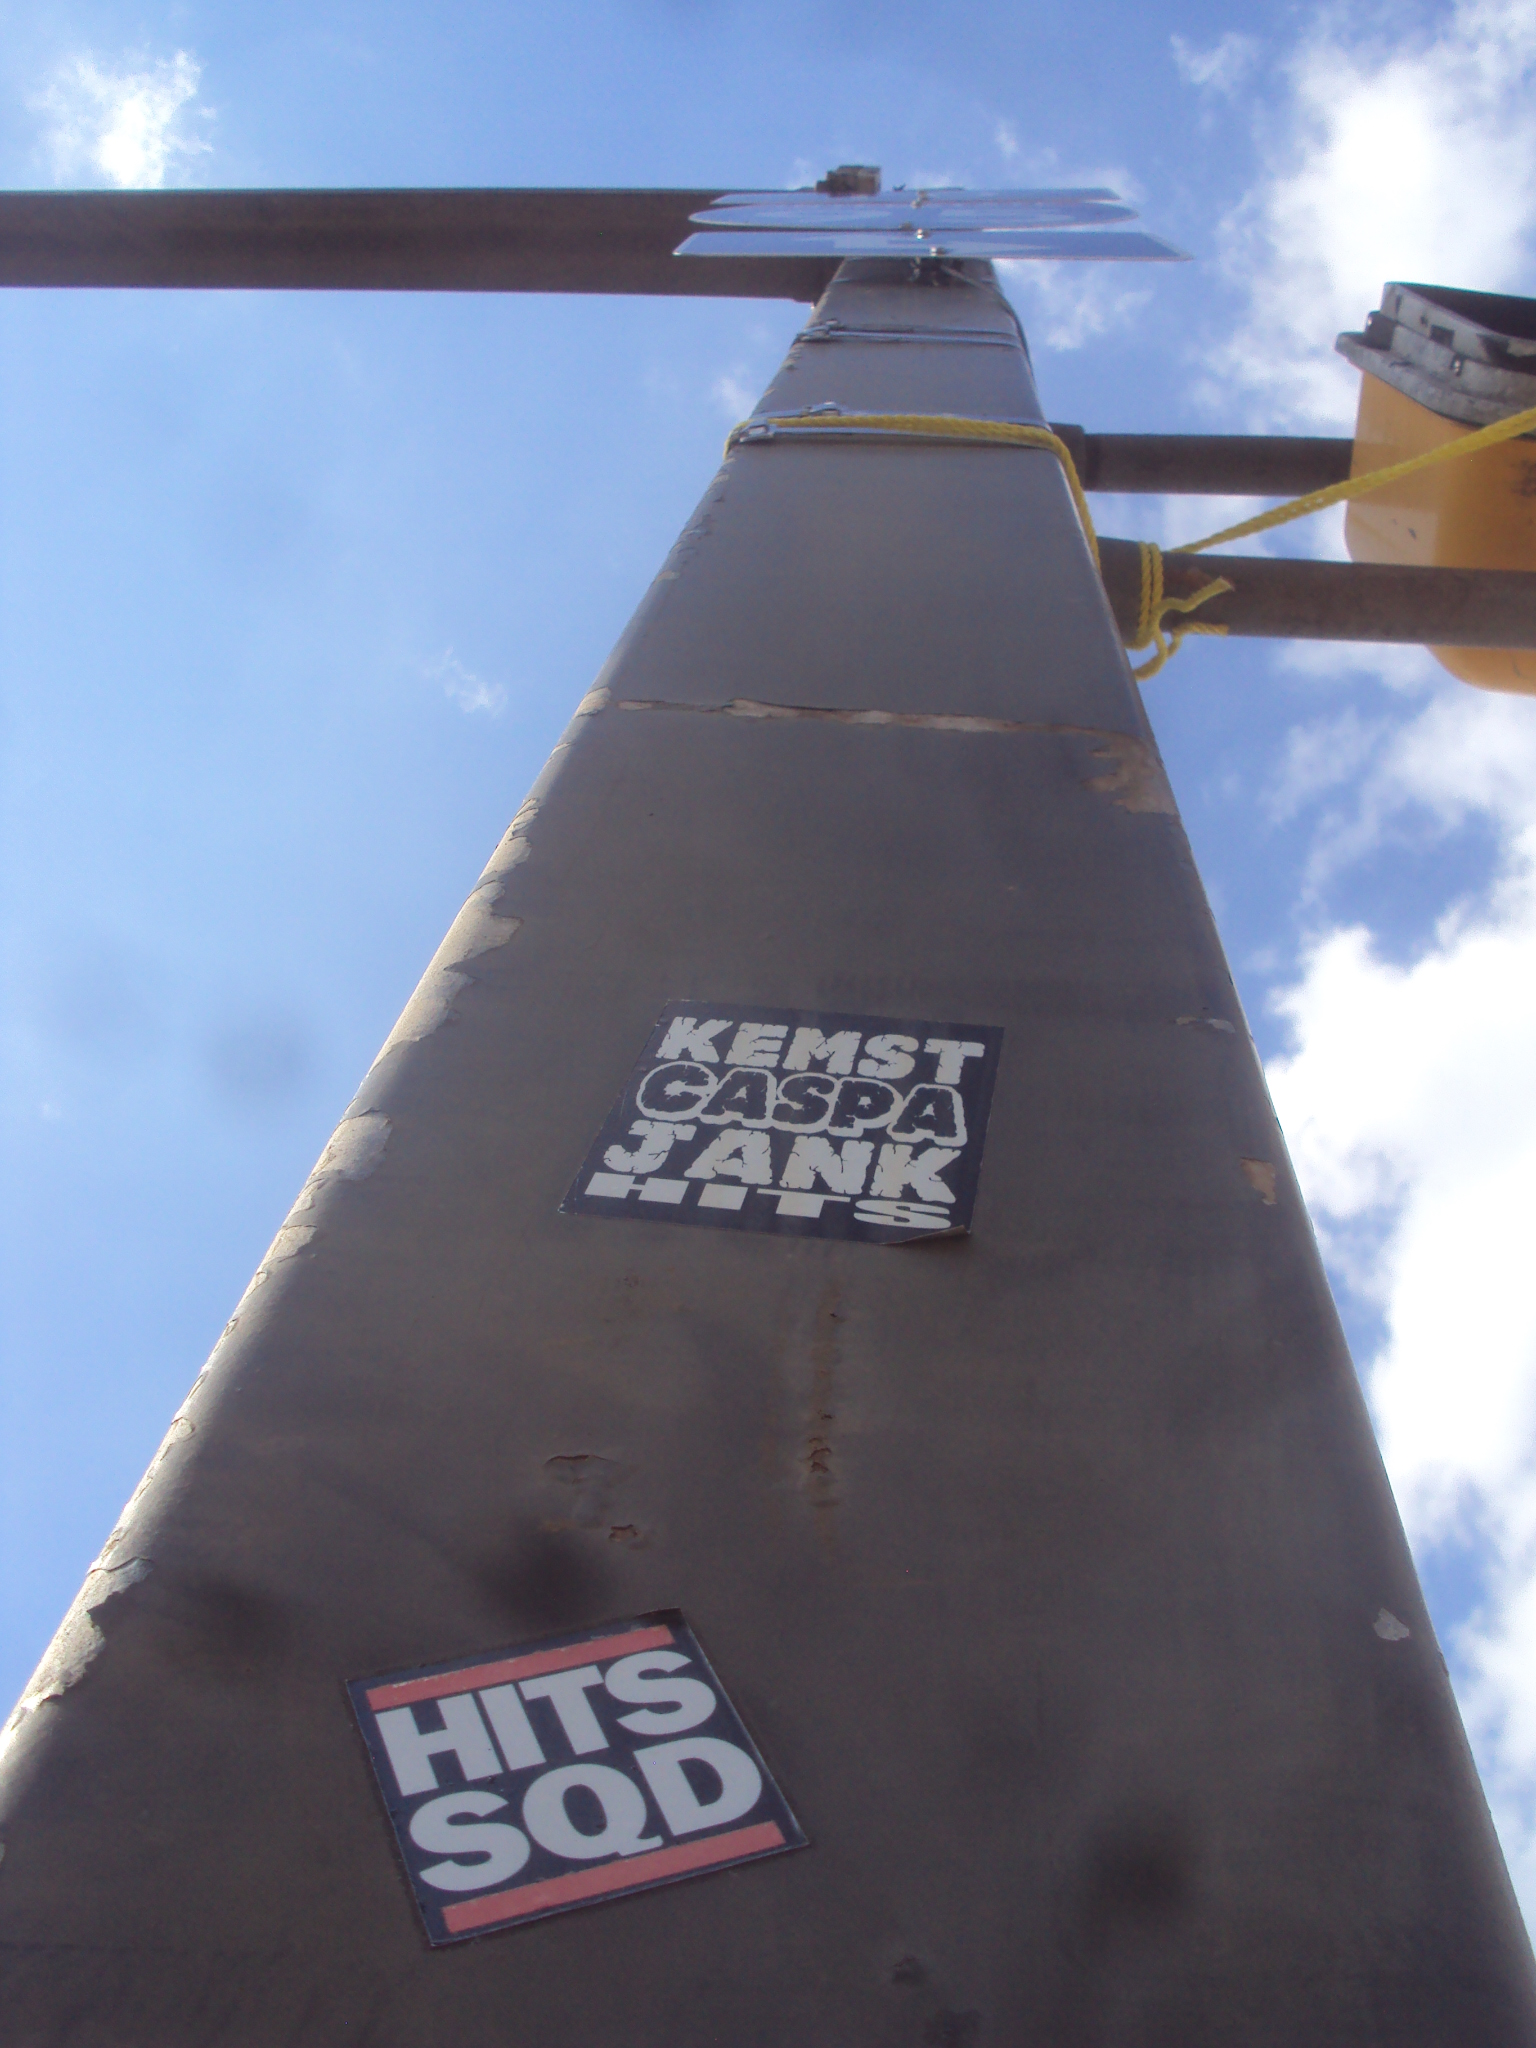
\includegraphics[height=4in]{portrait.jpg}

\vspace{0.25in}
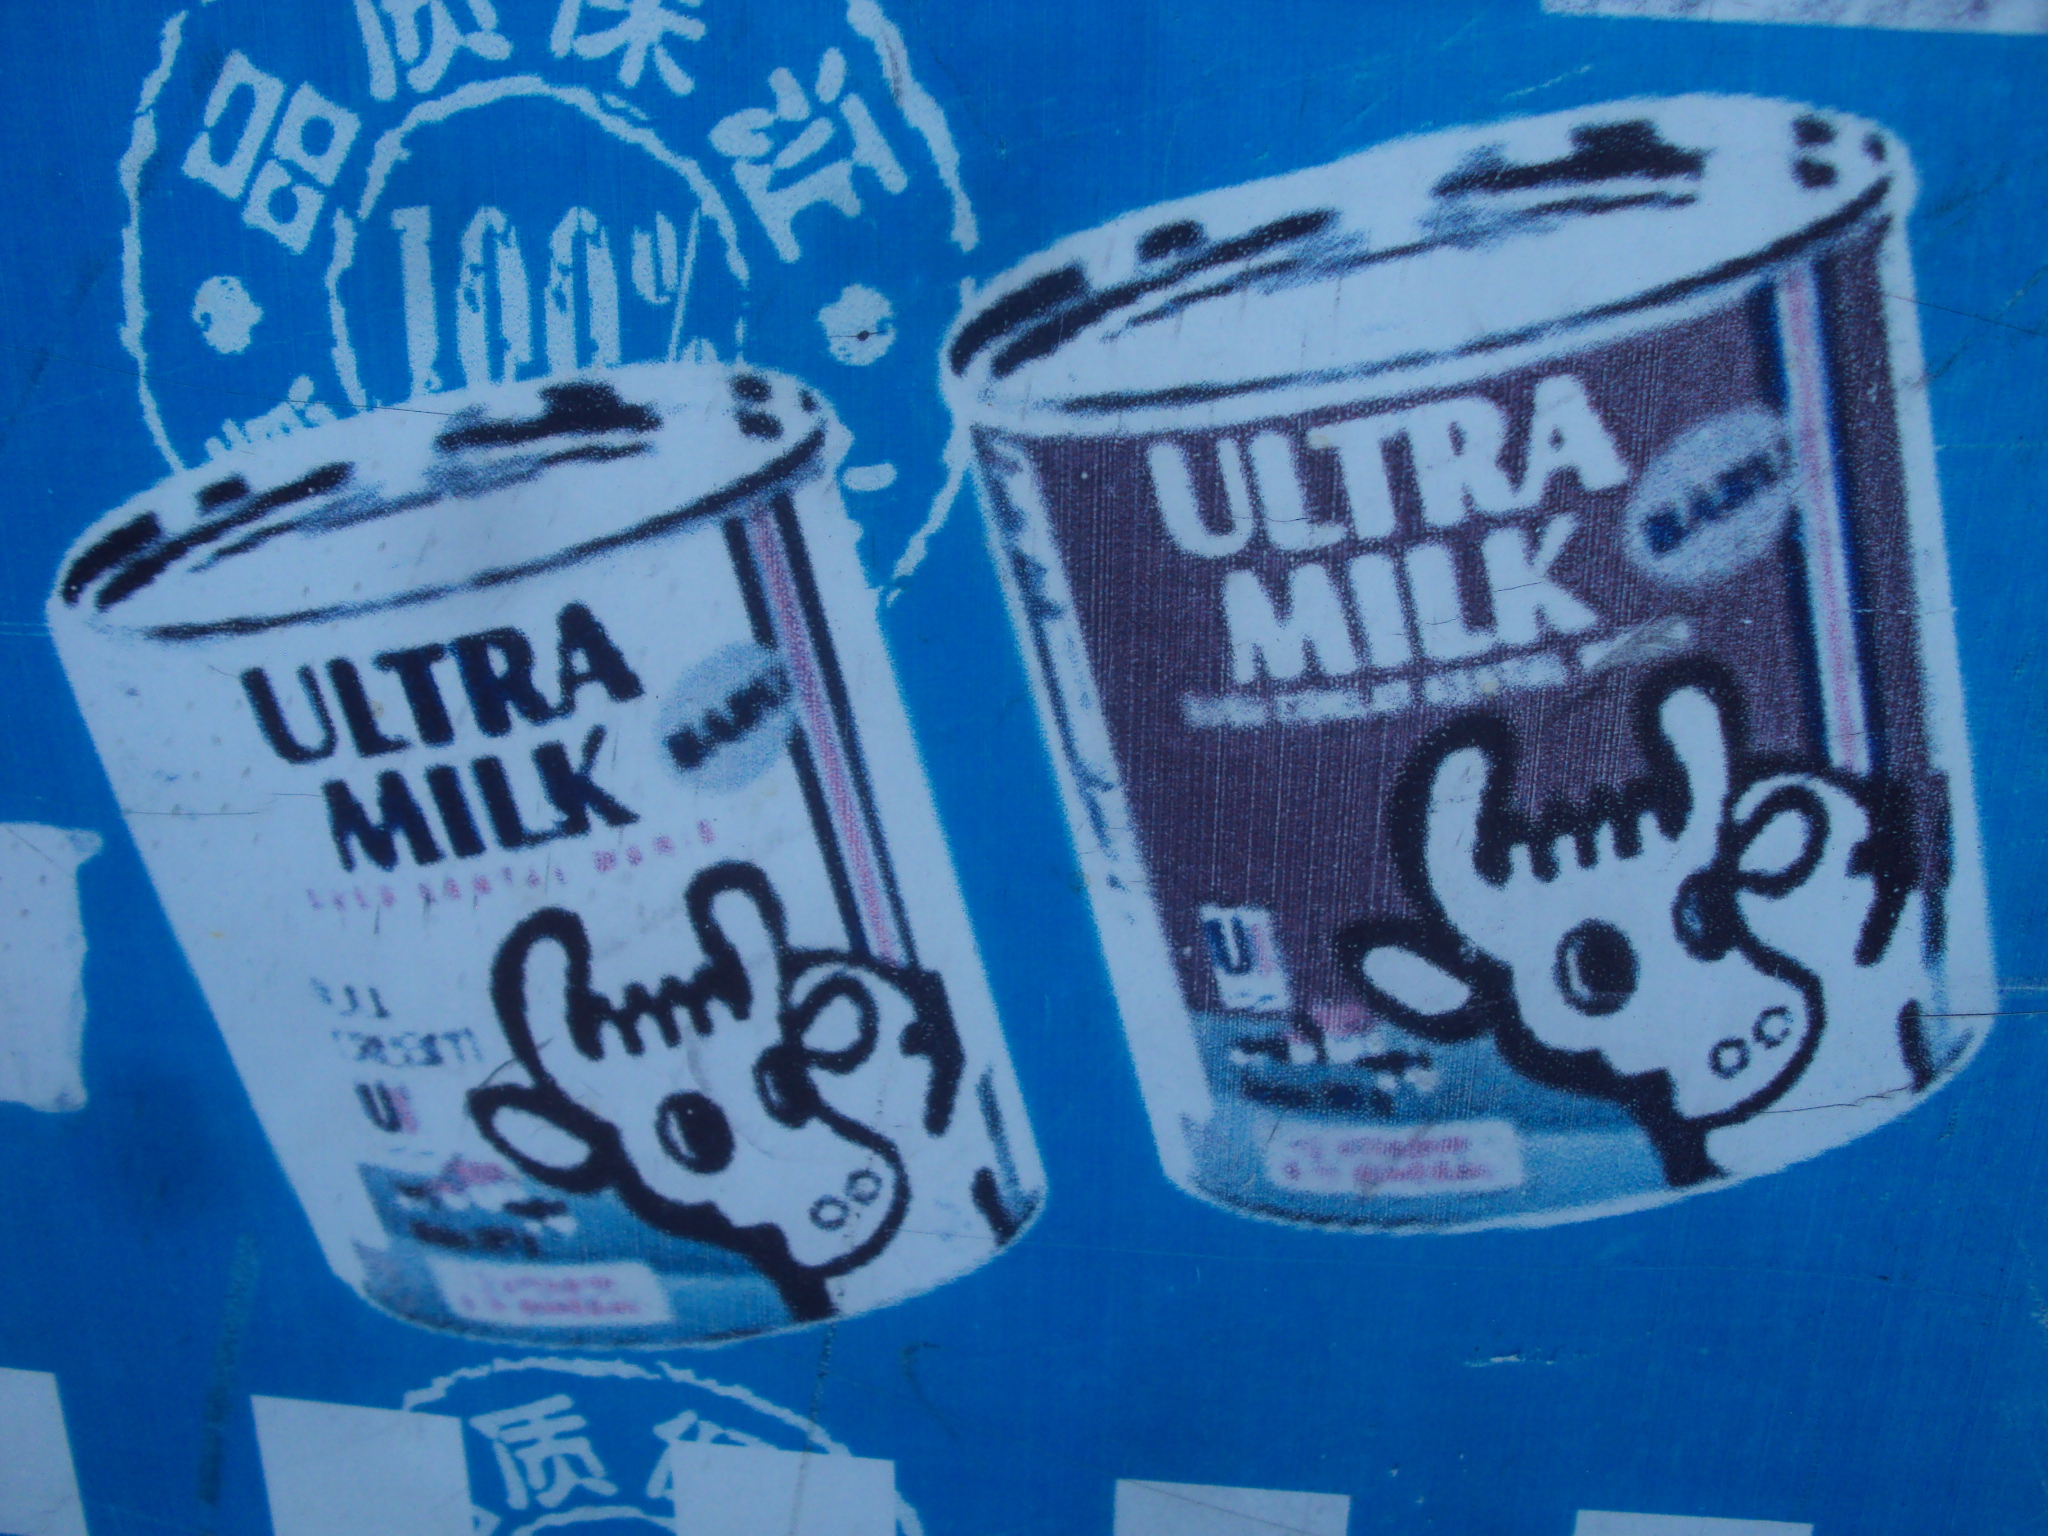
\includegraphics[width=5.19in]{landscape.jpg}

CAPTION P1\\
CAPTION L1\\
\pagebreak

% Layout LP
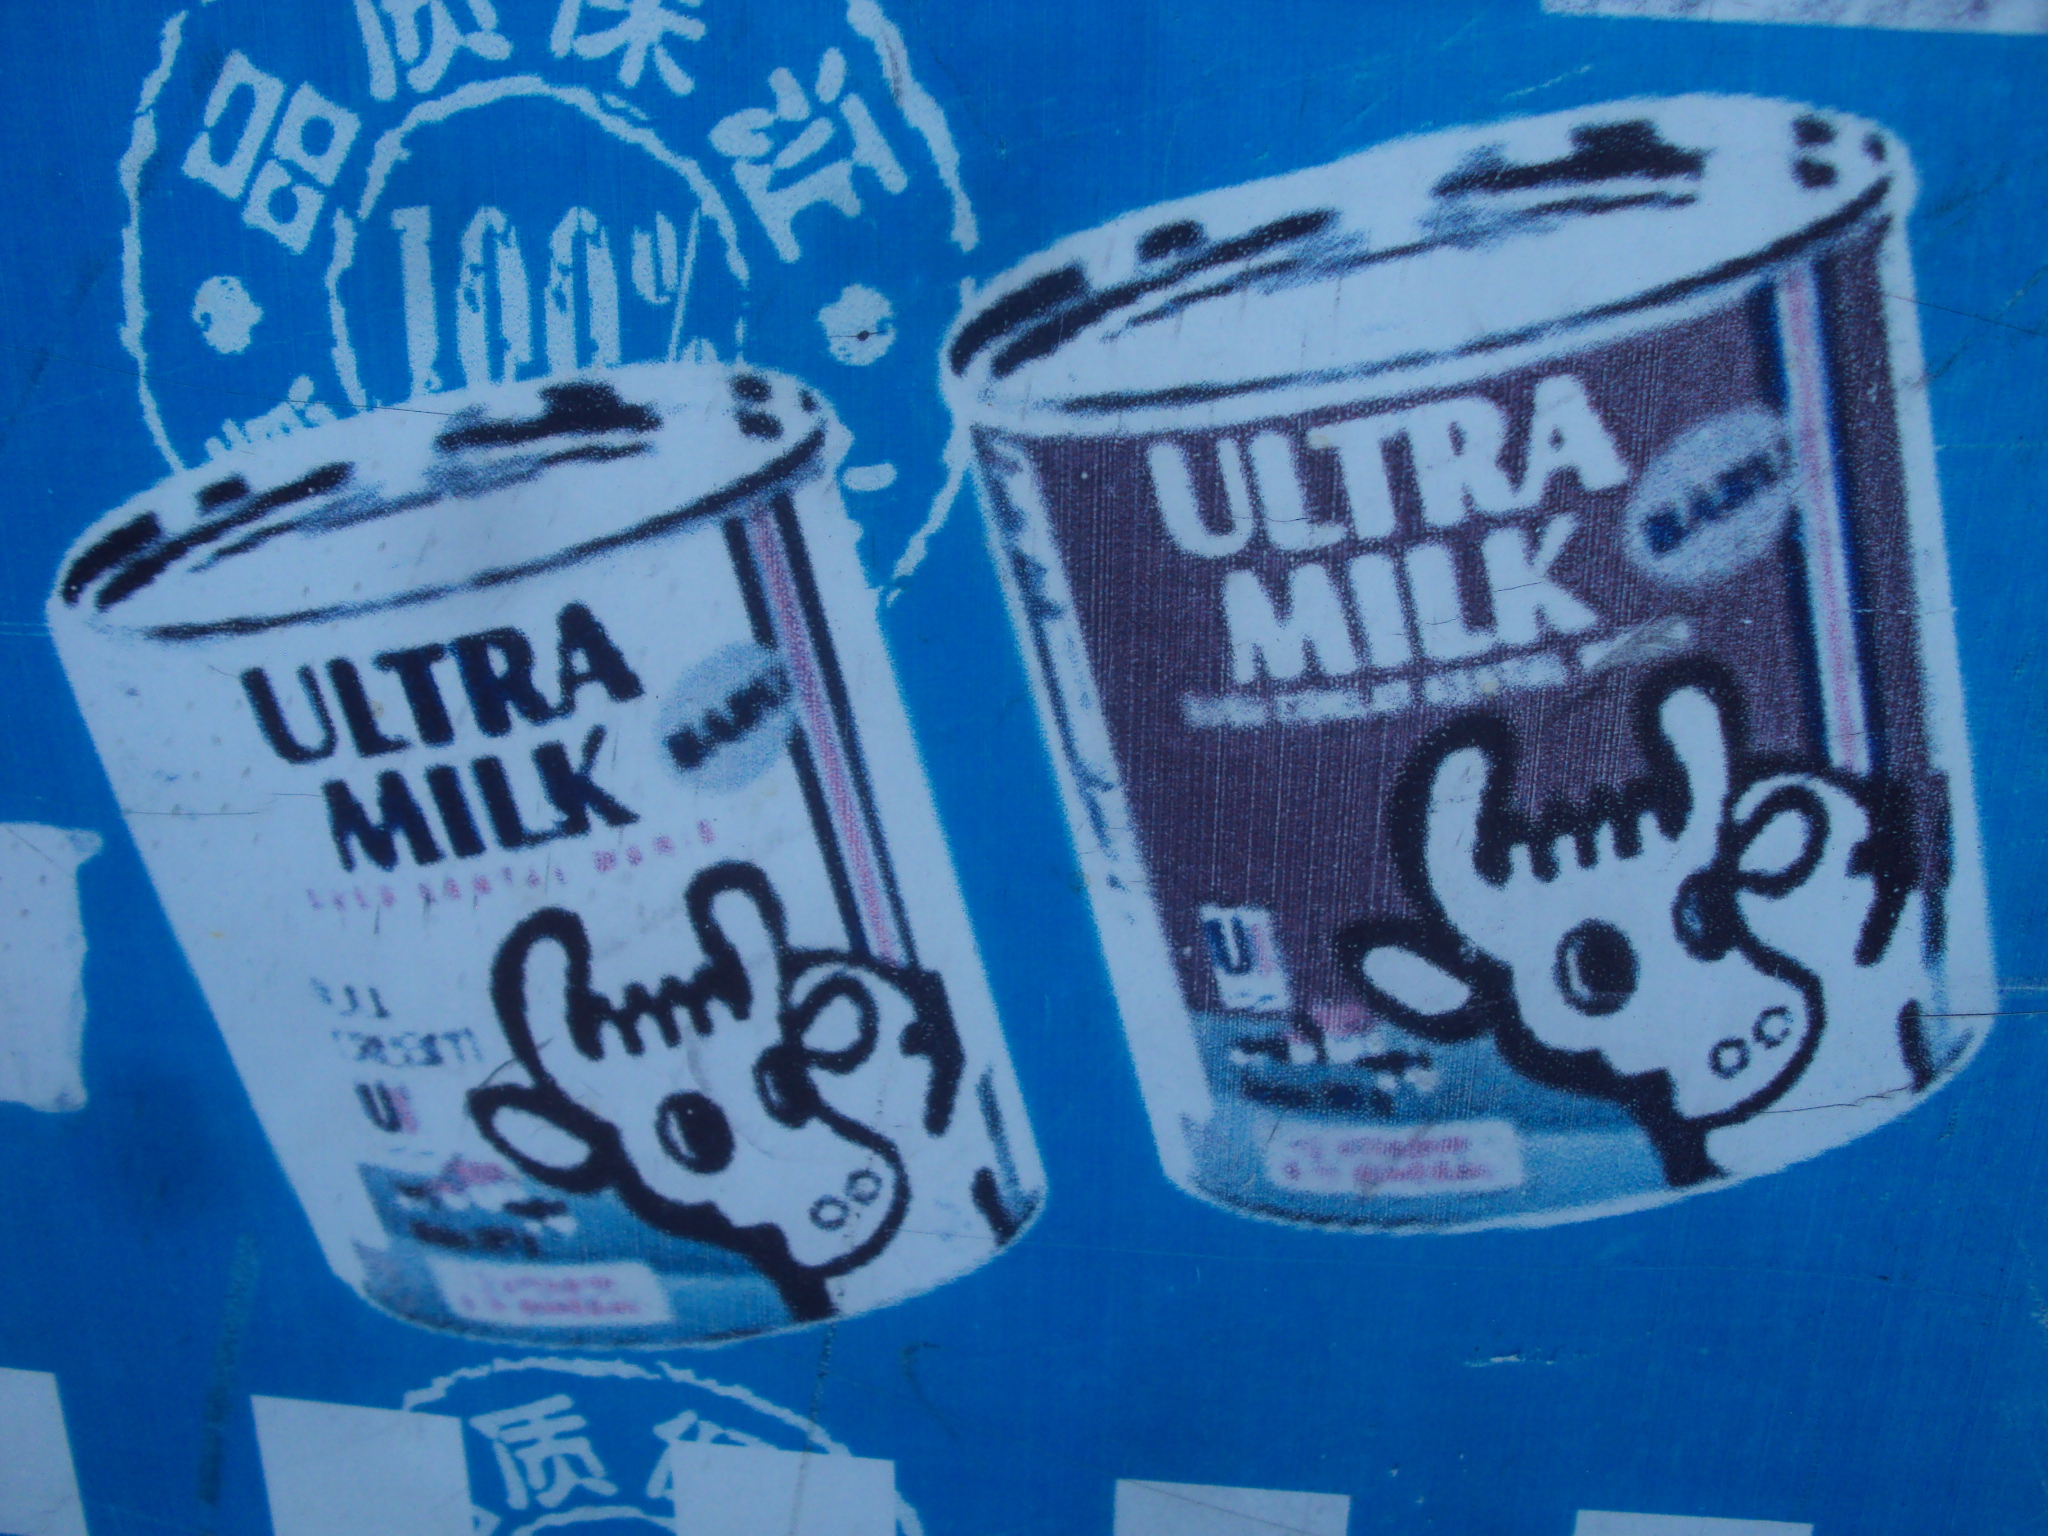
\includegraphics[width=5.19in]{landscape.jpg}

\vspace{0.25in}
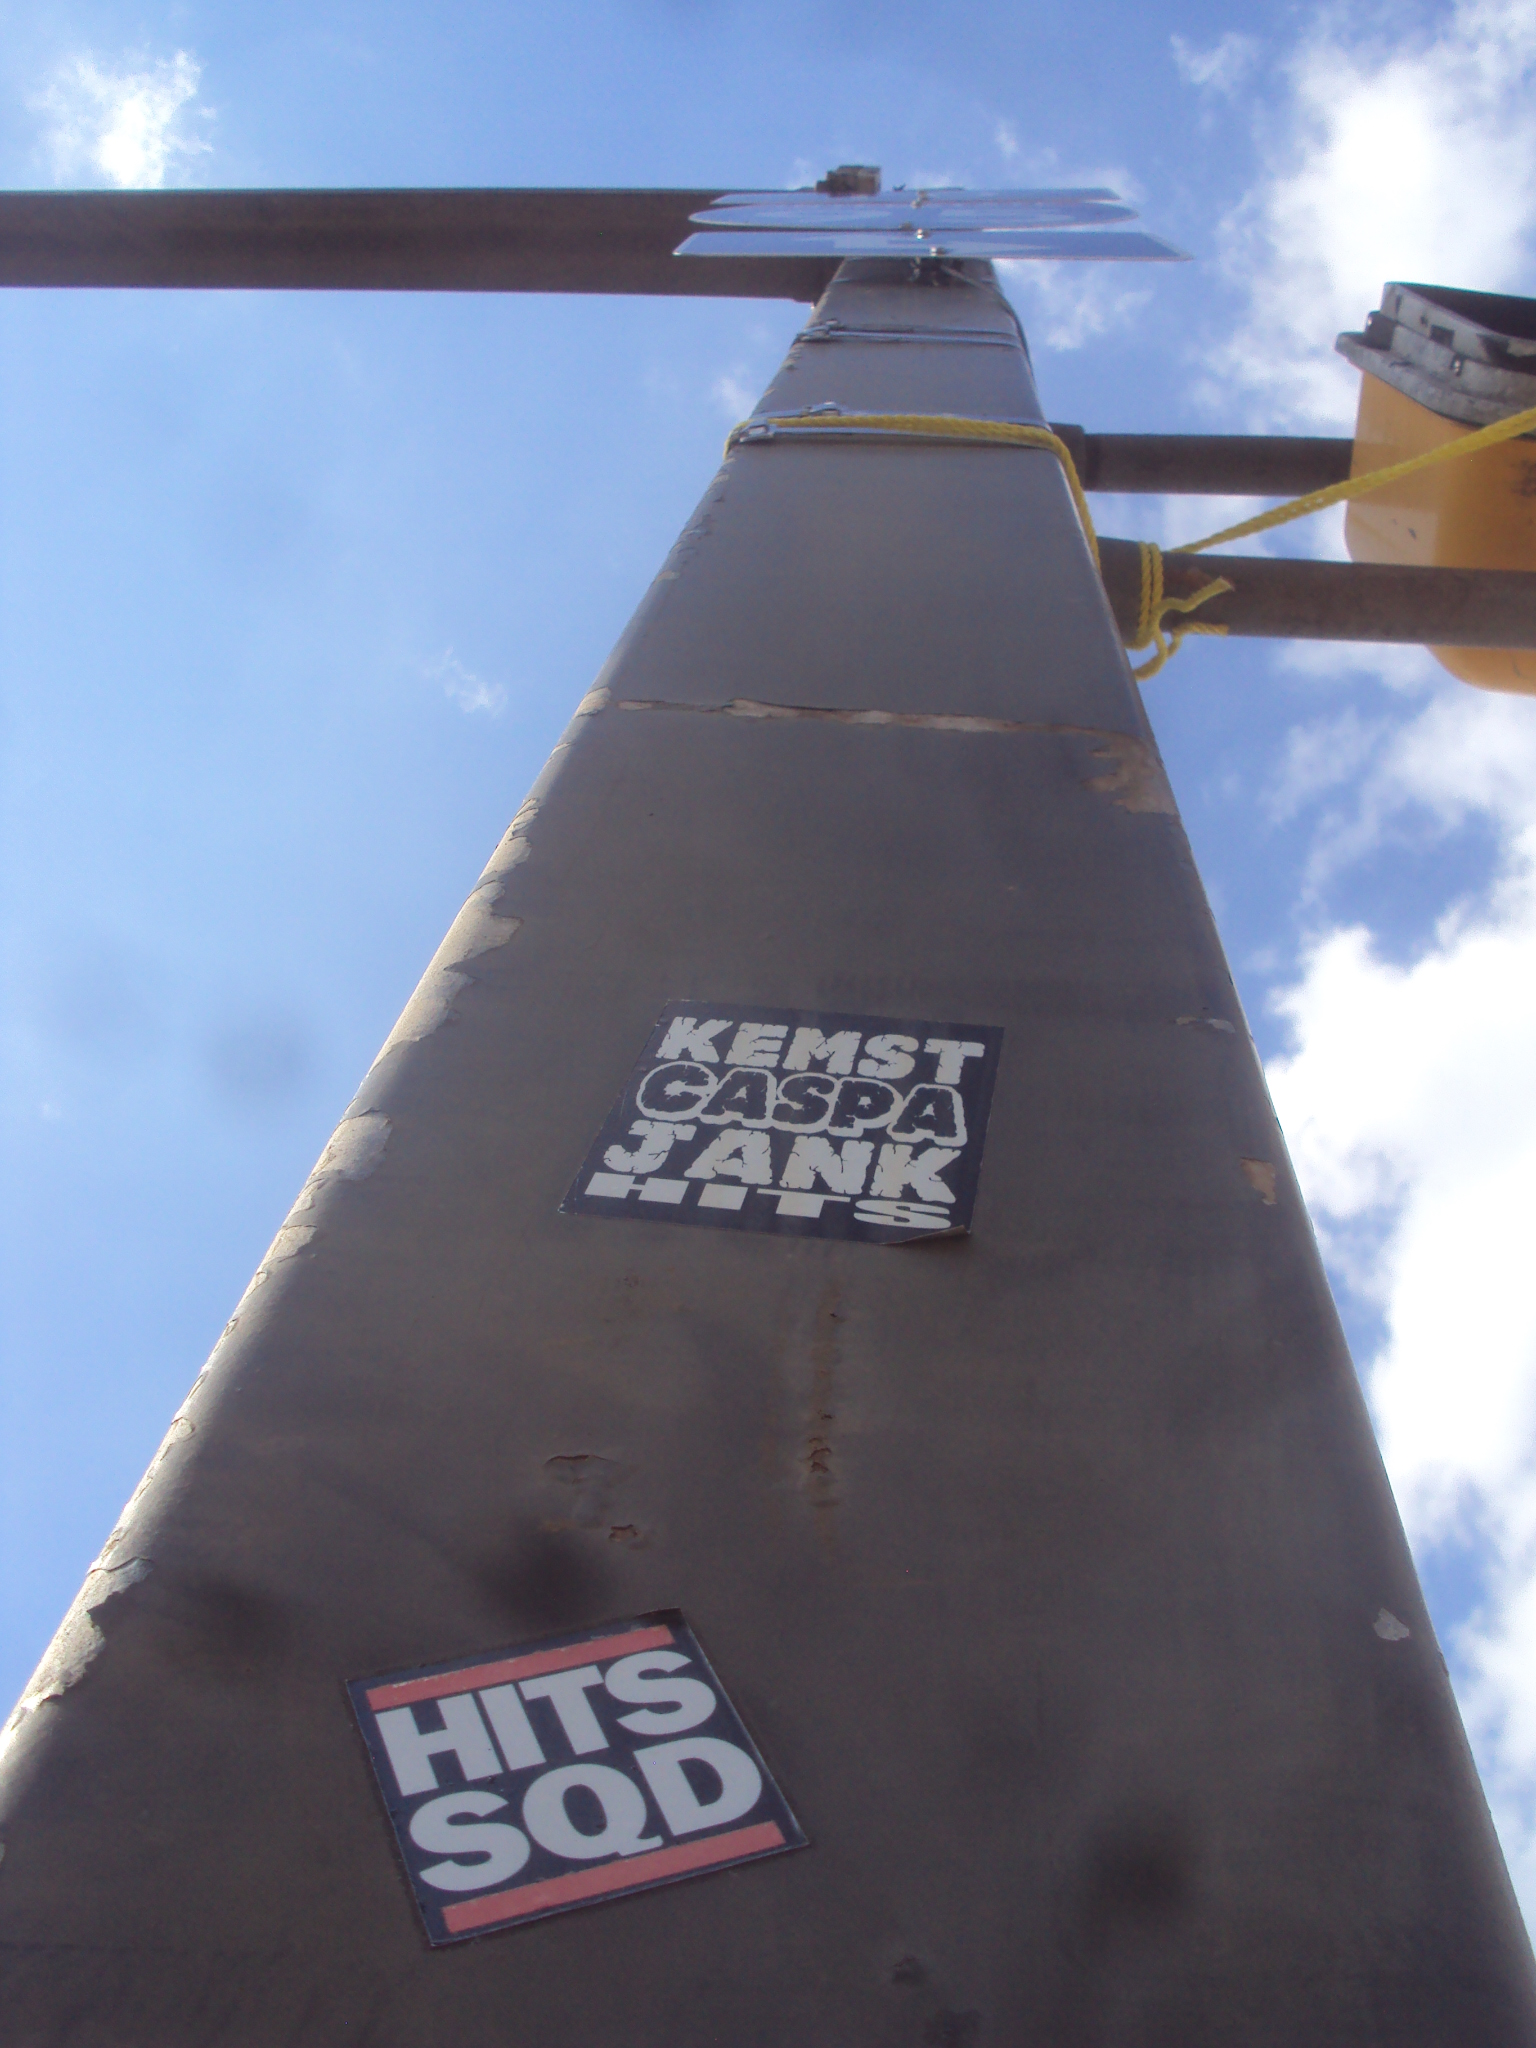
\includegraphics[height=4in]{portrait.jpg}

CAPTION L1\\
CAPTION P1\\
\pagebreak
\end{document}
